%%%%%%%%%%%%%%%%%%%%%%%%%%%%%%%%%%%%%%%%%%%%%%%%%%%%%%%%%%%%%%%%%%%%%%%%%%
%%%%%%%%%%%%%%%%%%%%%%%%%%%%%%%%%%%%%%%%%%%%%%%%%%%%%%%%%%%%%%%%%%%%%%%%%%
%%\clearpage{}
\subsection{Comparison of Data and Monte Carlo simulation}
To assess the quality of the modeling provided by the MC simulation we 
make comparisons between the MC shape normalized to the total
prediction for the background compared to the overall data
yield after applying the event selection criteria (except for b-tag requirement). 
We show the distributions of various kinematic
variables after applying all the selection cuts in 
Figures ~\ref{fig:mu_jet_pt}-\ref{fig:mu_dijet}
for the muon+jets sample and in 
Figures ~\ref{fig:elec_jet_pt}-\ref{fig:elec_dijet} for
the electron+jets sample. 
Overall, there is reasonable agreement between data and simulation 
after analysis-level selection.
Although there are some notable differences in few places 
(\textit{e. g.}, in the jet $p_T$ spectra of Fig.~\ref{fig:mu_jet_pt} 
and Fig.~\ref{fig:elec_jet_pt} at high $p_T$ values),  
a part of the difference in each case 
is likely caused by the small size ($\approx 0.5 \times$ data)
of W+jets simulation sample. 
Seeing reasonable agreement gives us confidence in
the qualitative aspects of the MC modeling. 

%%%%%%%%%%%%%%%%%%%%%%%%%%%%
\begin{figure}[h!t]
  {\centering
    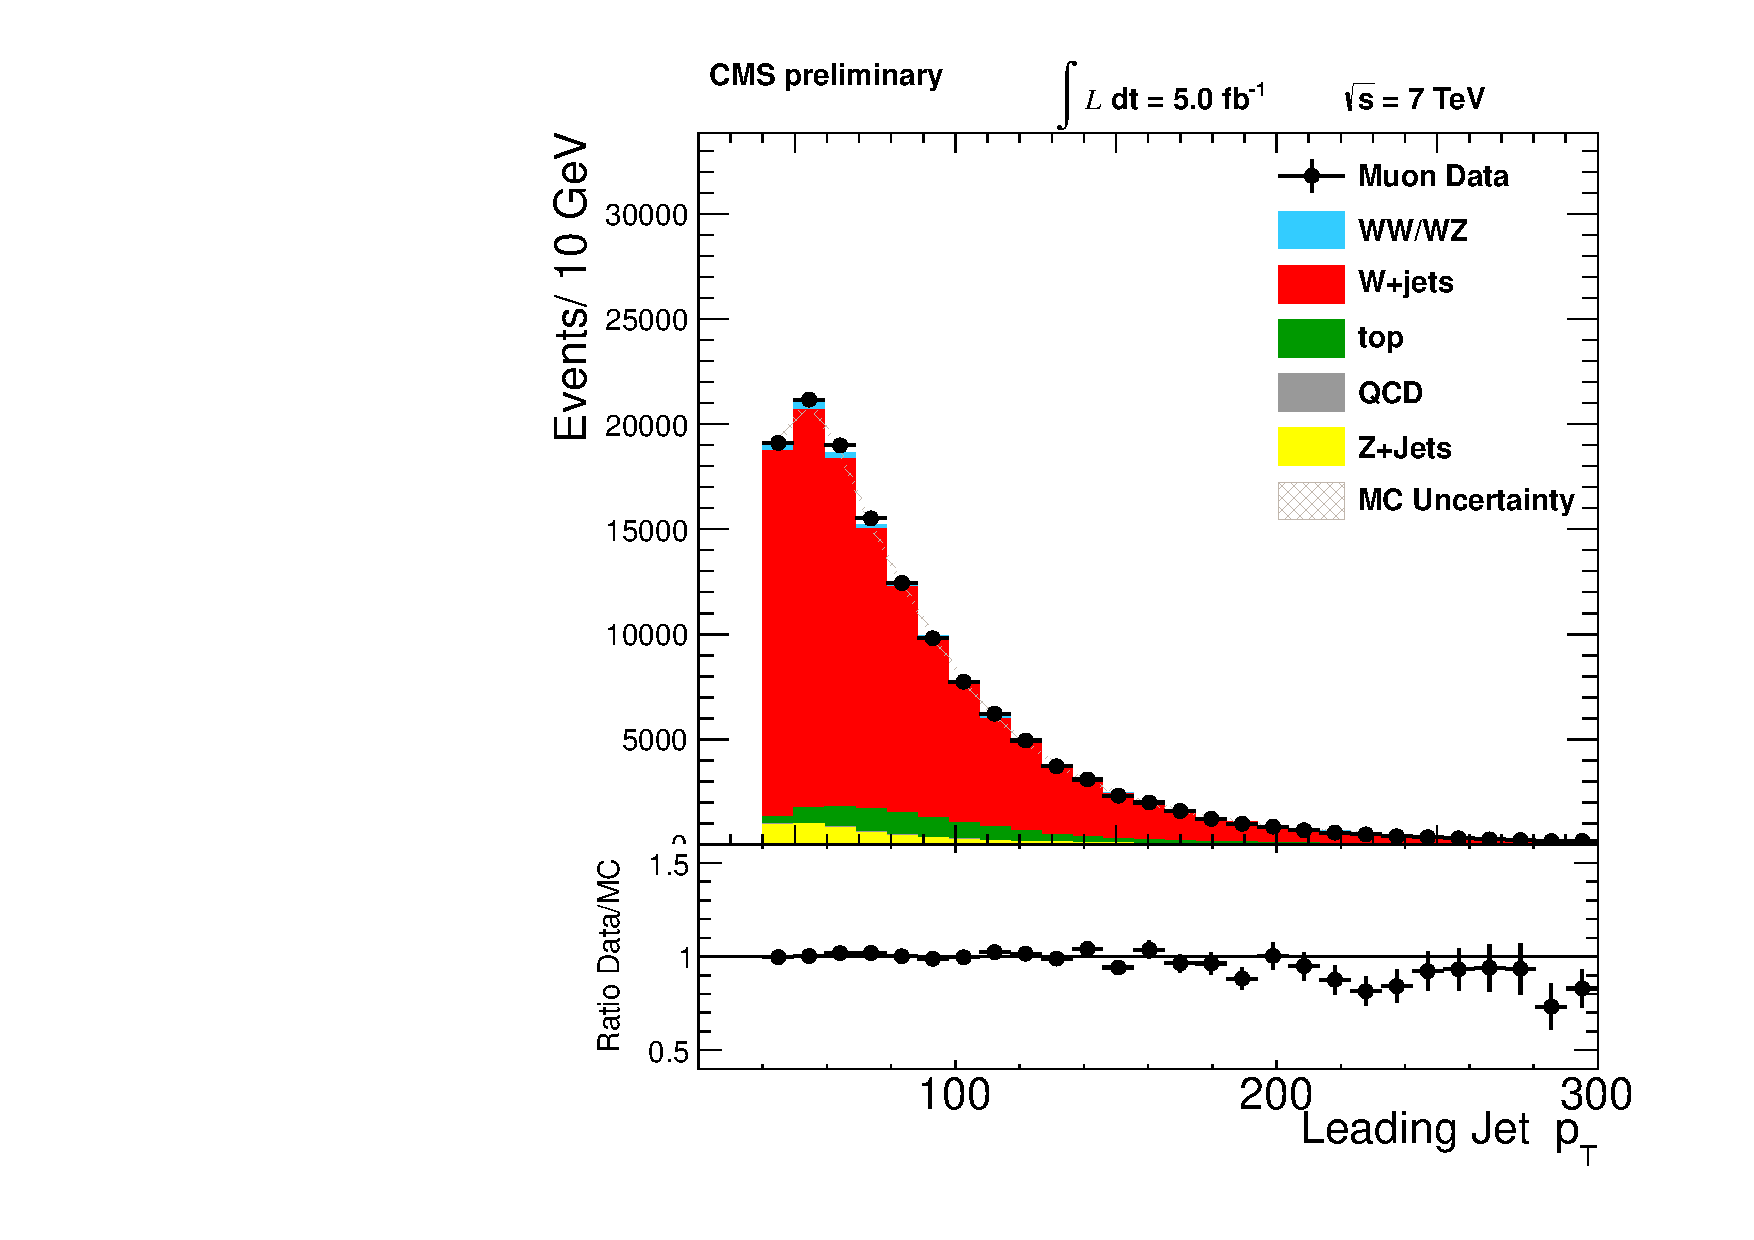
\includegraphics[width=0.49\textwidth]{figs/n-1_plots_mu/mu_jetld_pt.pdf}
    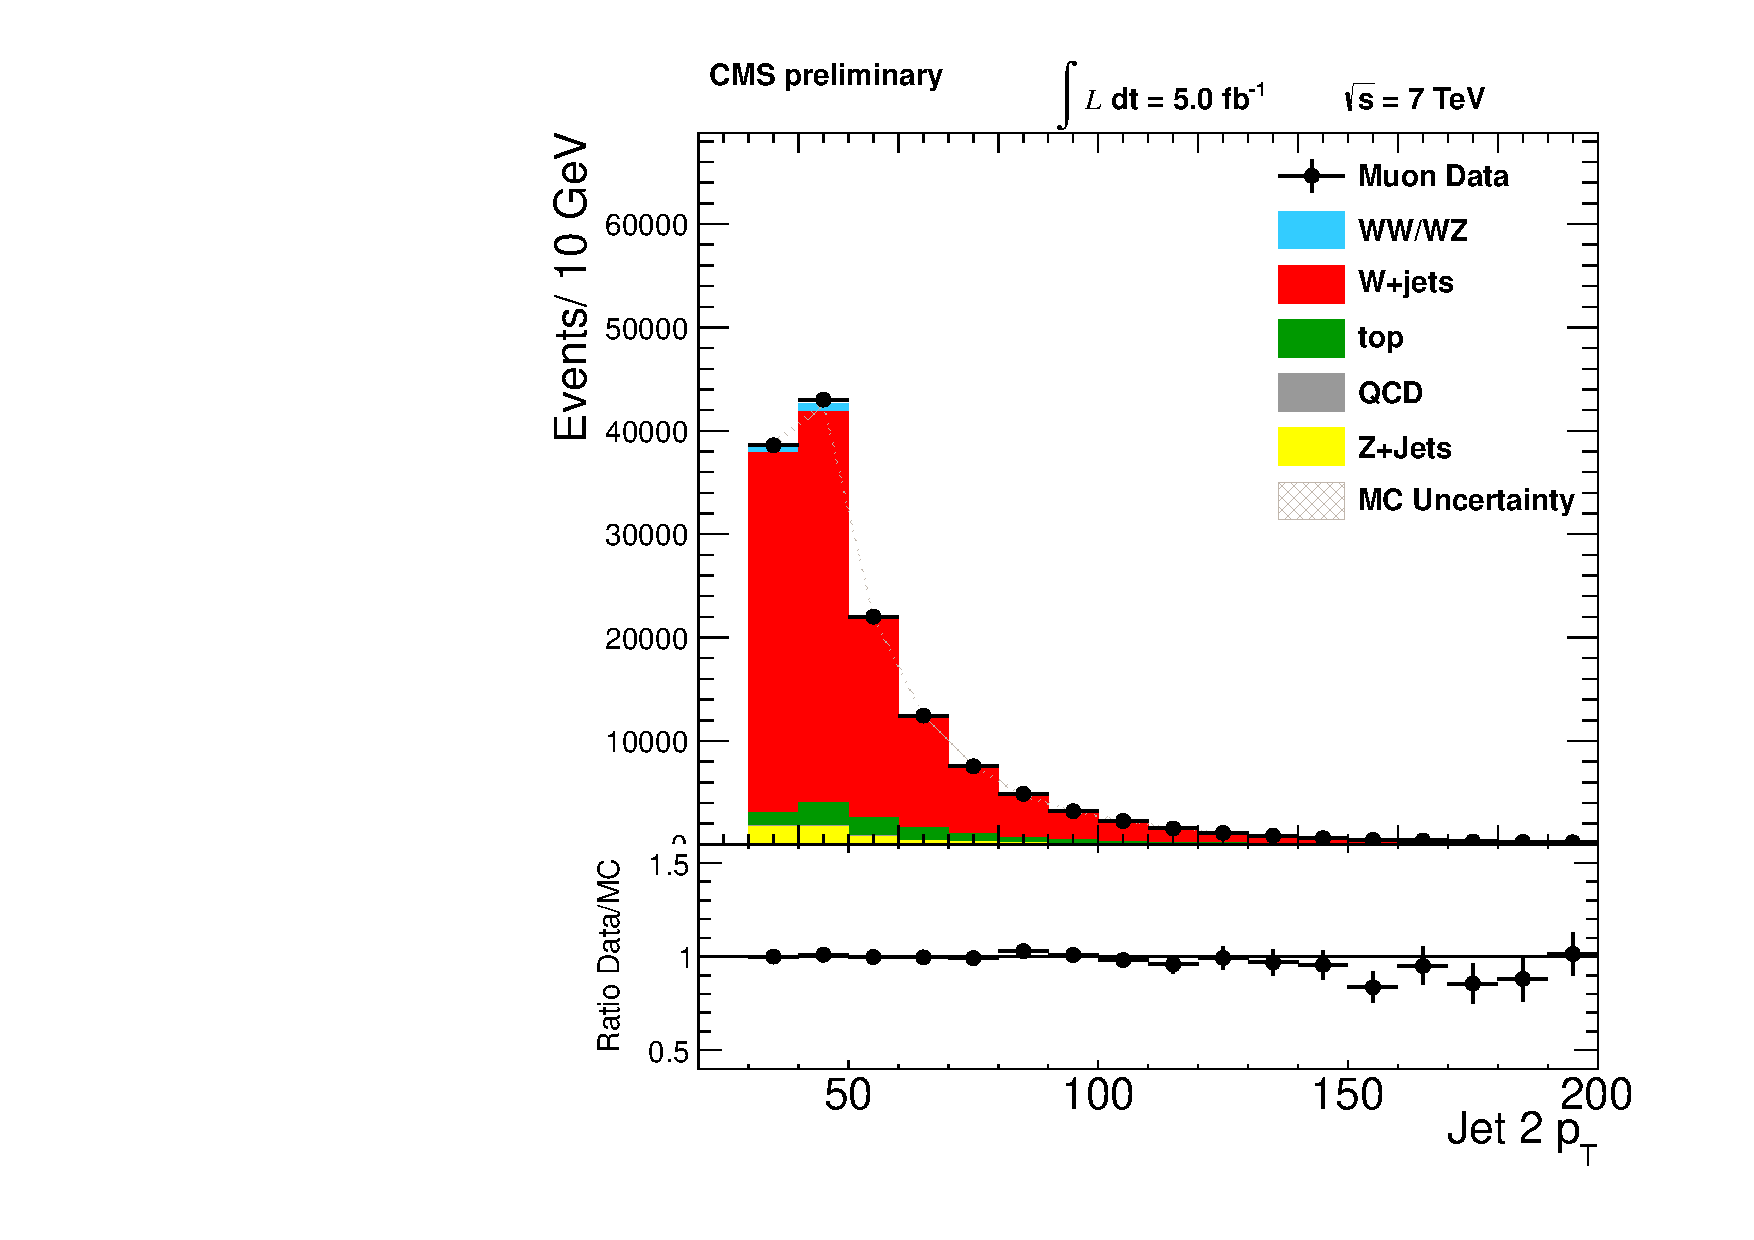
\includegraphics[width=0.49\textwidth]{figs/n-1_plots_mu/mu_jetnt_pt.pdf}
    \caption{Comparison of the leading jet (left) and 
      the second jet (right) $p_{T}$ distributions from data and MC for the muon+jets
      selection.}
    \label{fig:mu_jet_pt}}
\end{figure}
%%%%%%%%%%%%%%%%%%%%%%%%%%%%
\begin{figure}[h!t]
  {\centering
    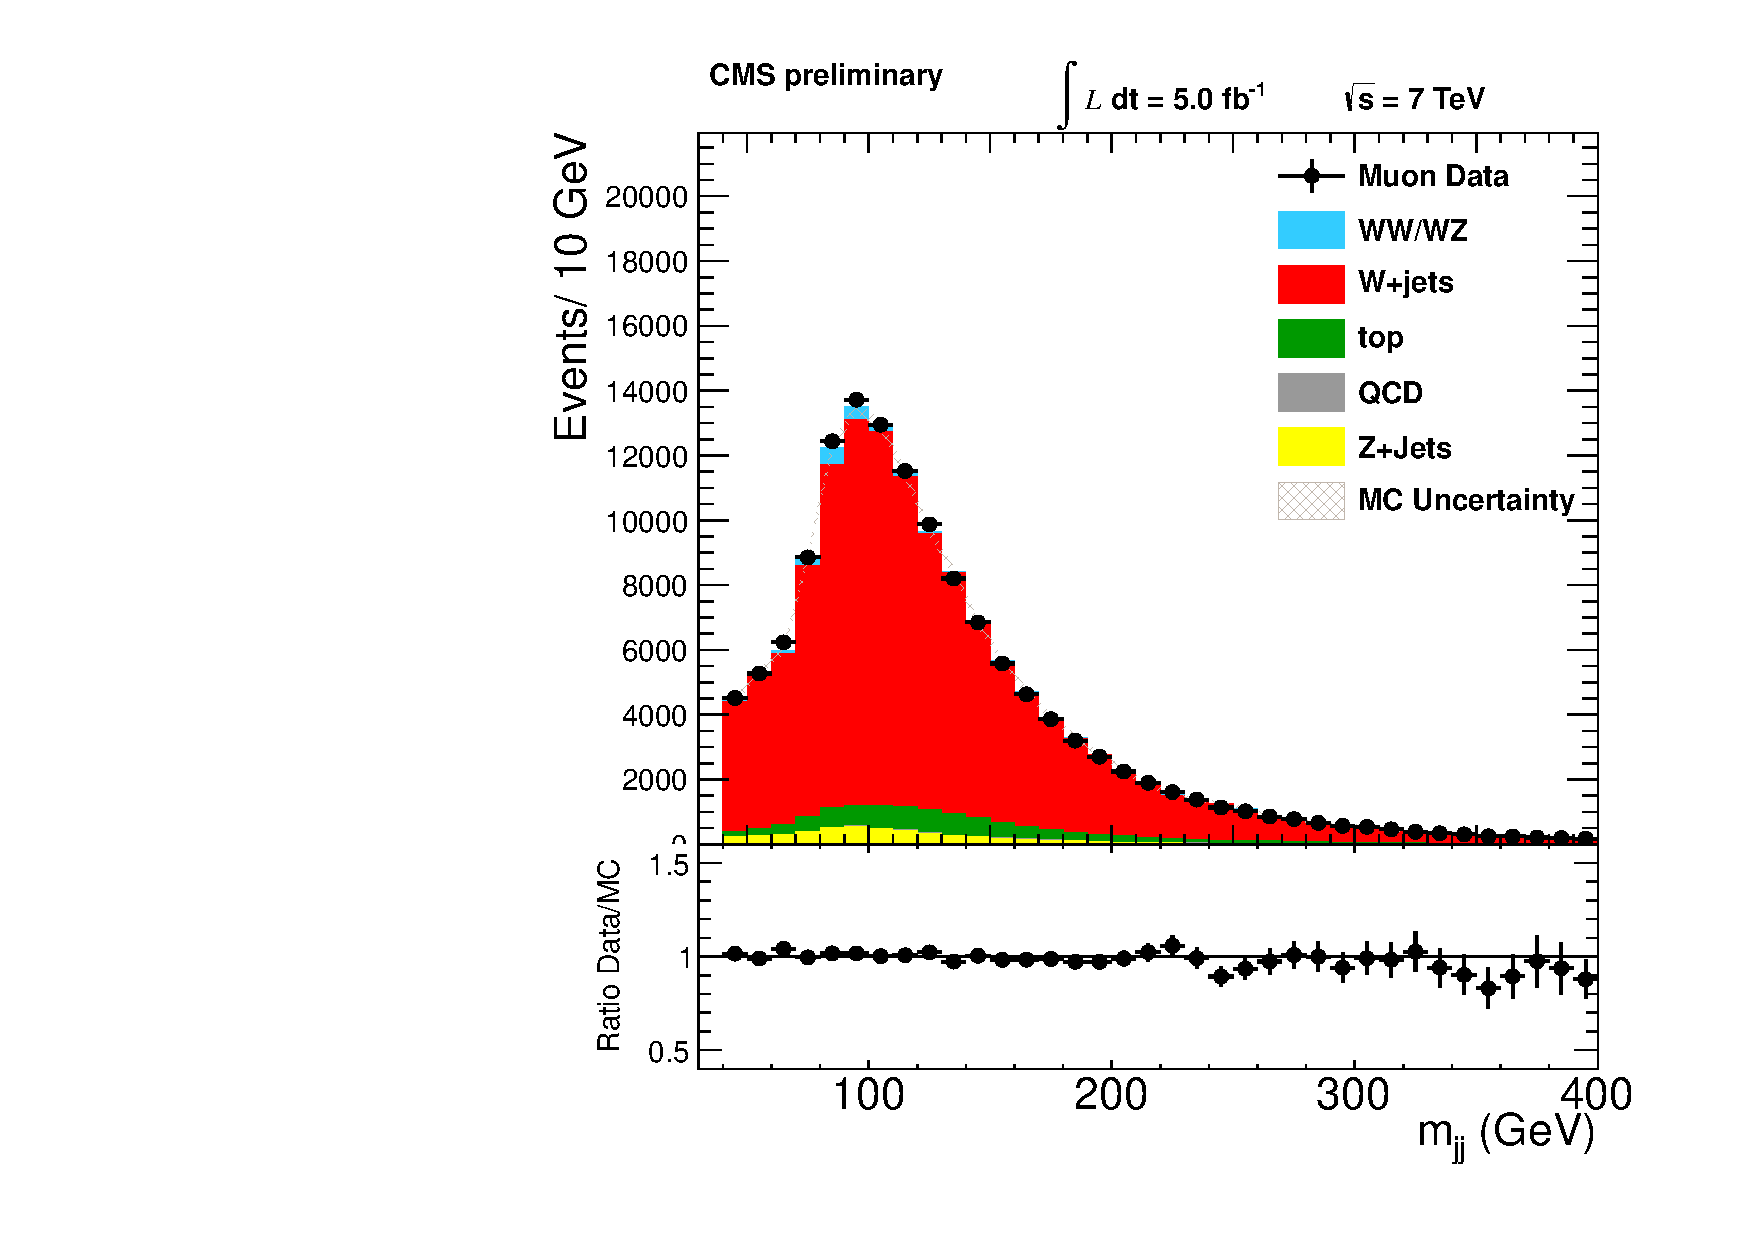
\includegraphics[width=0.49\textwidth]{figs/n-1_plots_mu/mu_mjj.pdf}
    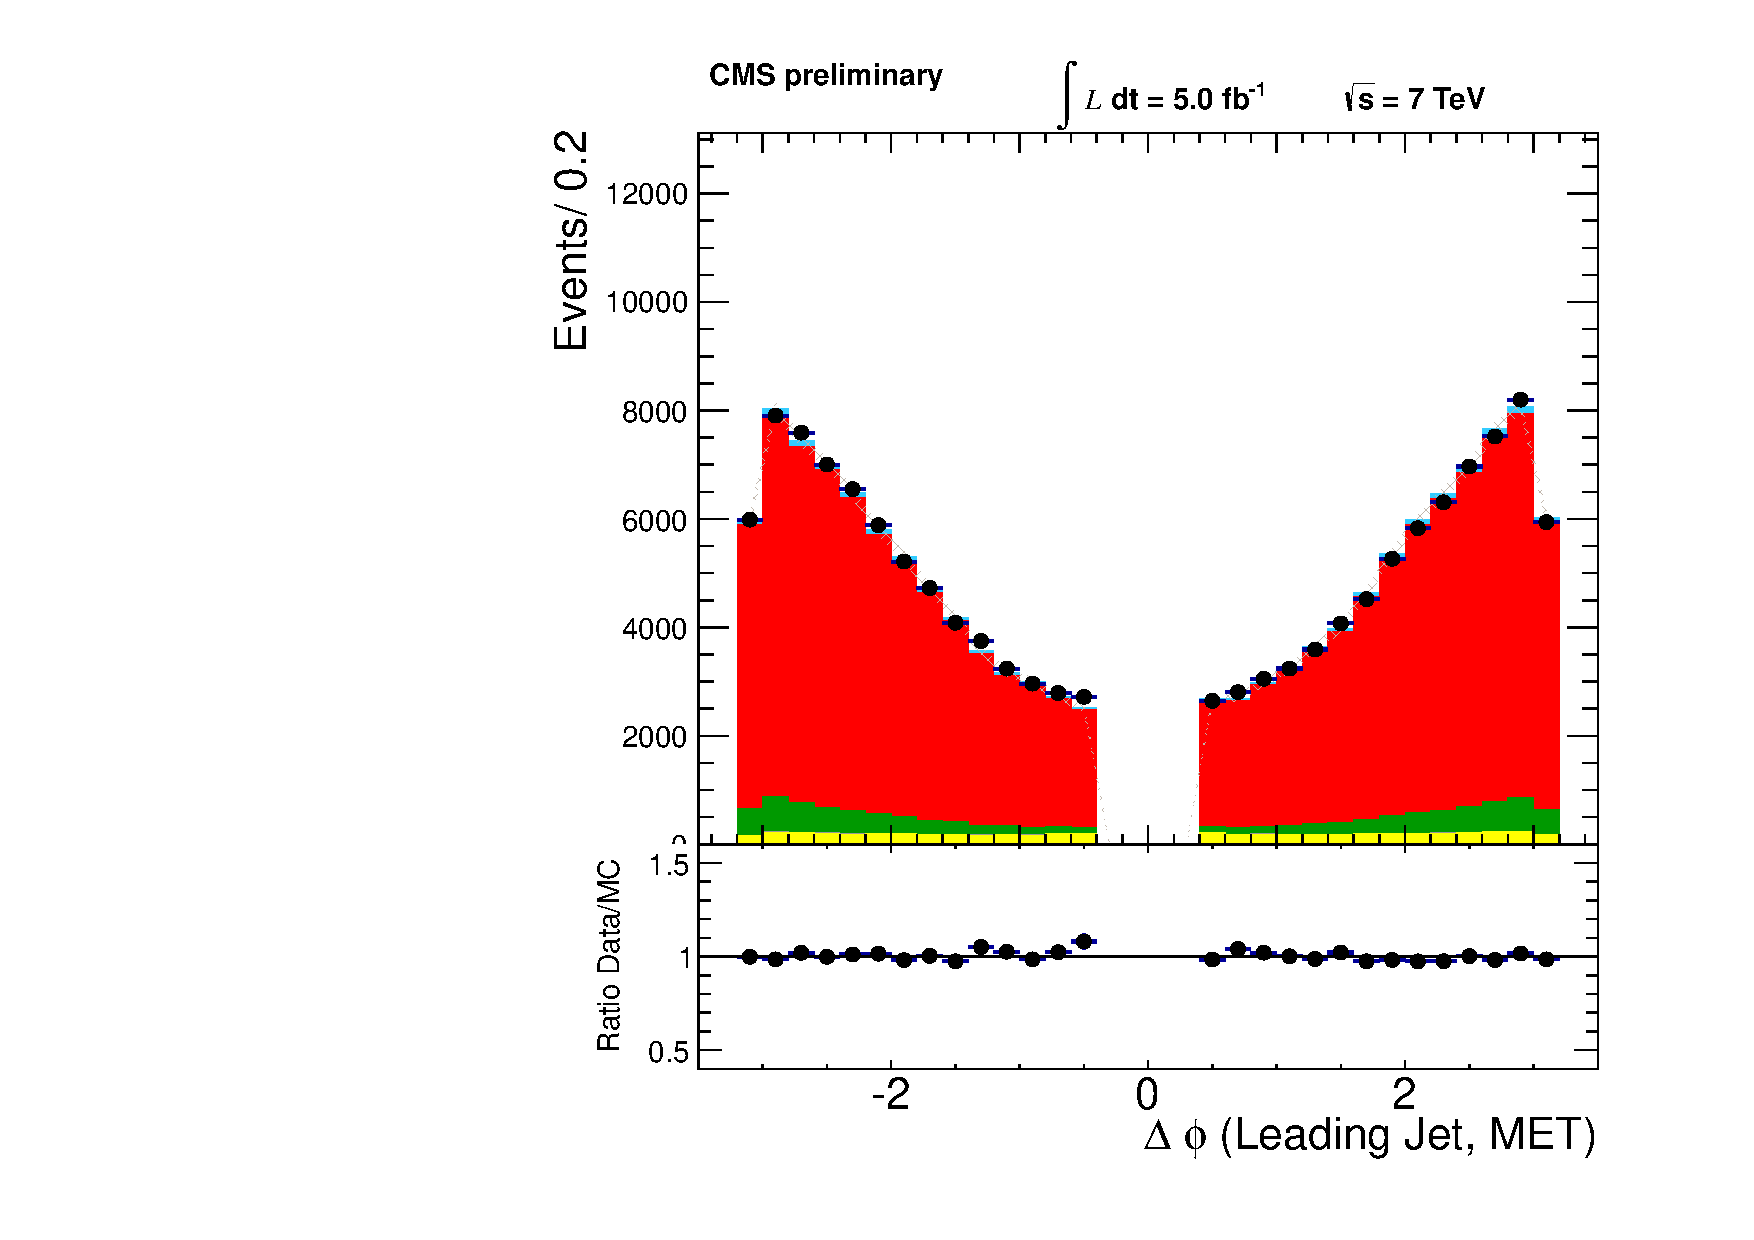
\includegraphics[width=0.49\textwidth]{figs/n-1_plots_mu/mu_deltaphi_jetldmet.pdf}
    \caption{Comparison of the distributions from data and MC of the
    dijet mass (left) and the $\Delta \phi $ between the leading jet and MET (right)
    for the muon+jets selection.}
\label{fig:mu_dijetmass}}
\end{figure}
\begin{figure}[h!t]
  {\centering
    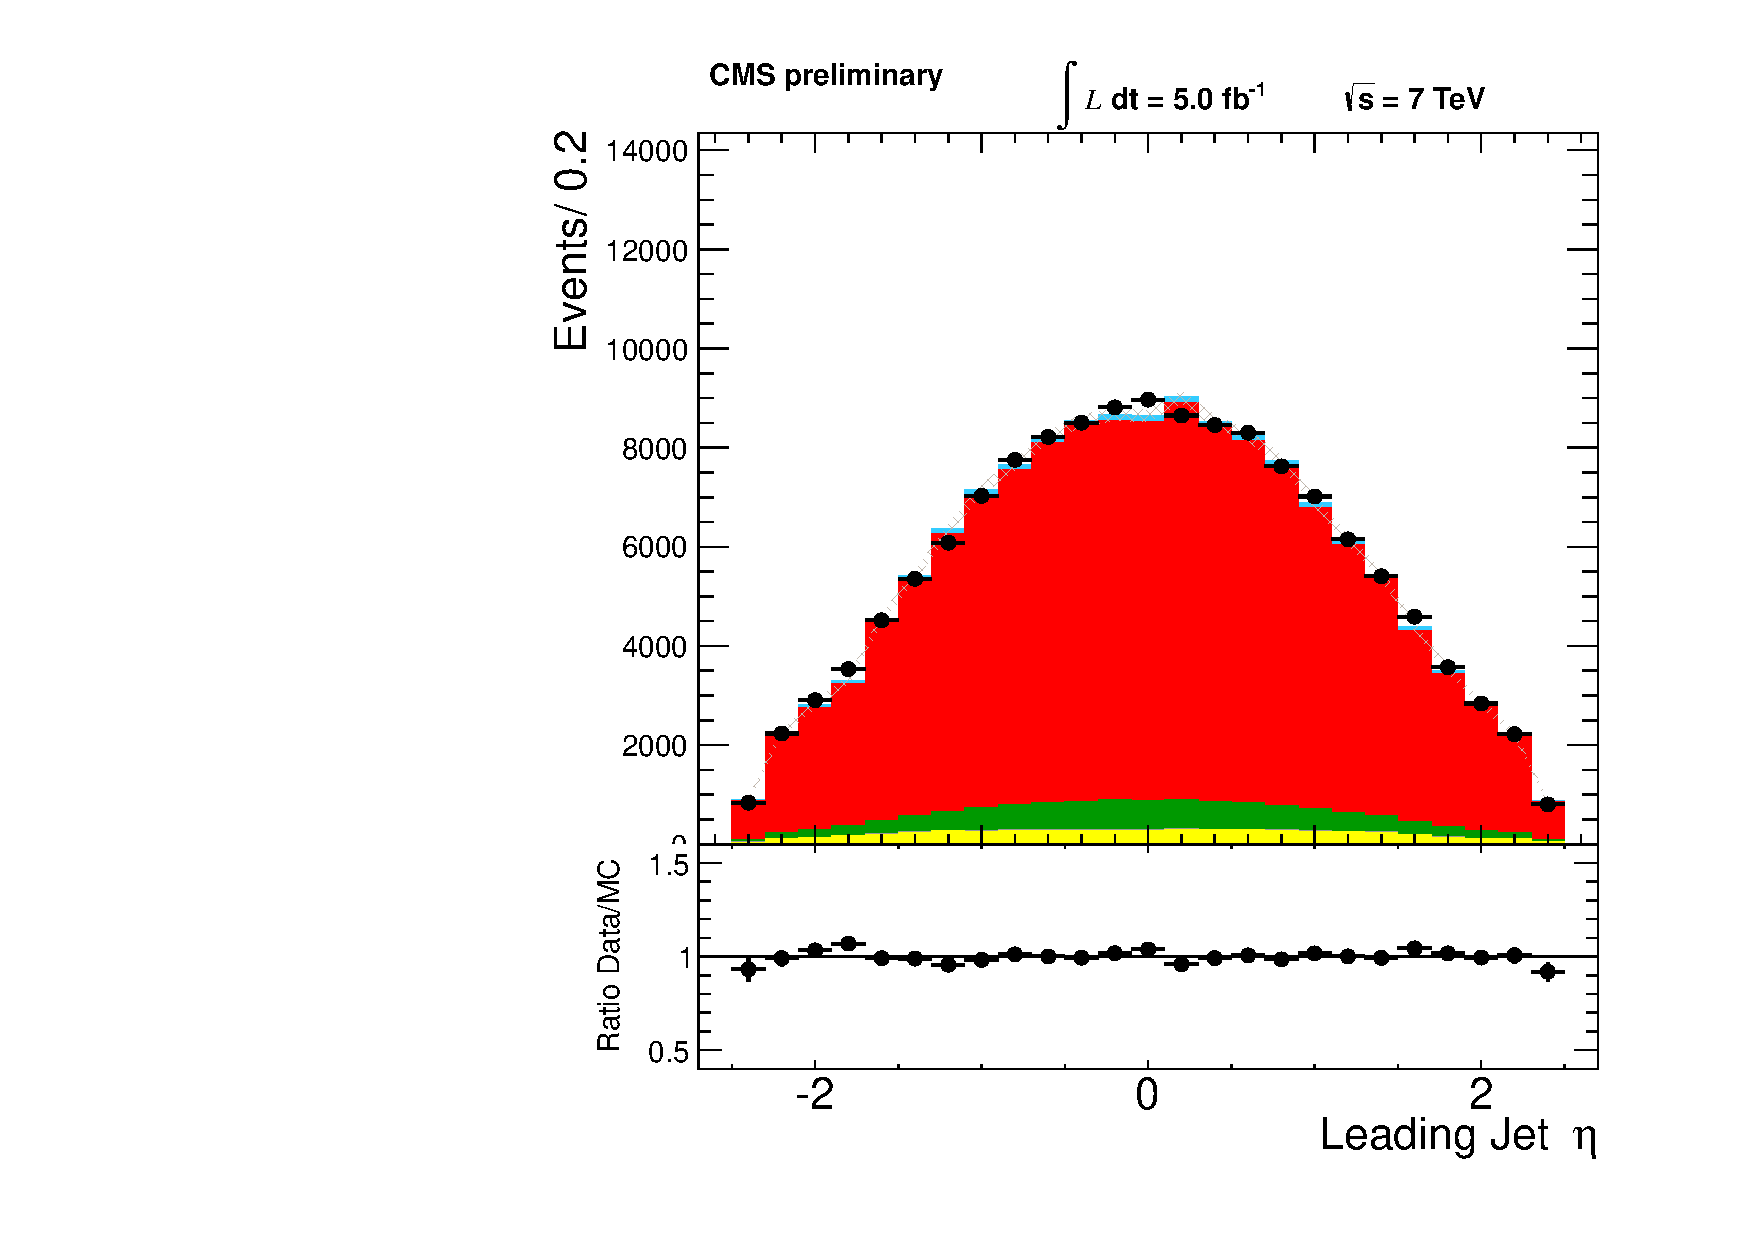
\includegraphics[width=0.49\textwidth]{figs/n-1_plots_mu/mu_jetld_eta.pdf}
    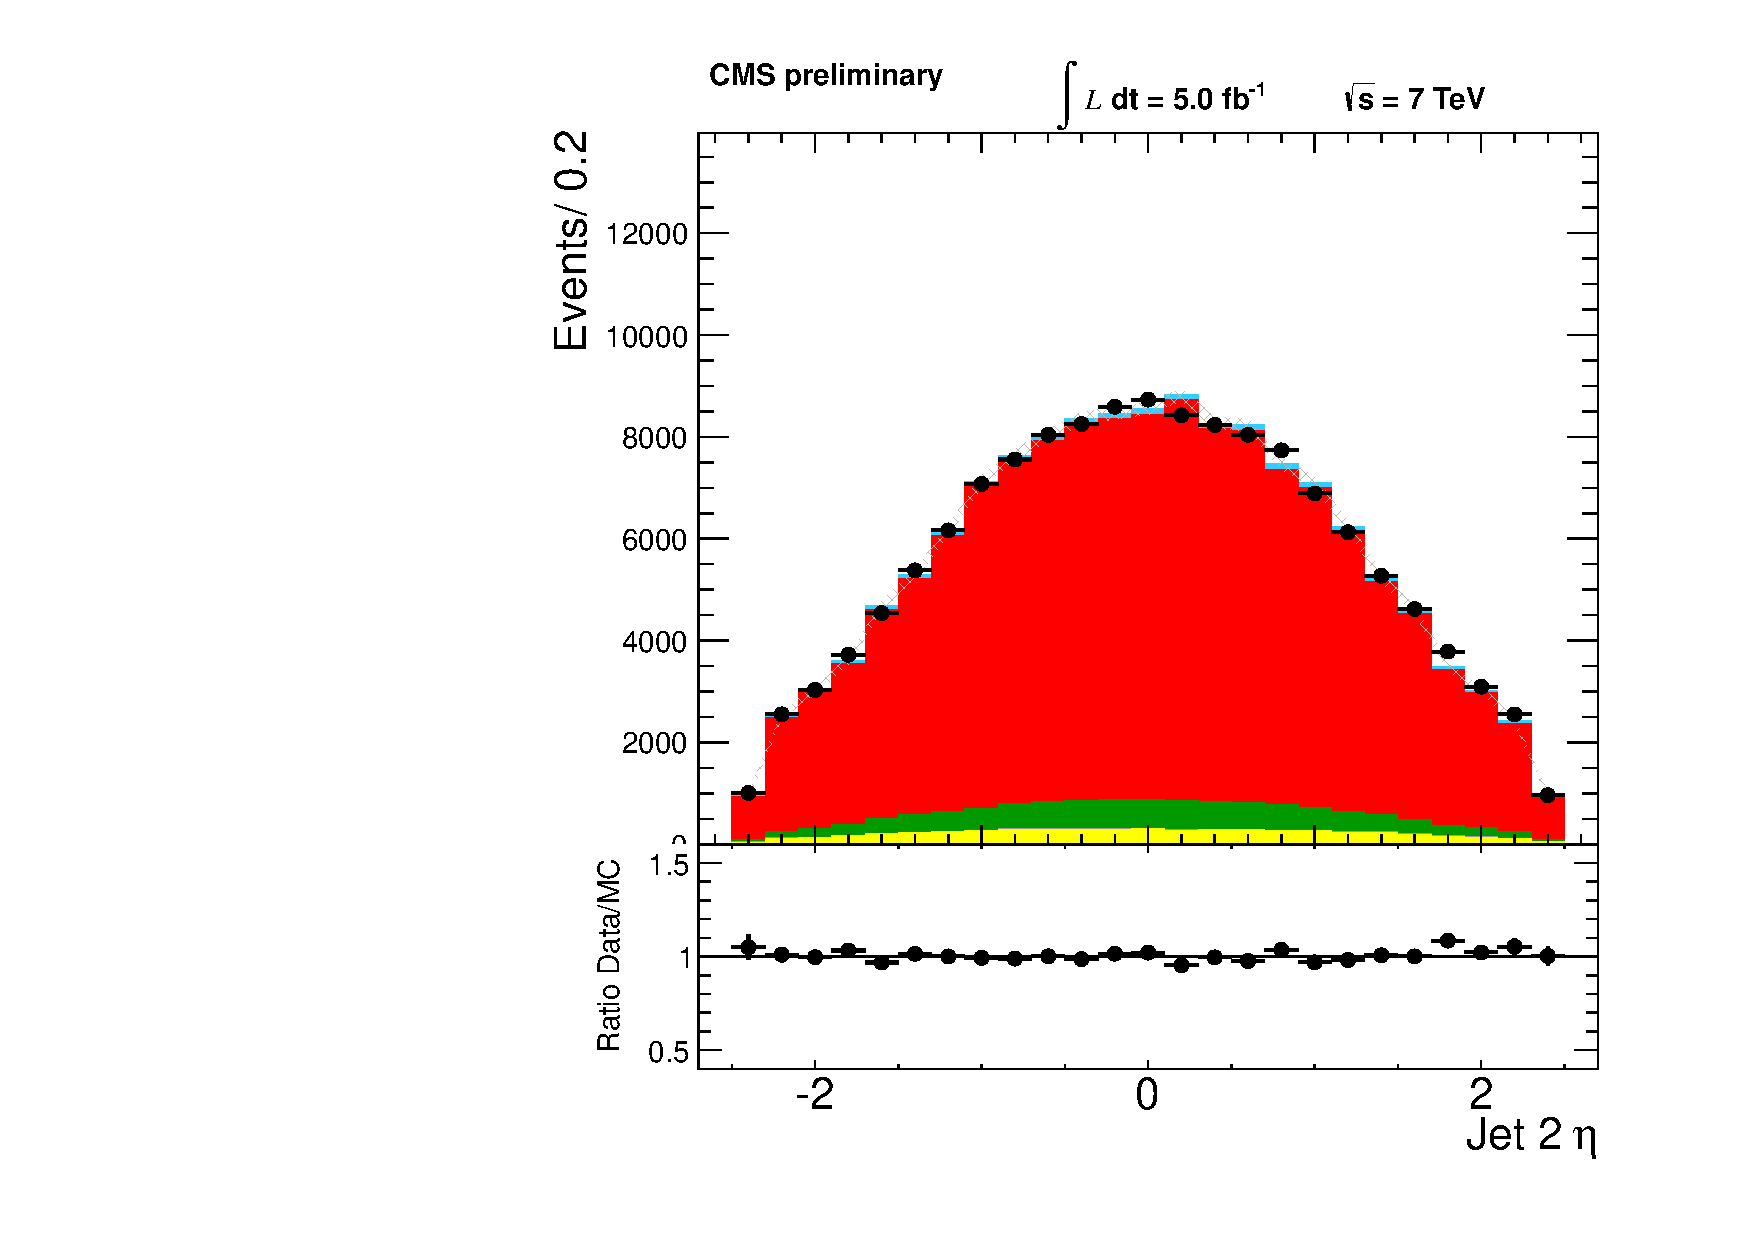
\includegraphics[width=0.49\textwidth]{figs/n-1_plots_mu/mu_jetnt_eta.pdf}
    \caption{Comparison of the leading jet $\eta $ (left) and the
    second leading jet $\eta $ (right) distributions from data and MC
    for the muon+jets selection. }
\label{fig:mu_jet_eta}}
\end{figure}
%%%%%%%%%%%%%%%%%%%%%%%%%%%%
\begin{figure}[h!t]
  {\centering
    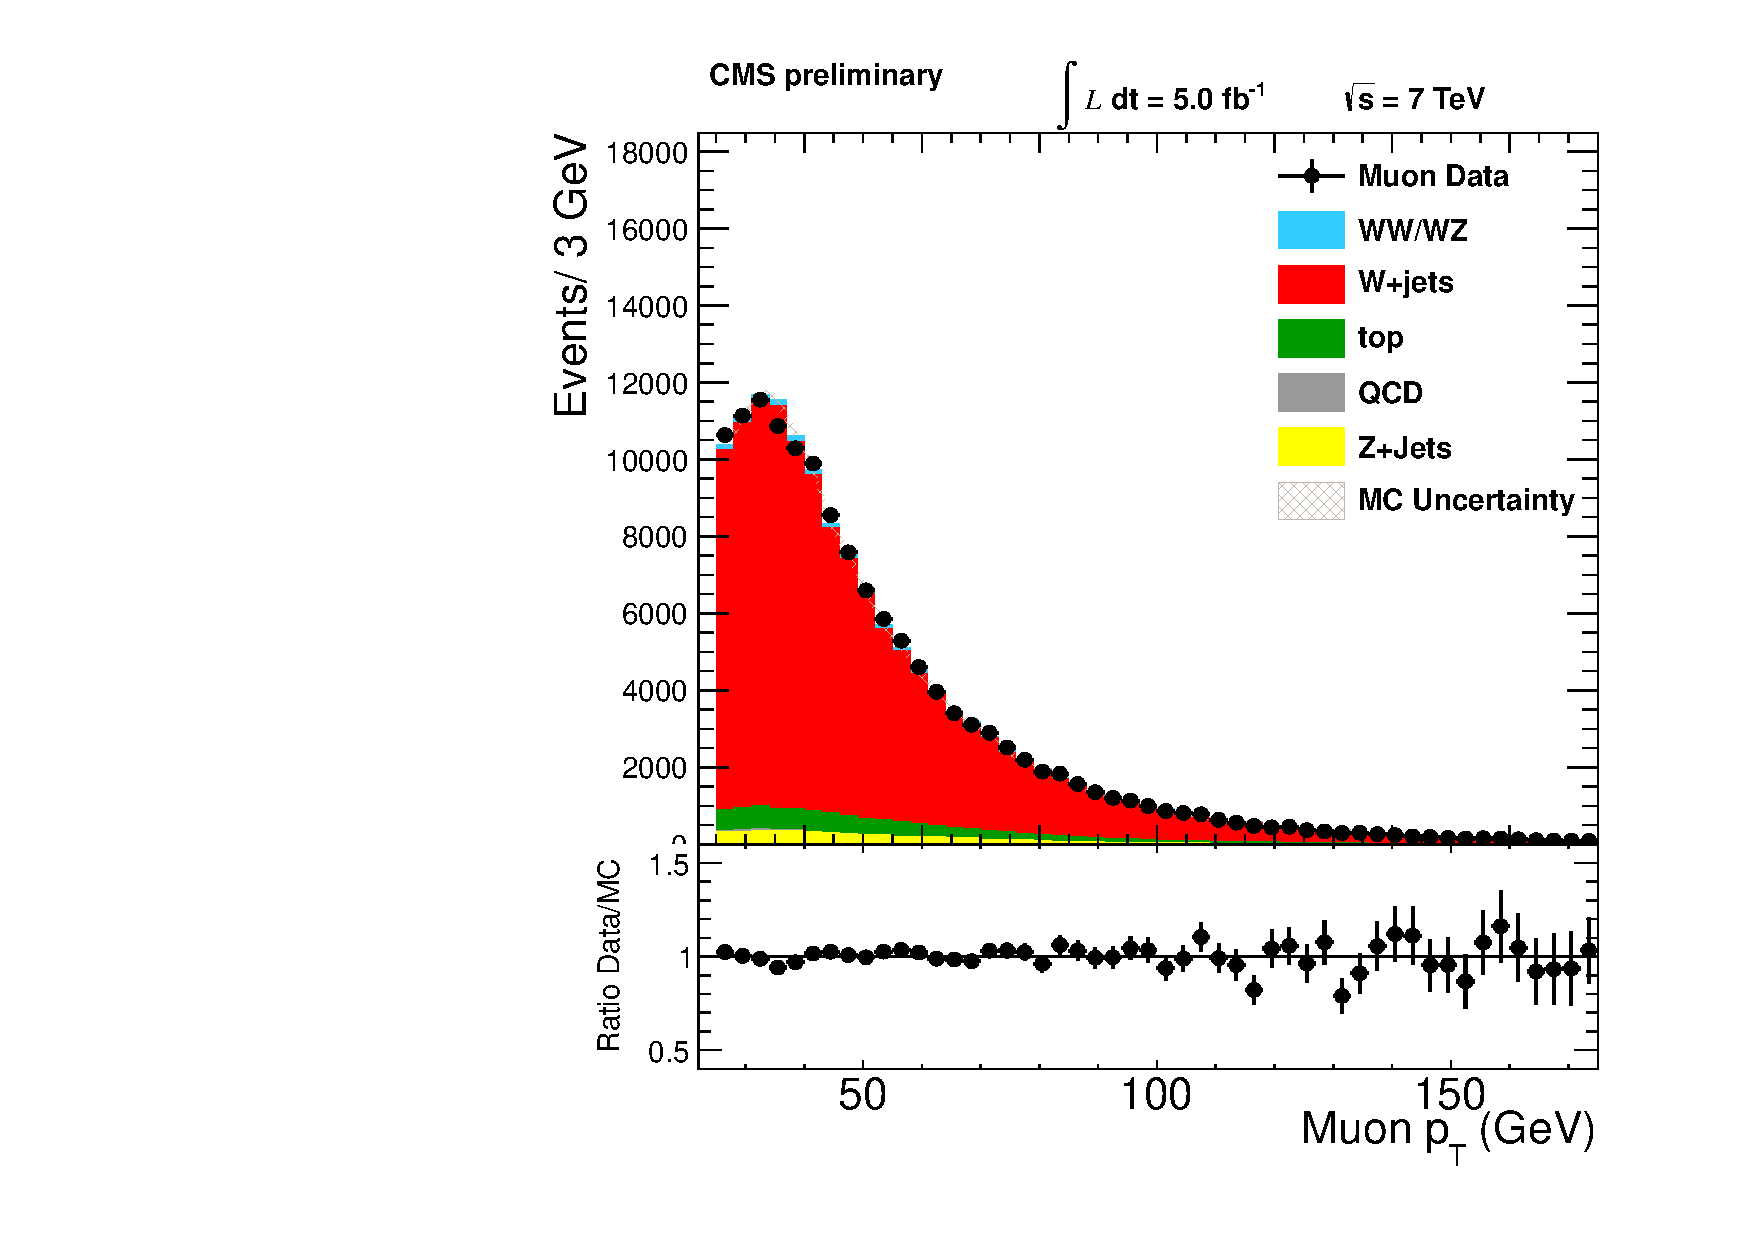
\includegraphics[width=0.49\textwidth]{figs/n-1_plots_mu/mu_W_muon_pt.pdf}
    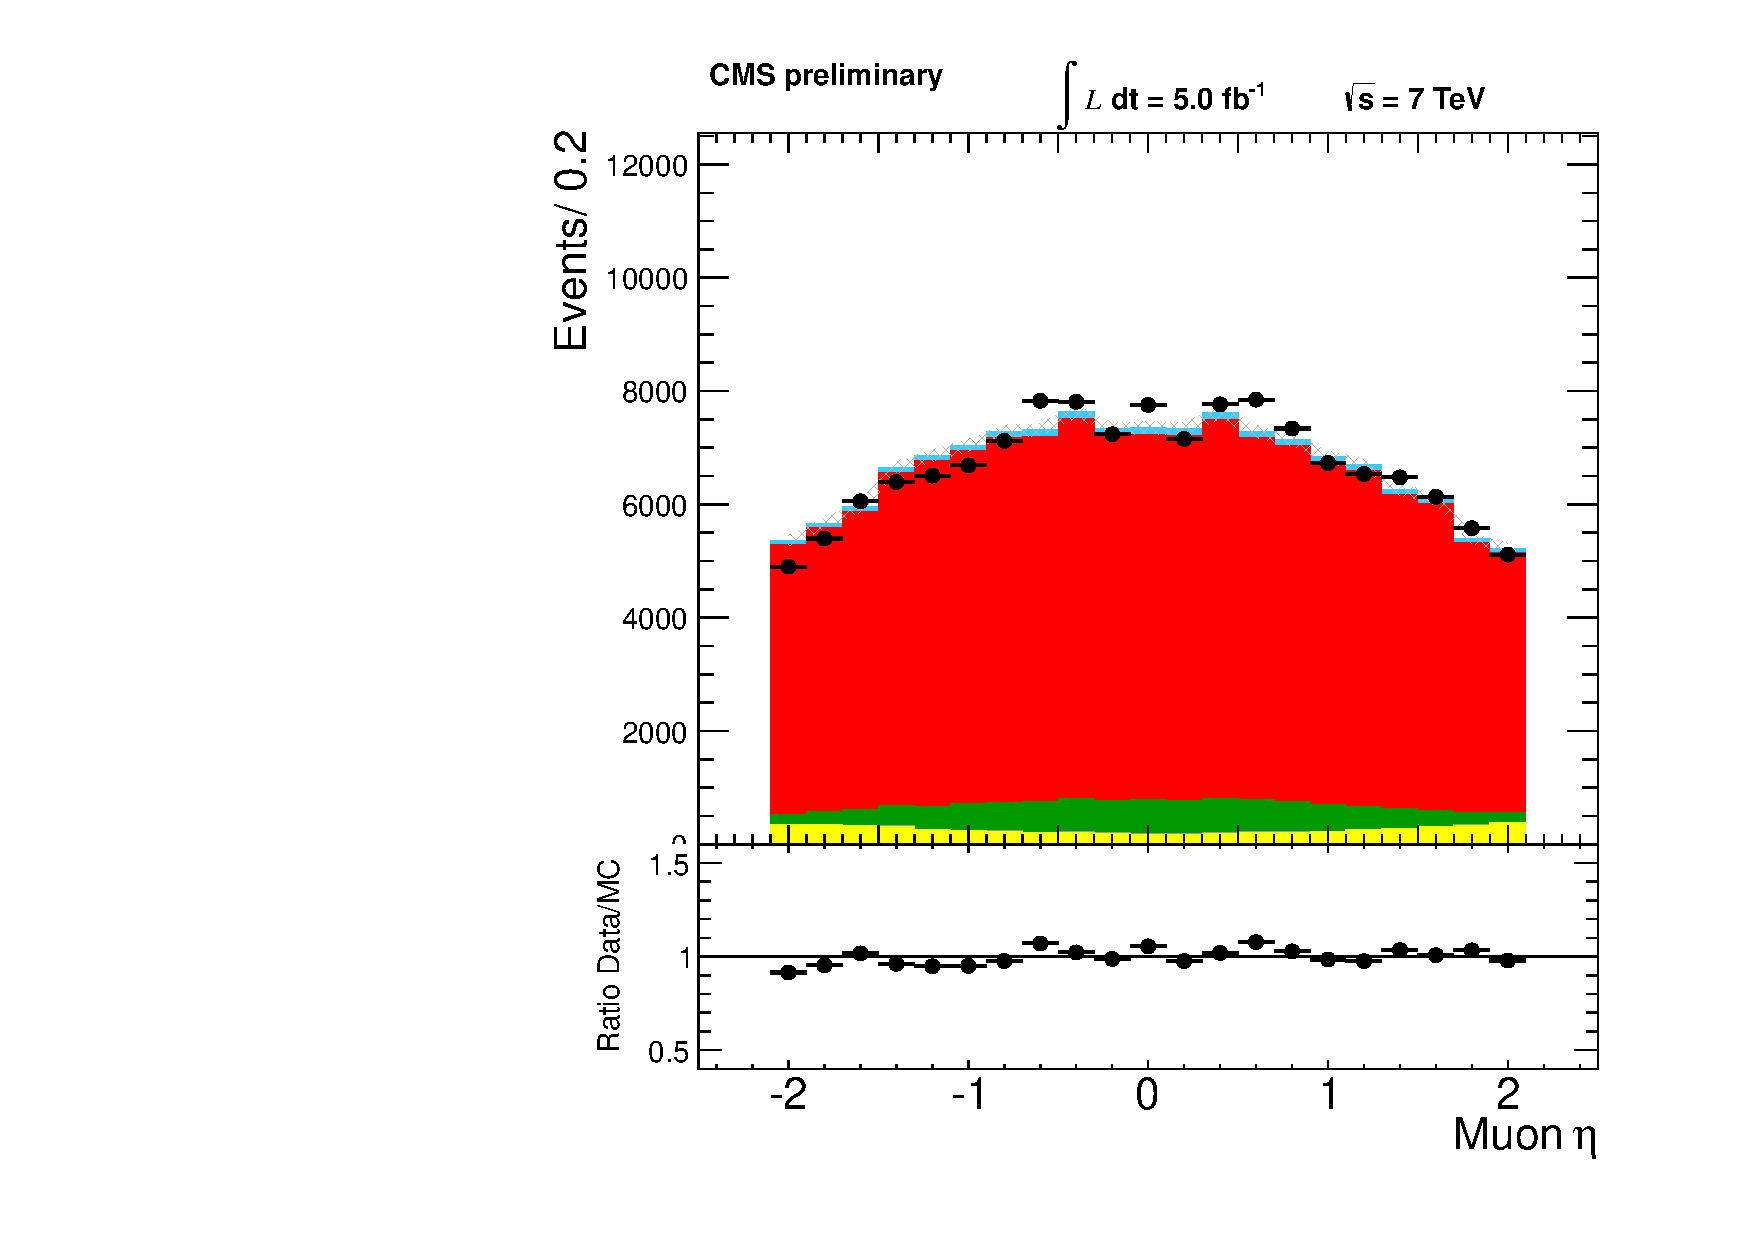
\includegraphics[width=0.49\textwidth]{figs/n-1_plots_mu/mu_W_muon_eta.pdf}
    \caption{Comparison of the muon $p_{T} $ (left) and the muon
      $\eta $ (right) distributions from data and MC for the muon+jets selection.
      }
    \label{fig:mu_muon}}
\end{figure}
%%%%%%%%%%%%%%%%%%%%%%%%%%%%
\begin{figure}[h!t]
  {\centering
    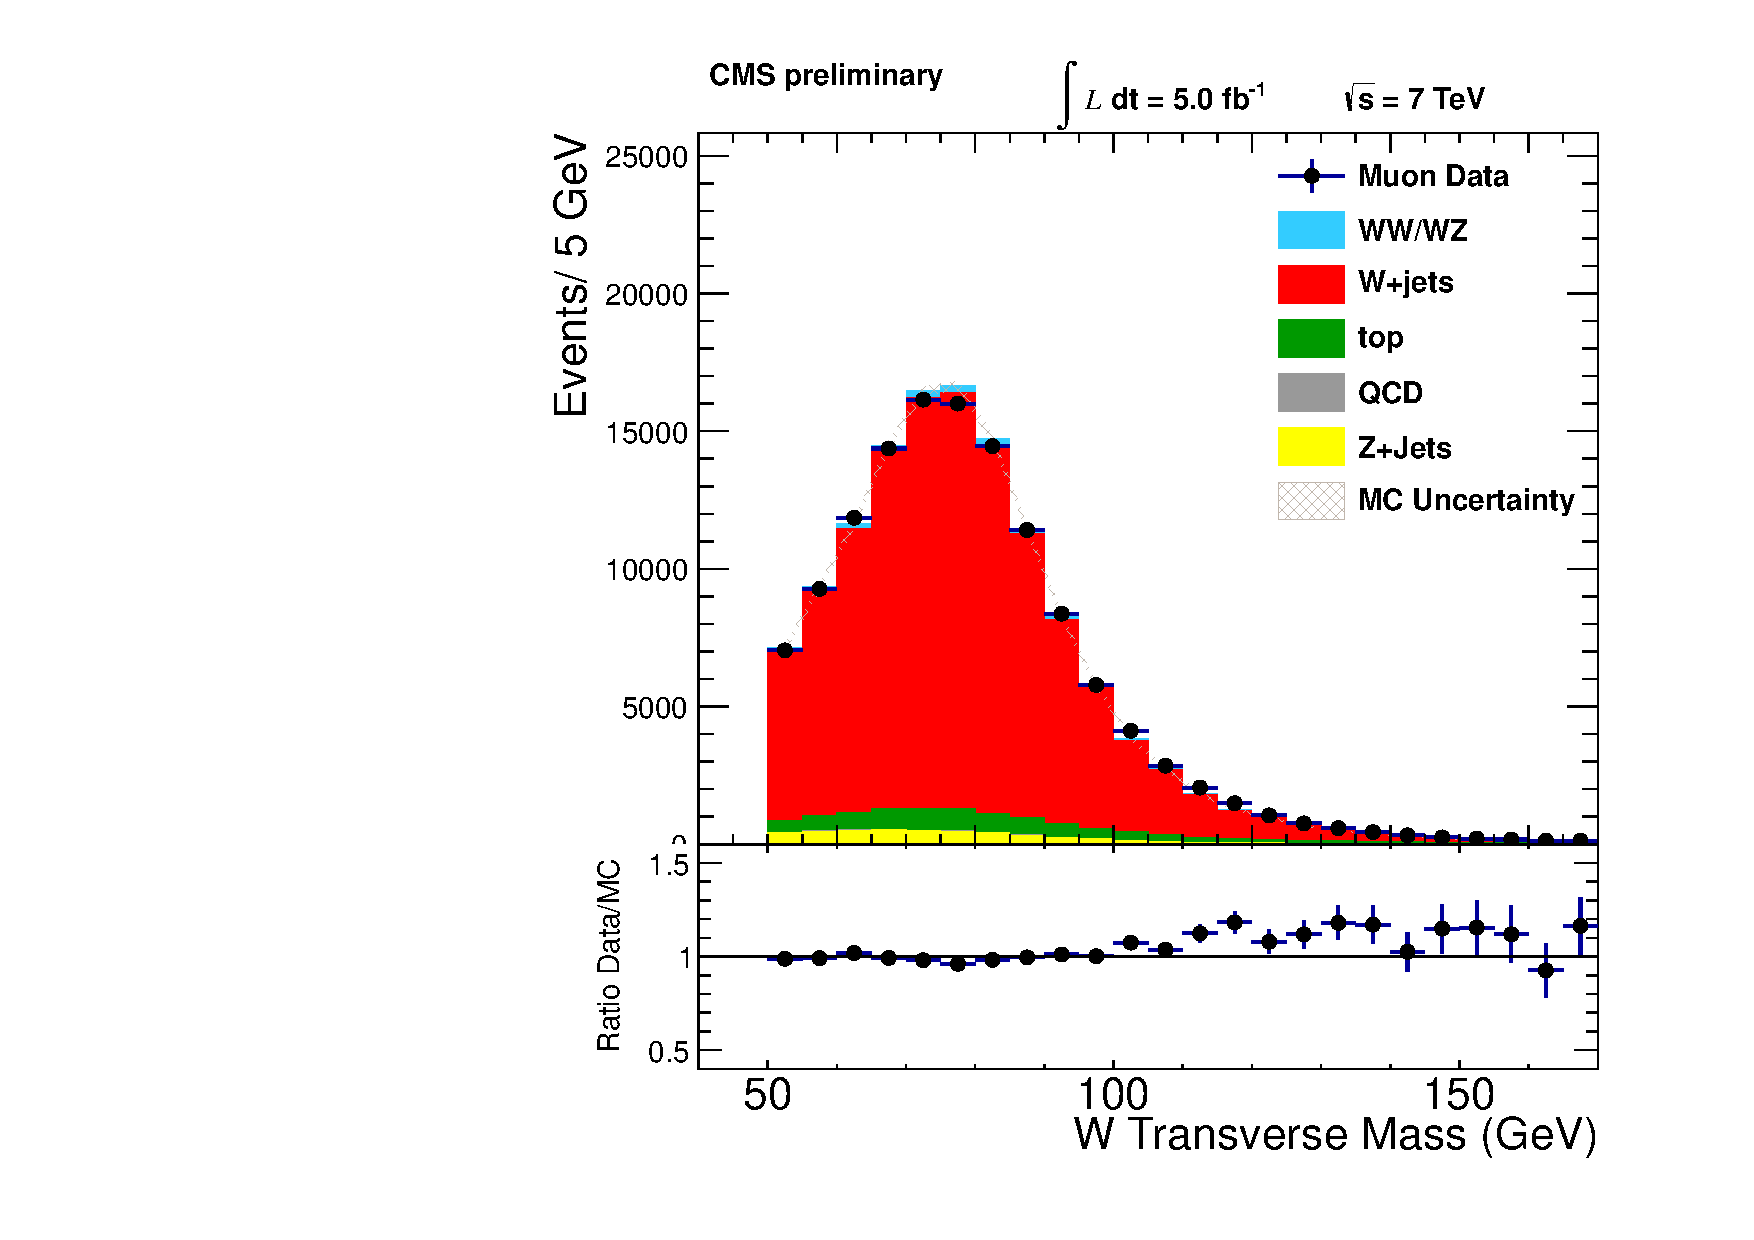
\includegraphics[width=0.49\textwidth]{figs/n-1_plots_mu/mu_W_mt.pdf}
    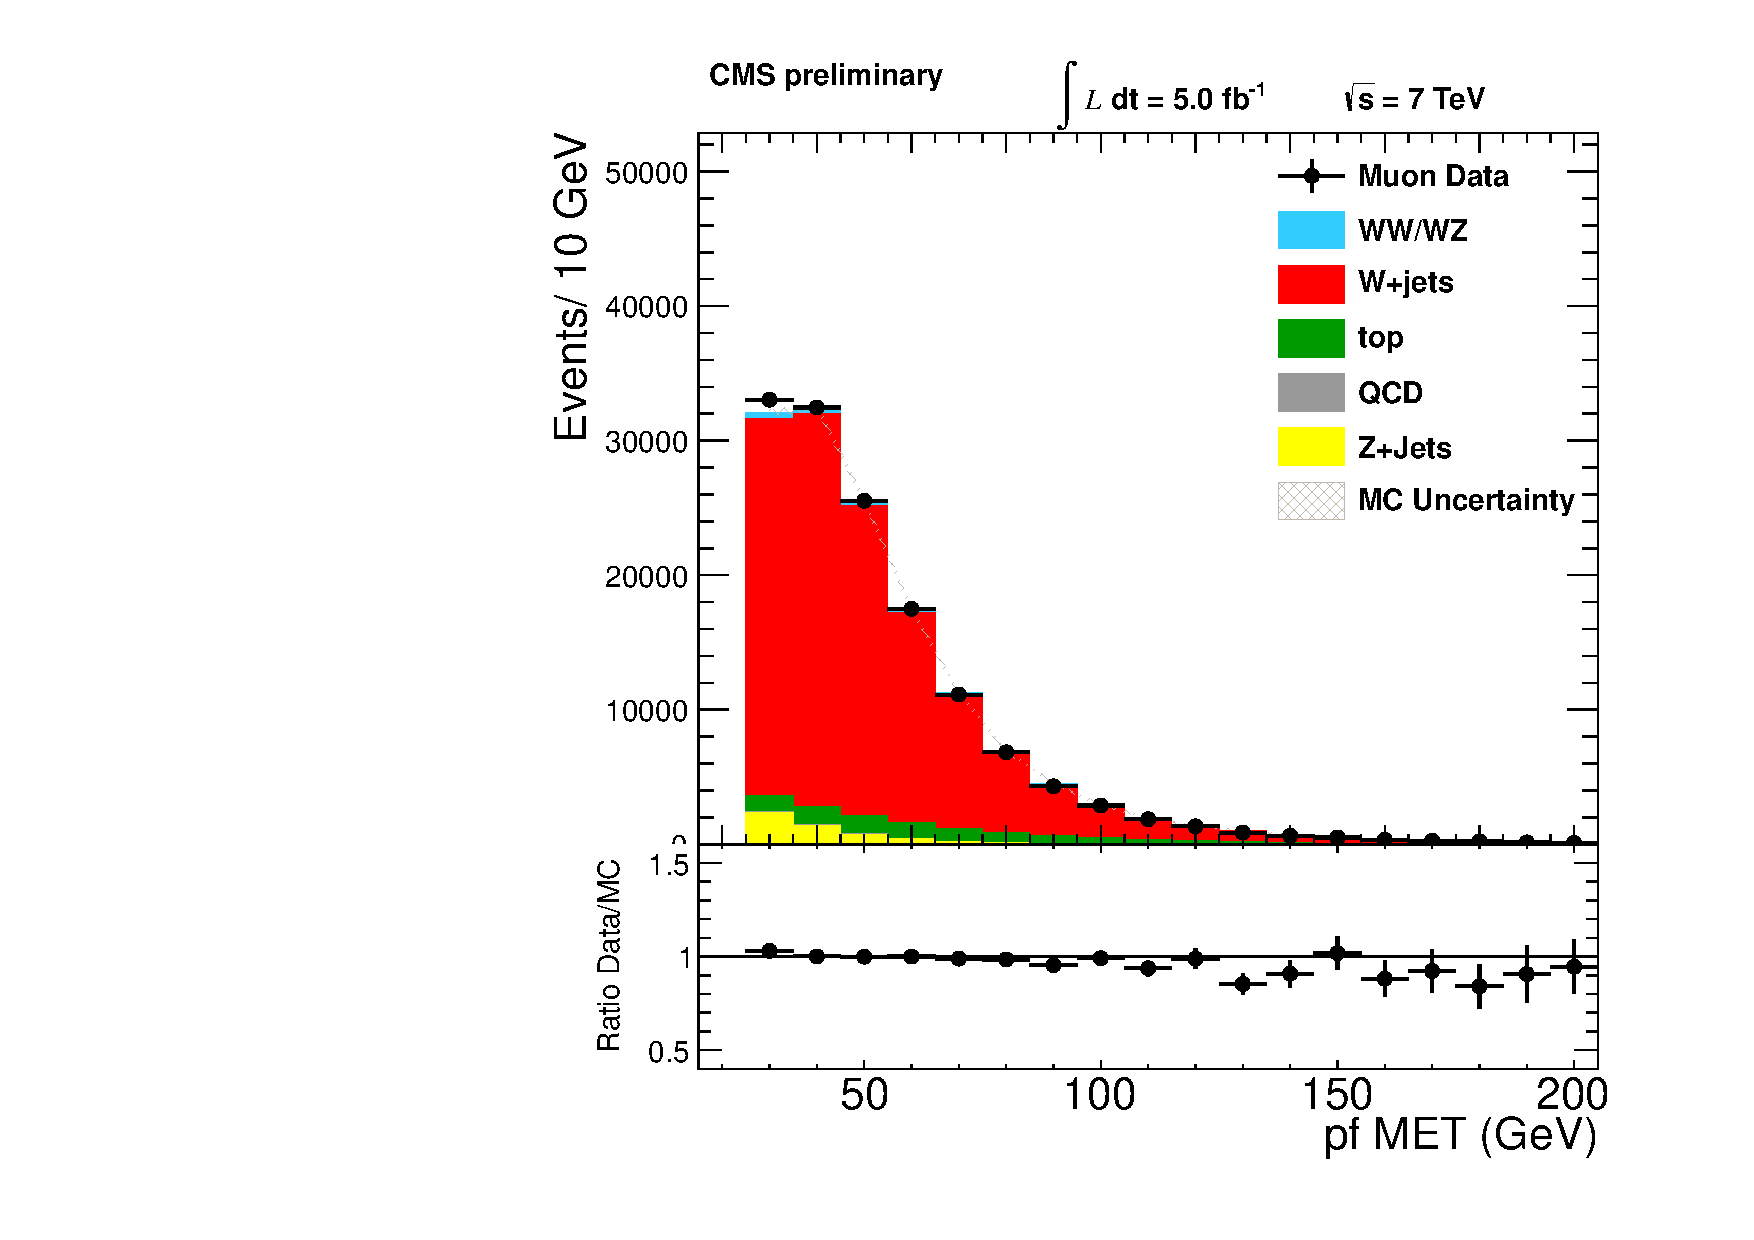
\includegraphics[width=0.49\textwidth]{figs/n-1_plots_mu/mu_event_met_pfmet.pdf}
    \caption{Comparison of the distributions from data and MC of the
     transverse mass of the muon / MET system (left) and the MET (right)
    for the muon+jets selection. 
    }
    \label{fig:mu_W_Mt}}
\end{figure}
%%%%%%%%%%%%%%%%%%%%%%%%%%%%
%%%%%%%%%%%%%%%%%%%%%%%%%%%%
\begin{figure}[h!t]
  {\centering
    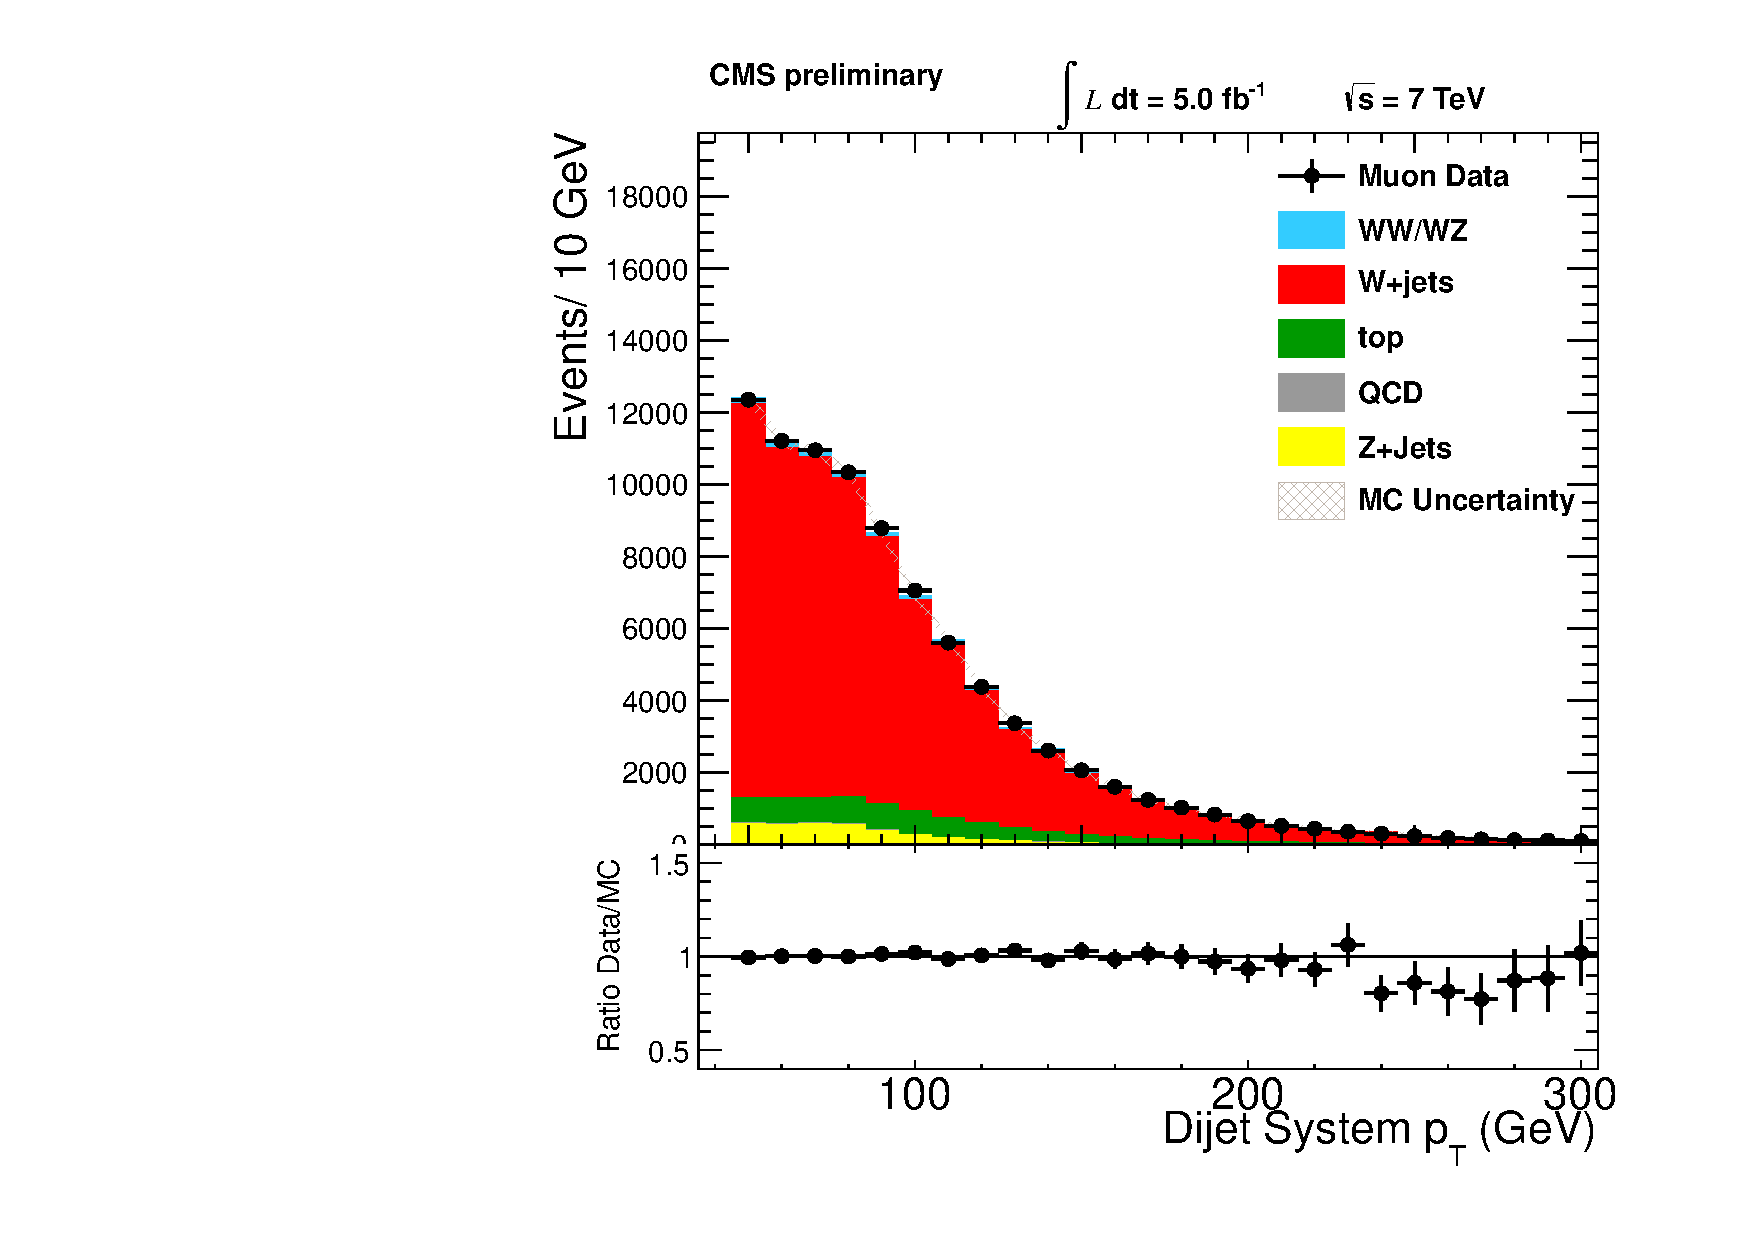
\includegraphics[width=0.49\textwidth]{figs/n-1_plots_mu/mu_dijet_pt.pdf}
    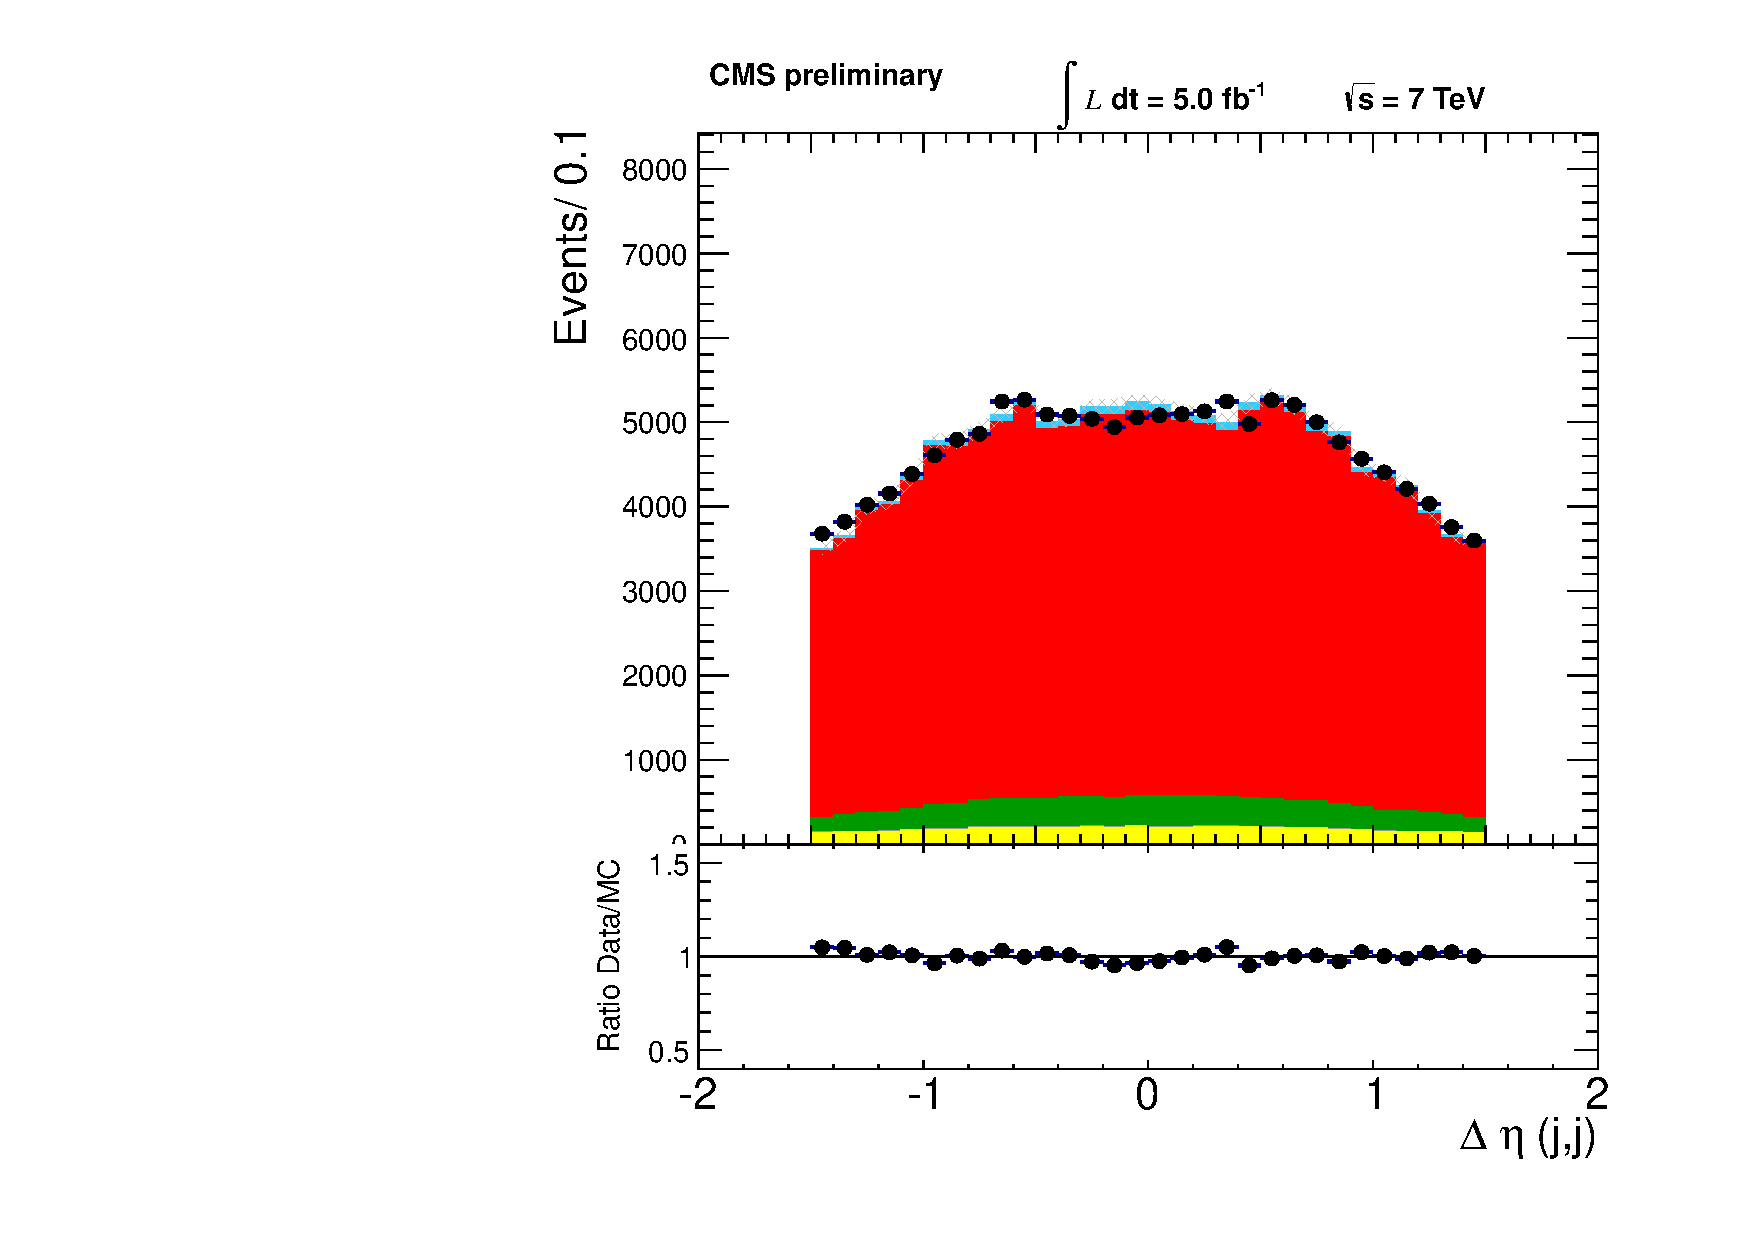
\includegraphics[width=0.49\textwidth]{figs/n-1_plots_mu/mu_deltaeta_jj.pdf}
    \caption{Comparison of the distributions from
      data and MC of the dijet system $p_{T}$ (left)
      and the $\eta $ separation between the two jets (right) for the muon+jets selection. 
      }
    \label{fig:mu_dijet}}
\end{figure}
%%%%%%%%%%%%%%%%%%%%%%%%%%%%
%%%%%%%%%%%%%%%%%%%%%%%%%%%%
\begin{figure}[h!t]
  {\centering
    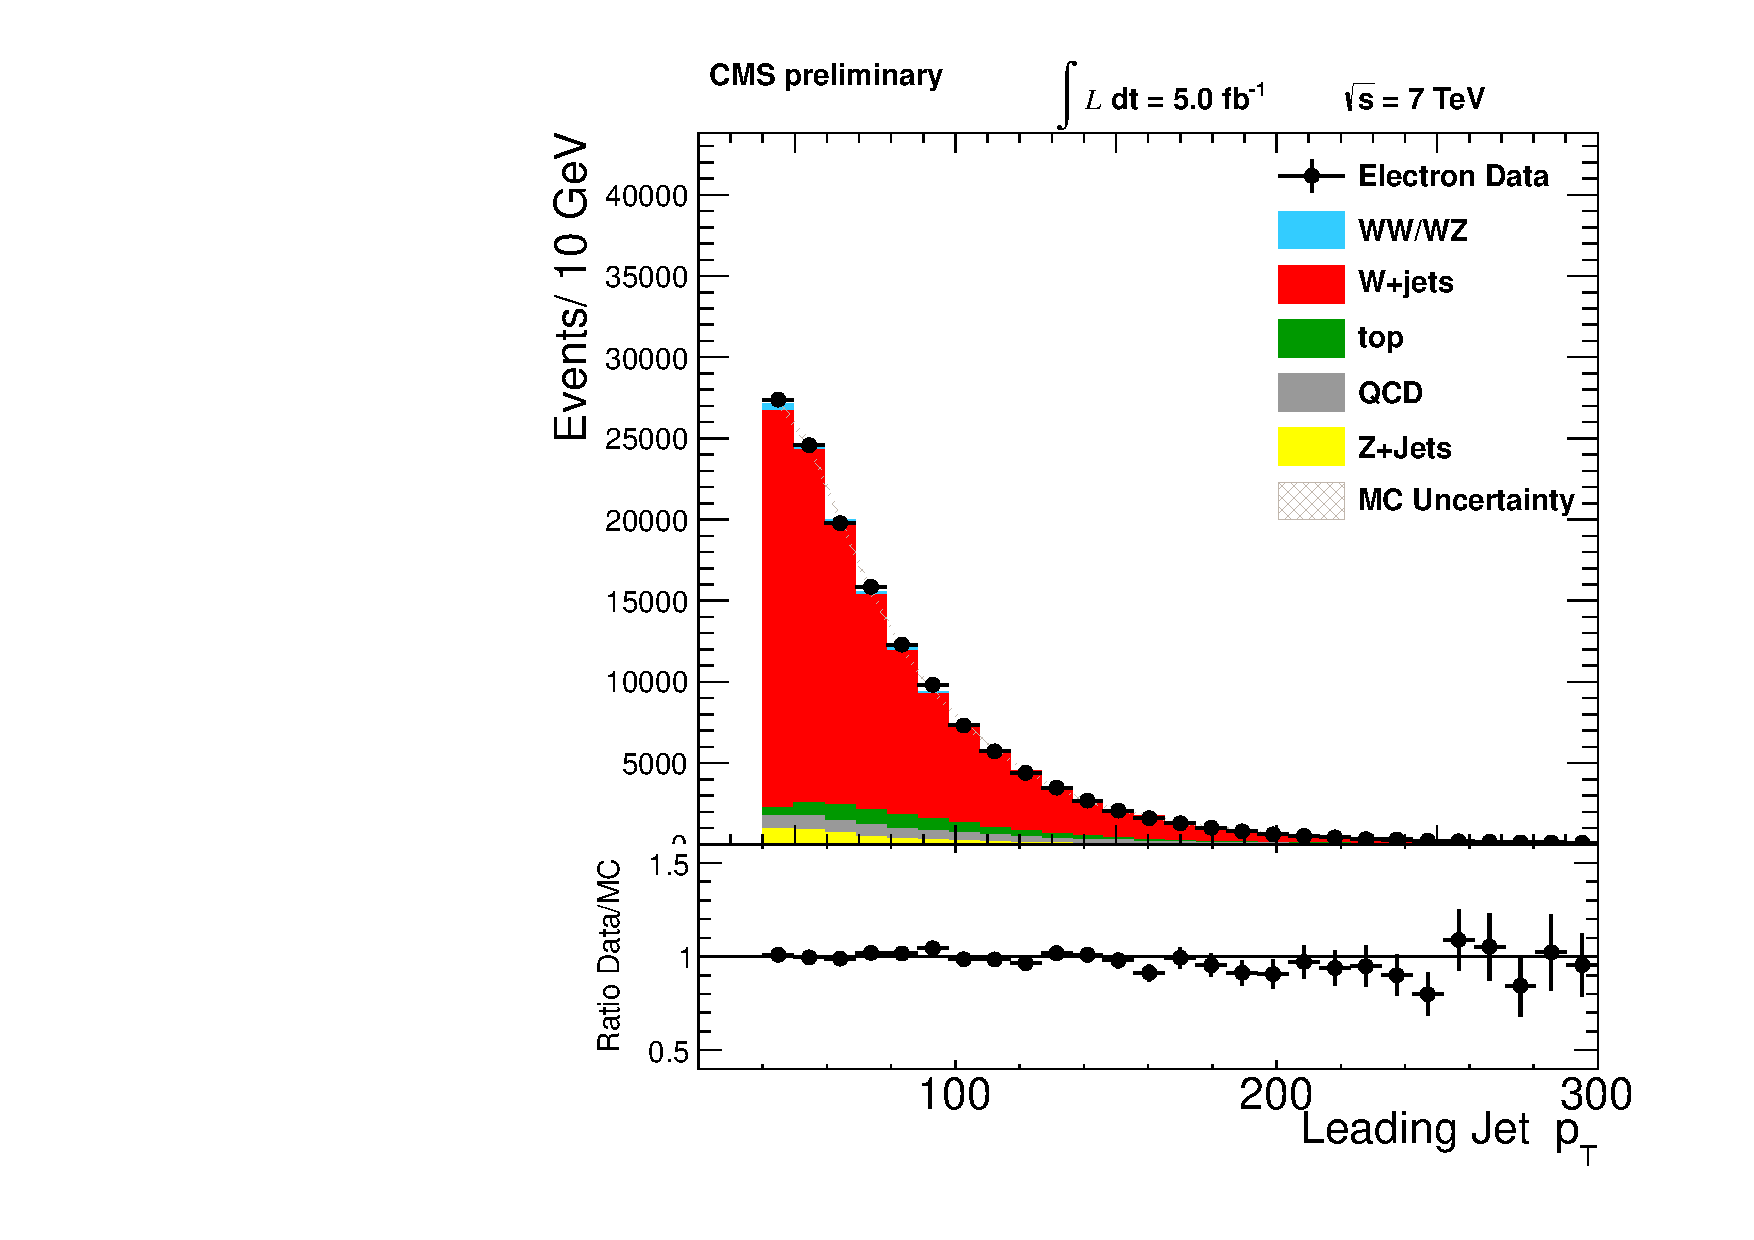
\includegraphics[width=0.49\textwidth]{figs/n-1_plots_el/el_jetld_pt.pdf}
    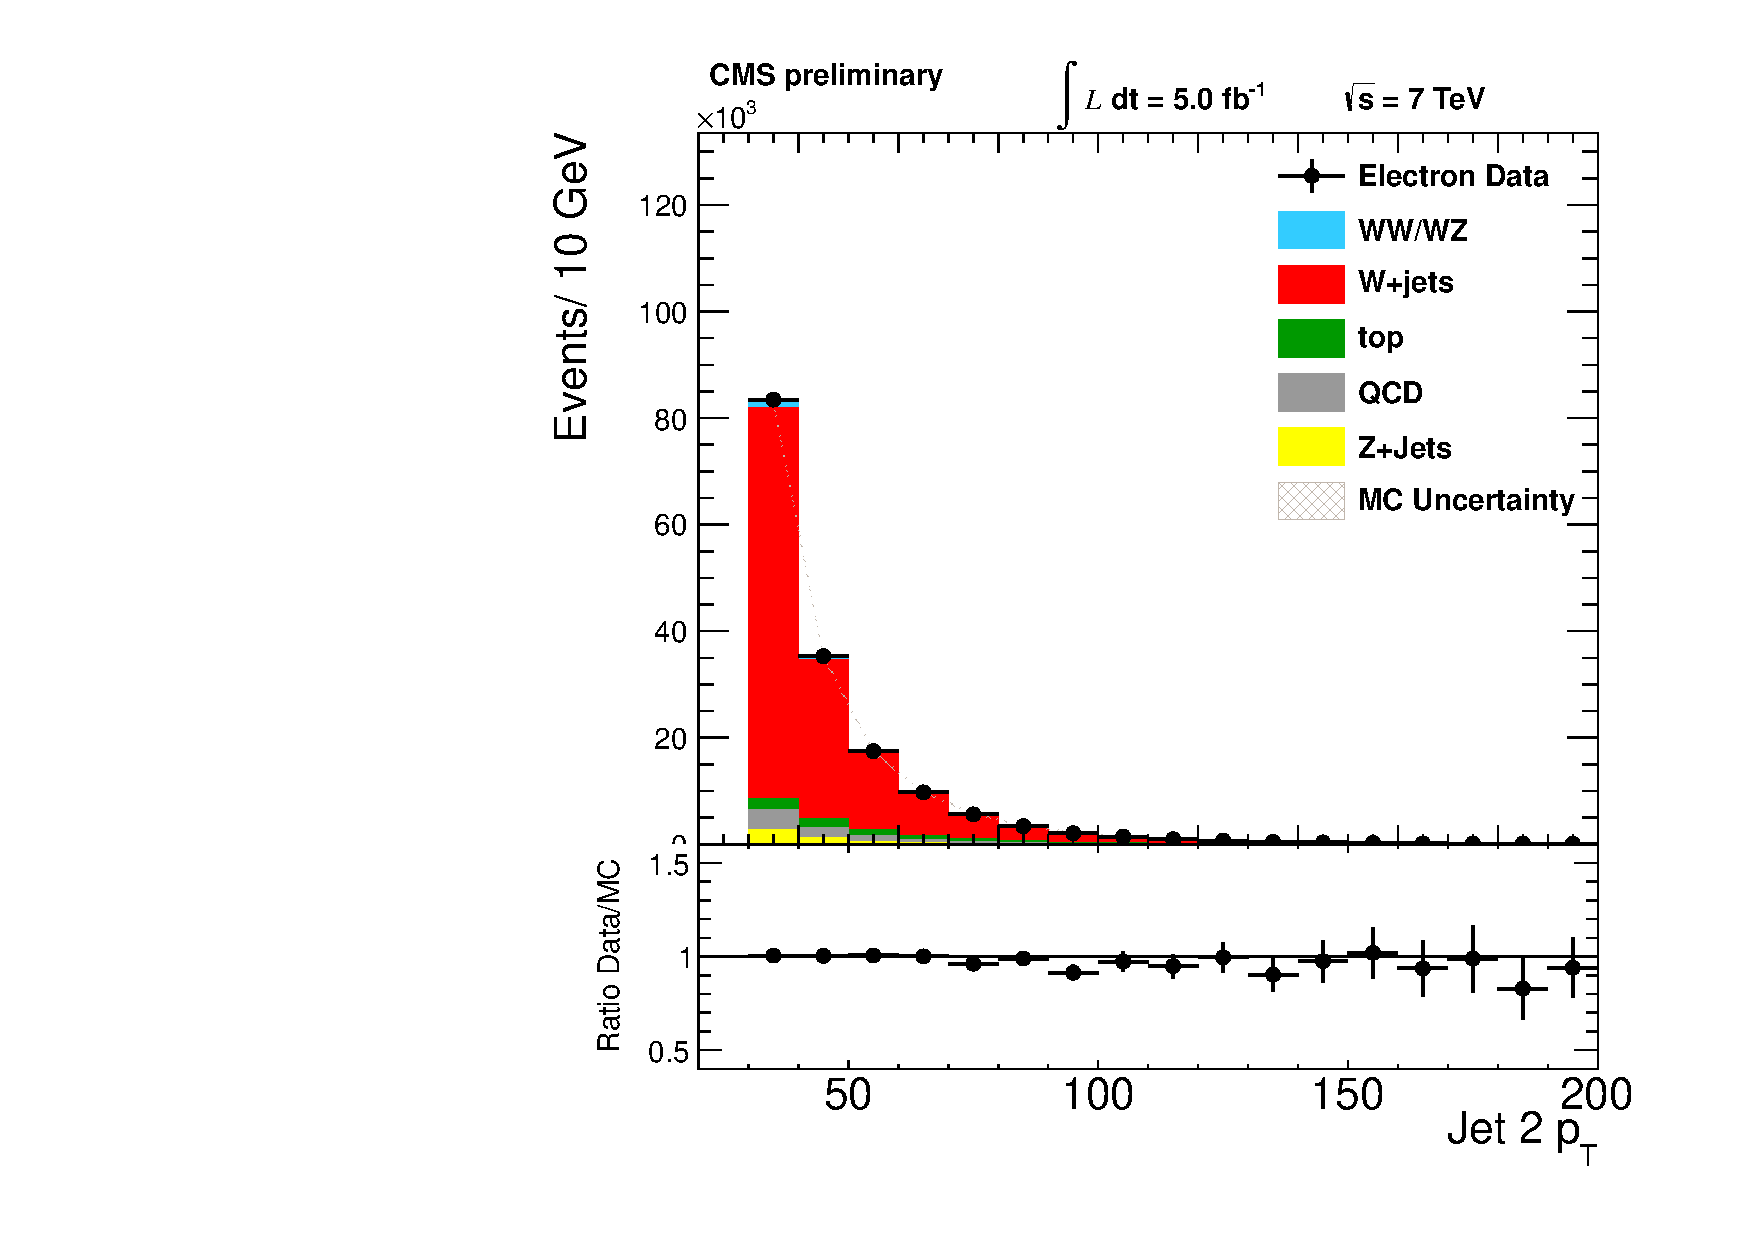
\includegraphics[width=0.49\textwidth]{figs/n-1_plots_el/el_jetnt_pt.pdf}
    \caption{Comparison of the leading jet $p_{T} $ (left) and the
      second leading jet $p_{T} $ (right) distributions from data and MC
      for the electron+jets selection. 
      }
    \label{fig:elec_jet_pt}}
\end{figure}
%%%%%%%%%%%%%%%%%%%%%%%%%%%%
\begin{figure}[h!t]
  {\centering
    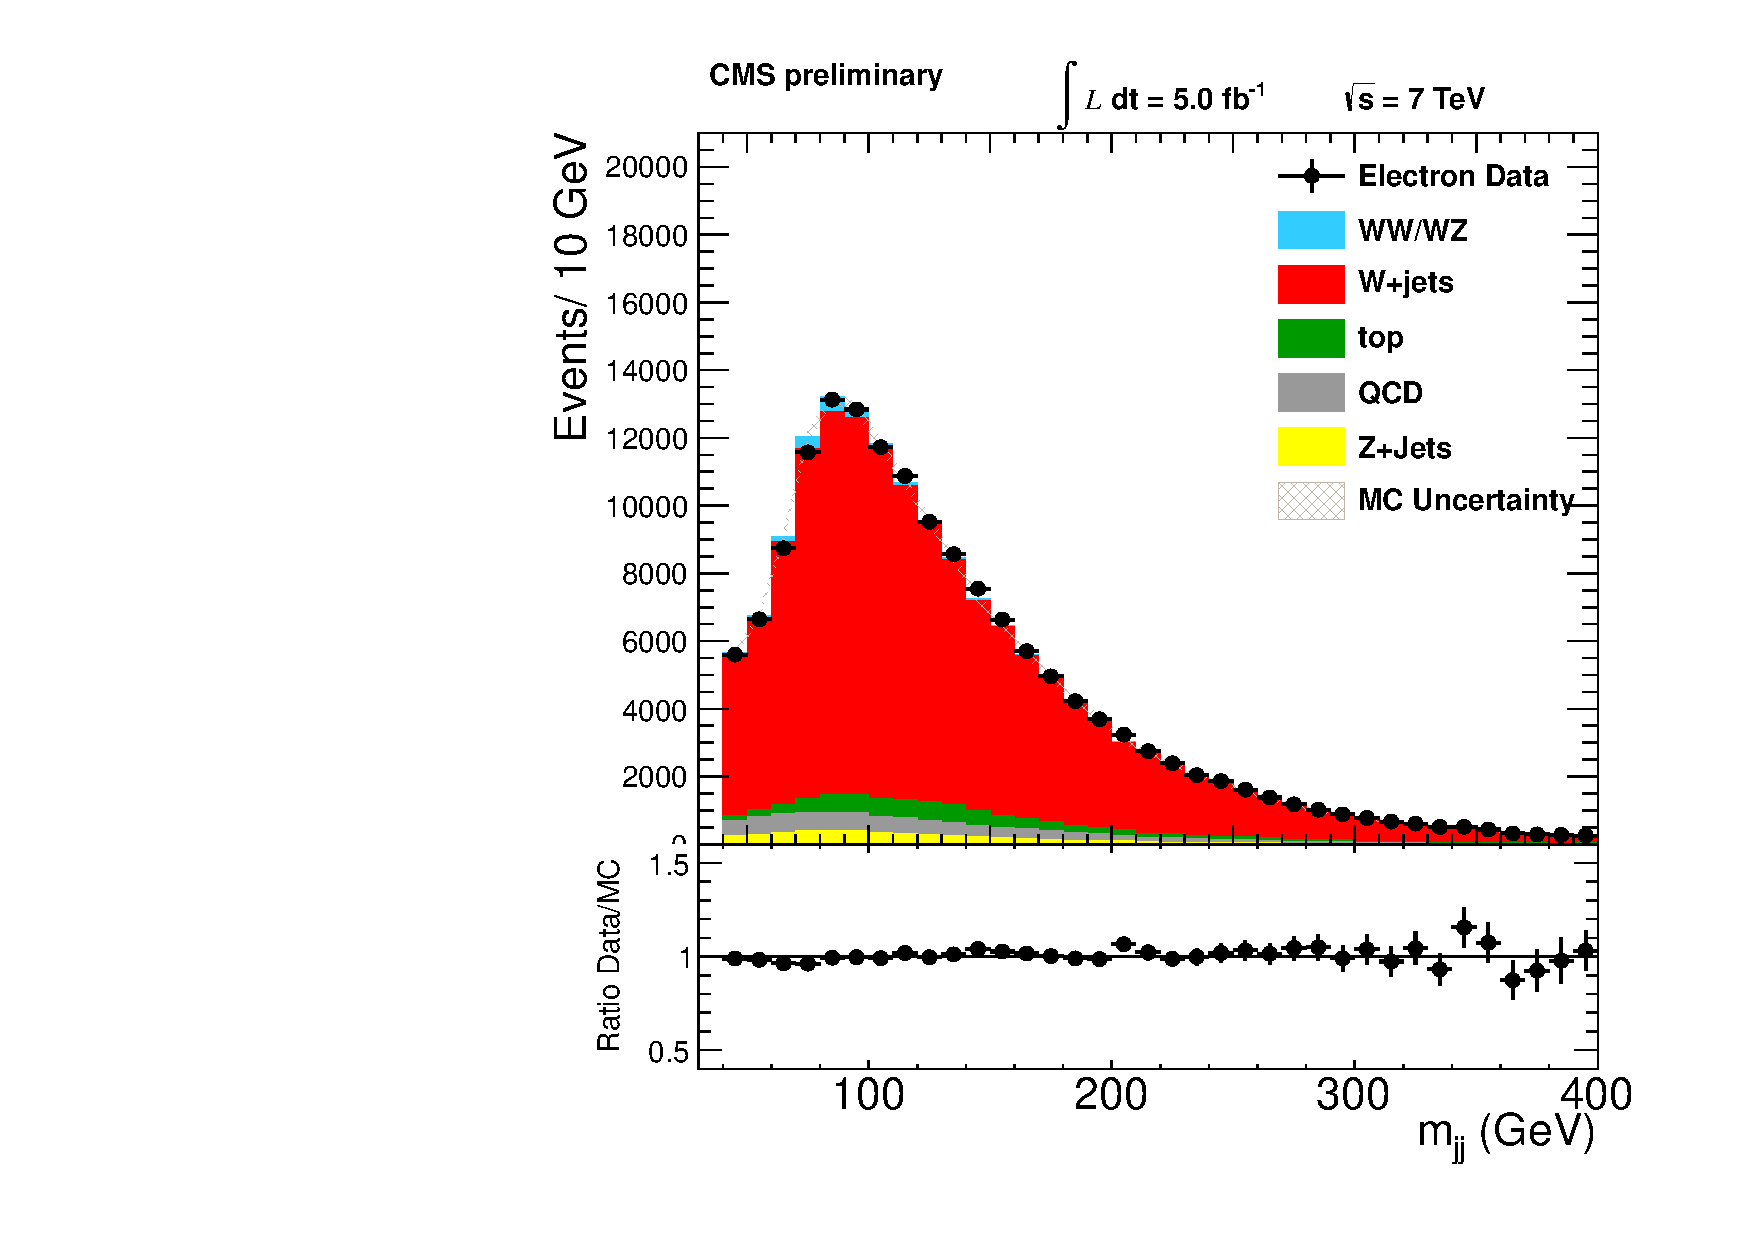
\includegraphics[width=0.49\textwidth]{figs/n-1_plots_el/el_mjj.pdf}
    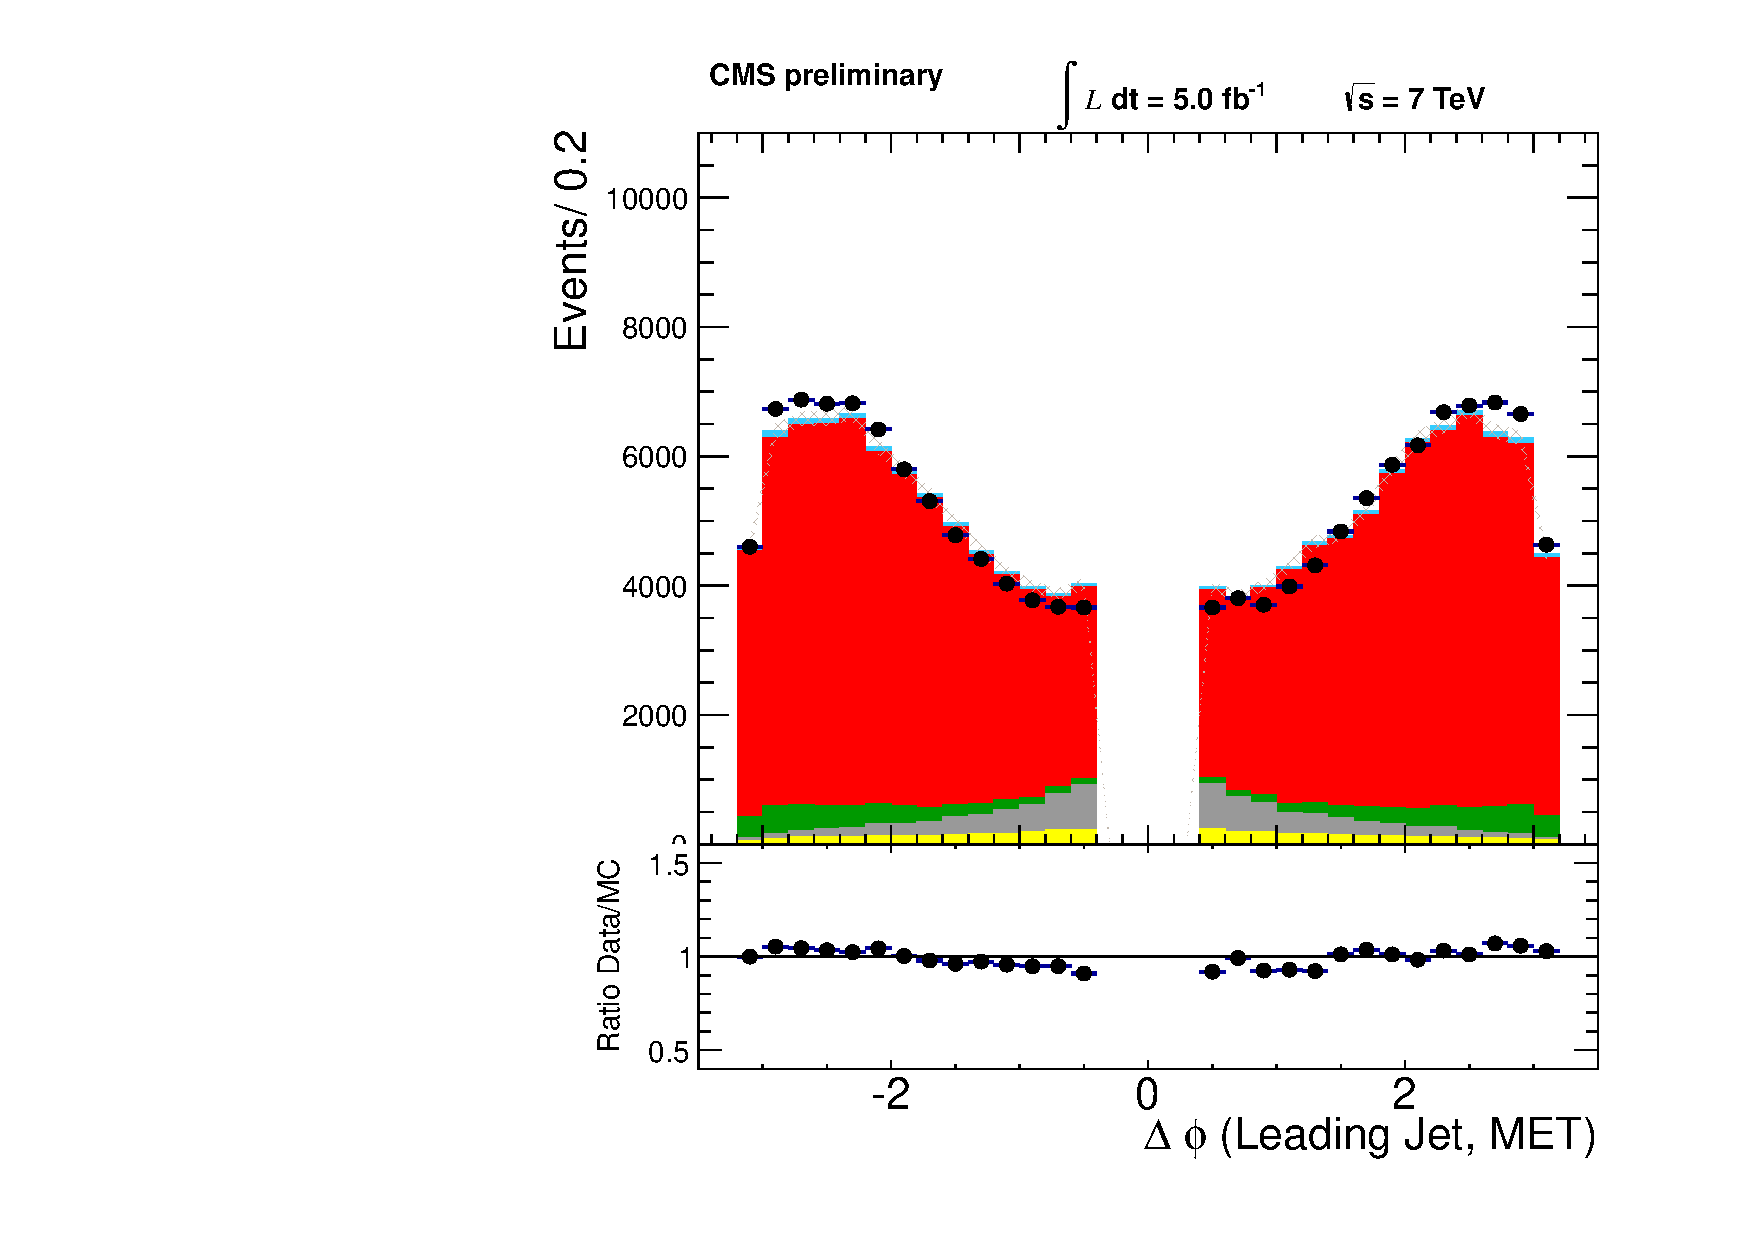
\includegraphics[width=0.49\textwidth]{figs/n-1_plots_el/el_deltaphi_jetldmet.pdf}

    \caption{Comparison of the distributions from data and MC of the
    dijet mass (left) and the $\Delta \phi $ between the leading jet and MET (right)
    for the electron+jets selection.}
    \label{fig:elec_dijetmass}}
\end{figure}
\begin{figure}[h!t]
  {\centering
    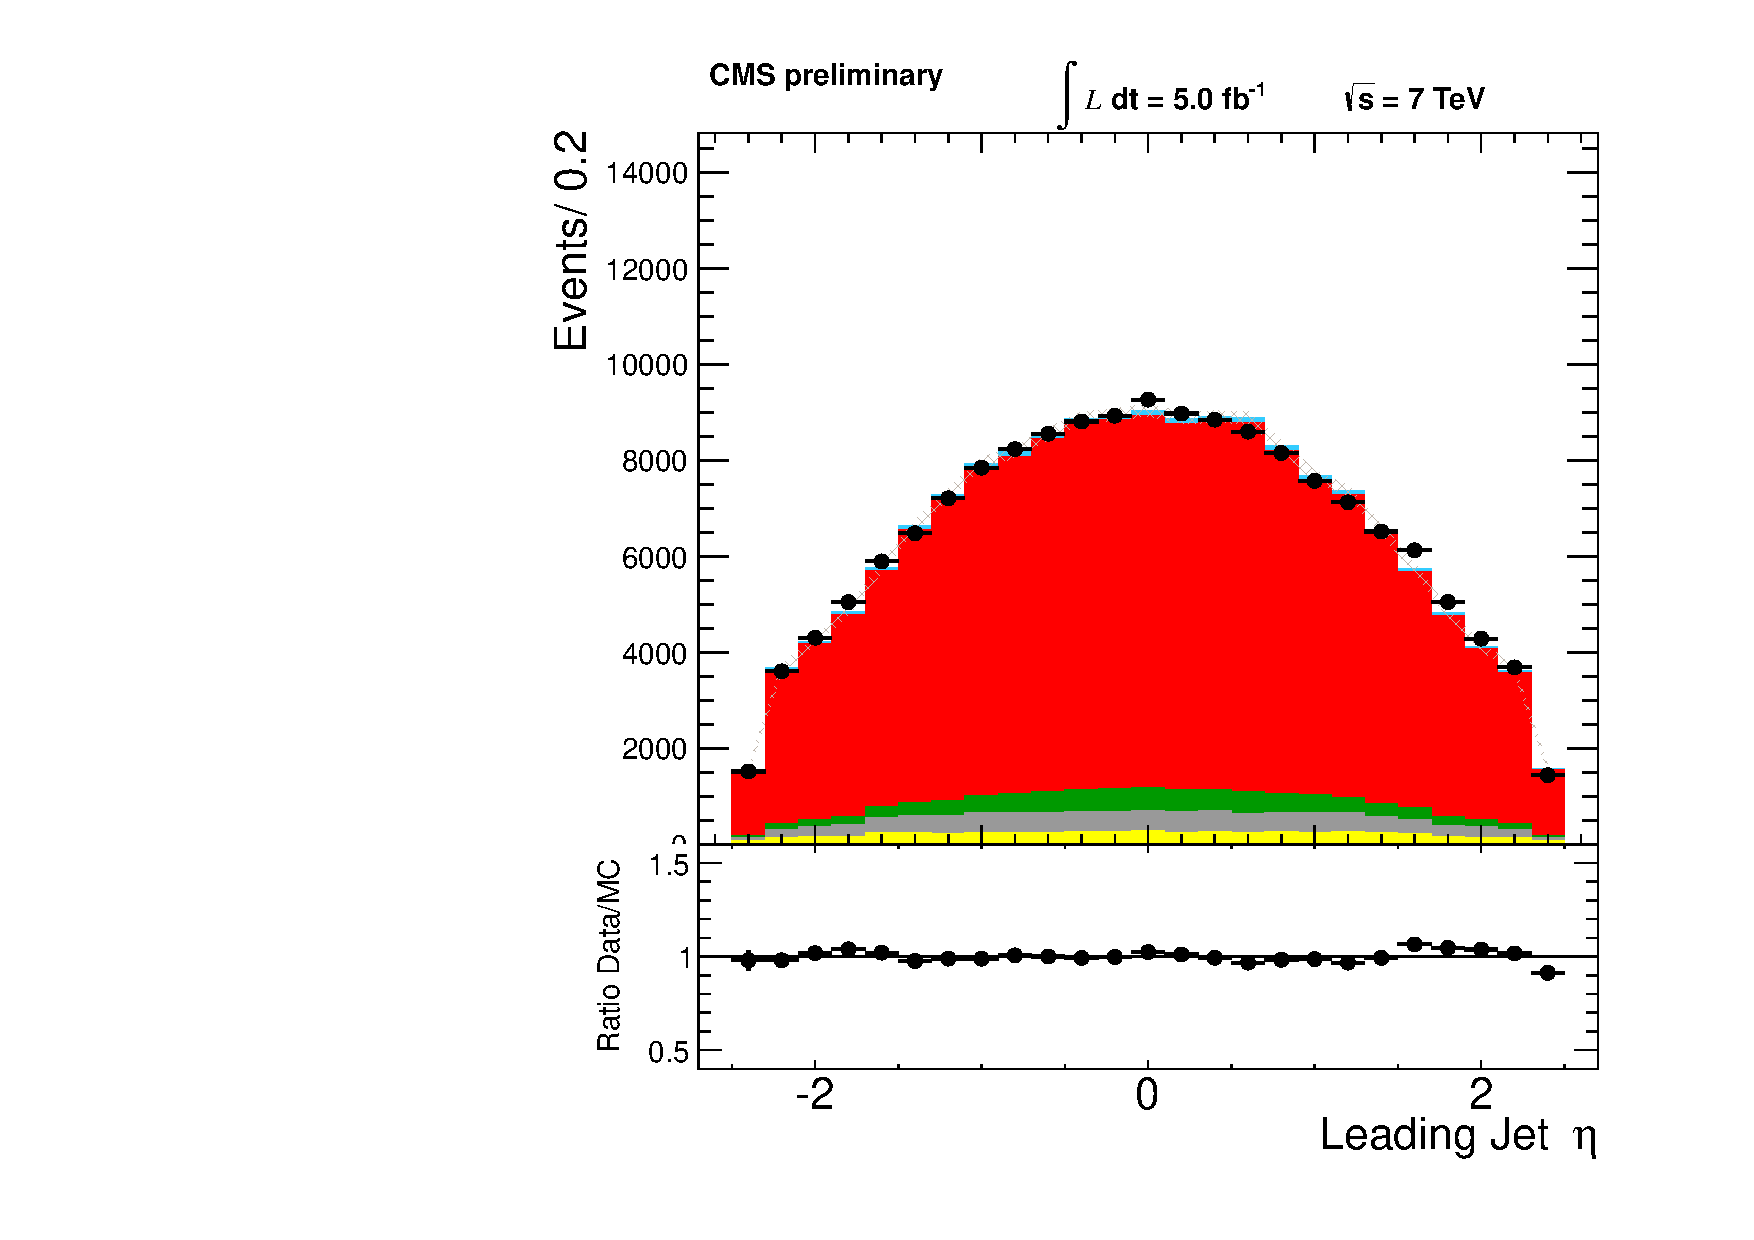
\includegraphics[width=0.49\textwidth]{figs/n-1_plots_el/el_jetld_eta.pdf}
    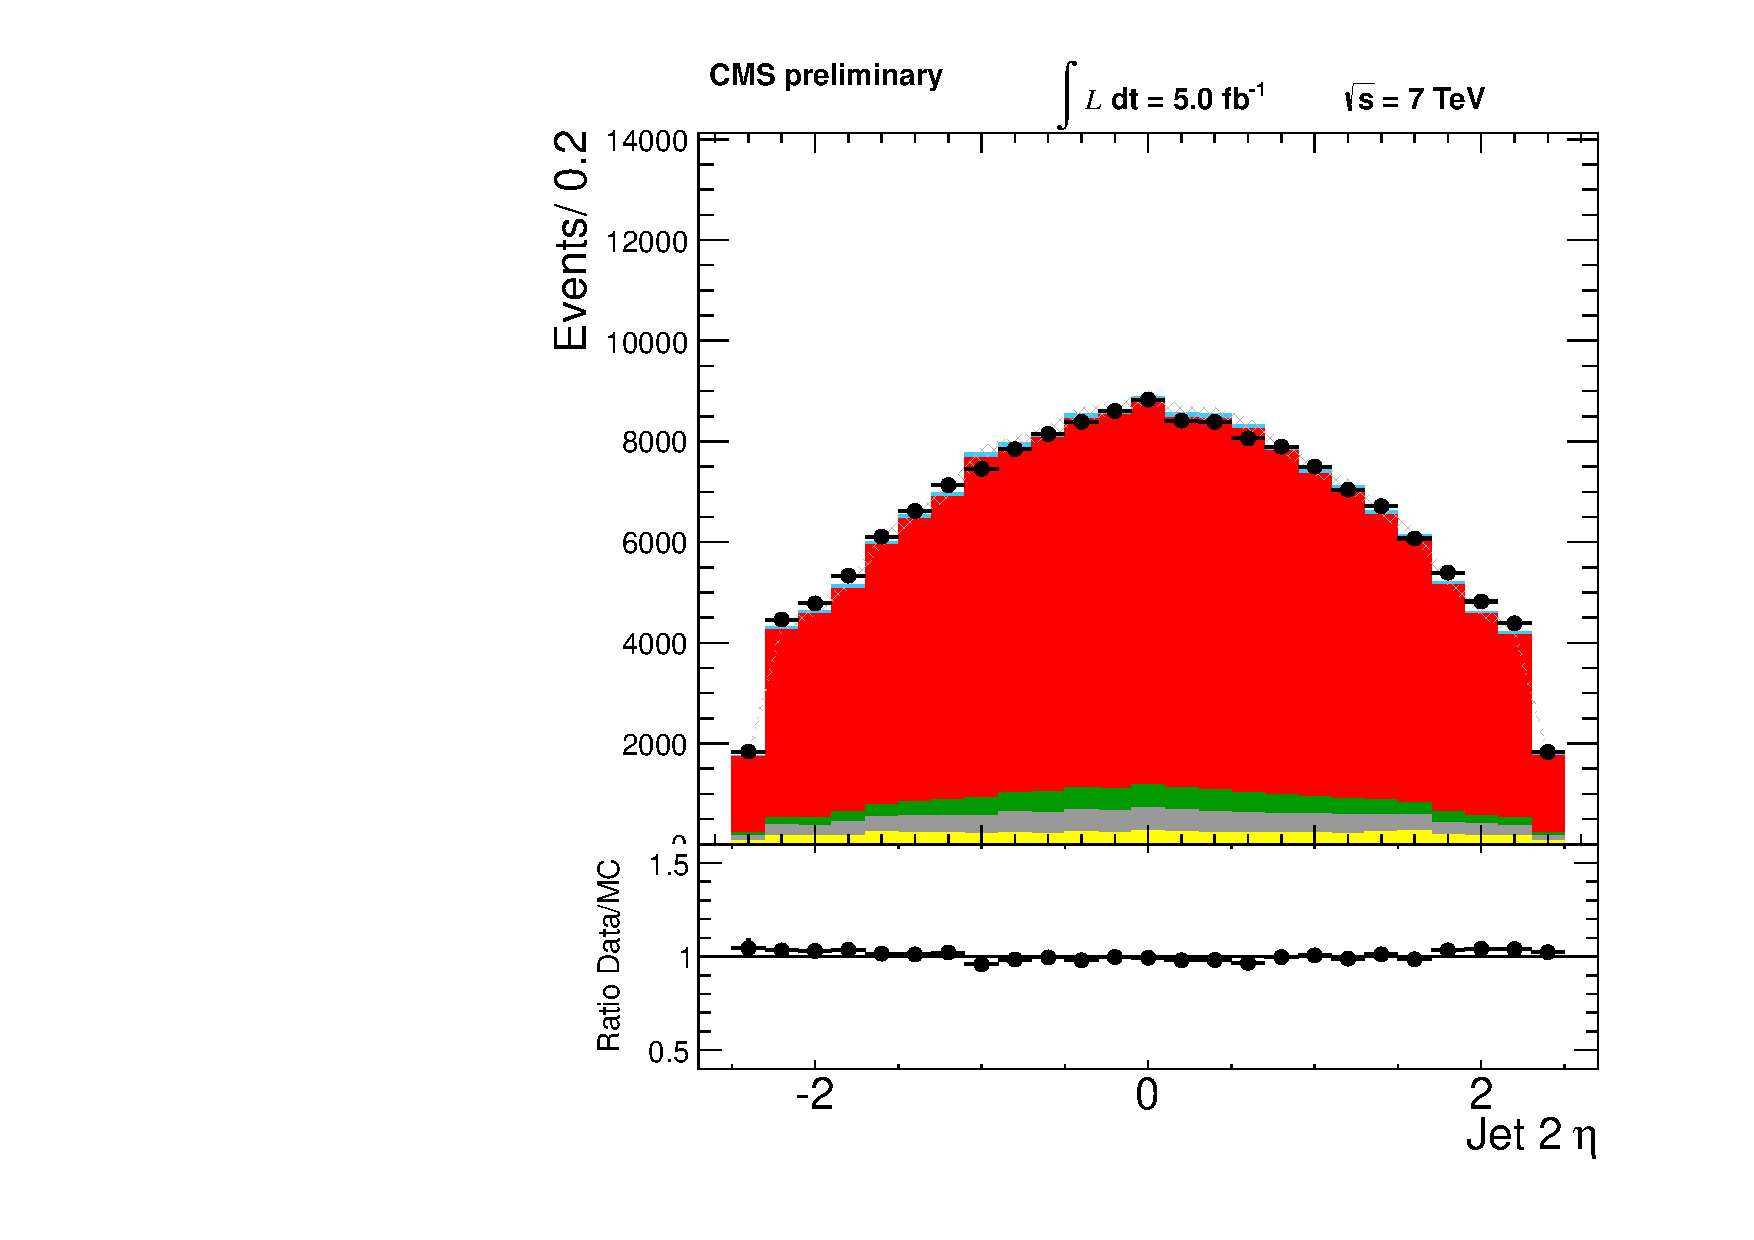
\includegraphics[width=0.49\textwidth]{figs/n-1_plots_el/el_jetnt_eta.pdf}
    \caption{Comparison of the leading jet $\eta $ (left) and the
      second leading jet $\eta $ (right) distributions from data and MC for the electron+jets
      selection. 
      }
    \label{fig:elec_jet_eta}}
\end{figure}
%%%%%%%%%%%%%%%%%%%%%%%%%%%%
\begin{figure}[h!t]
  {\centering
    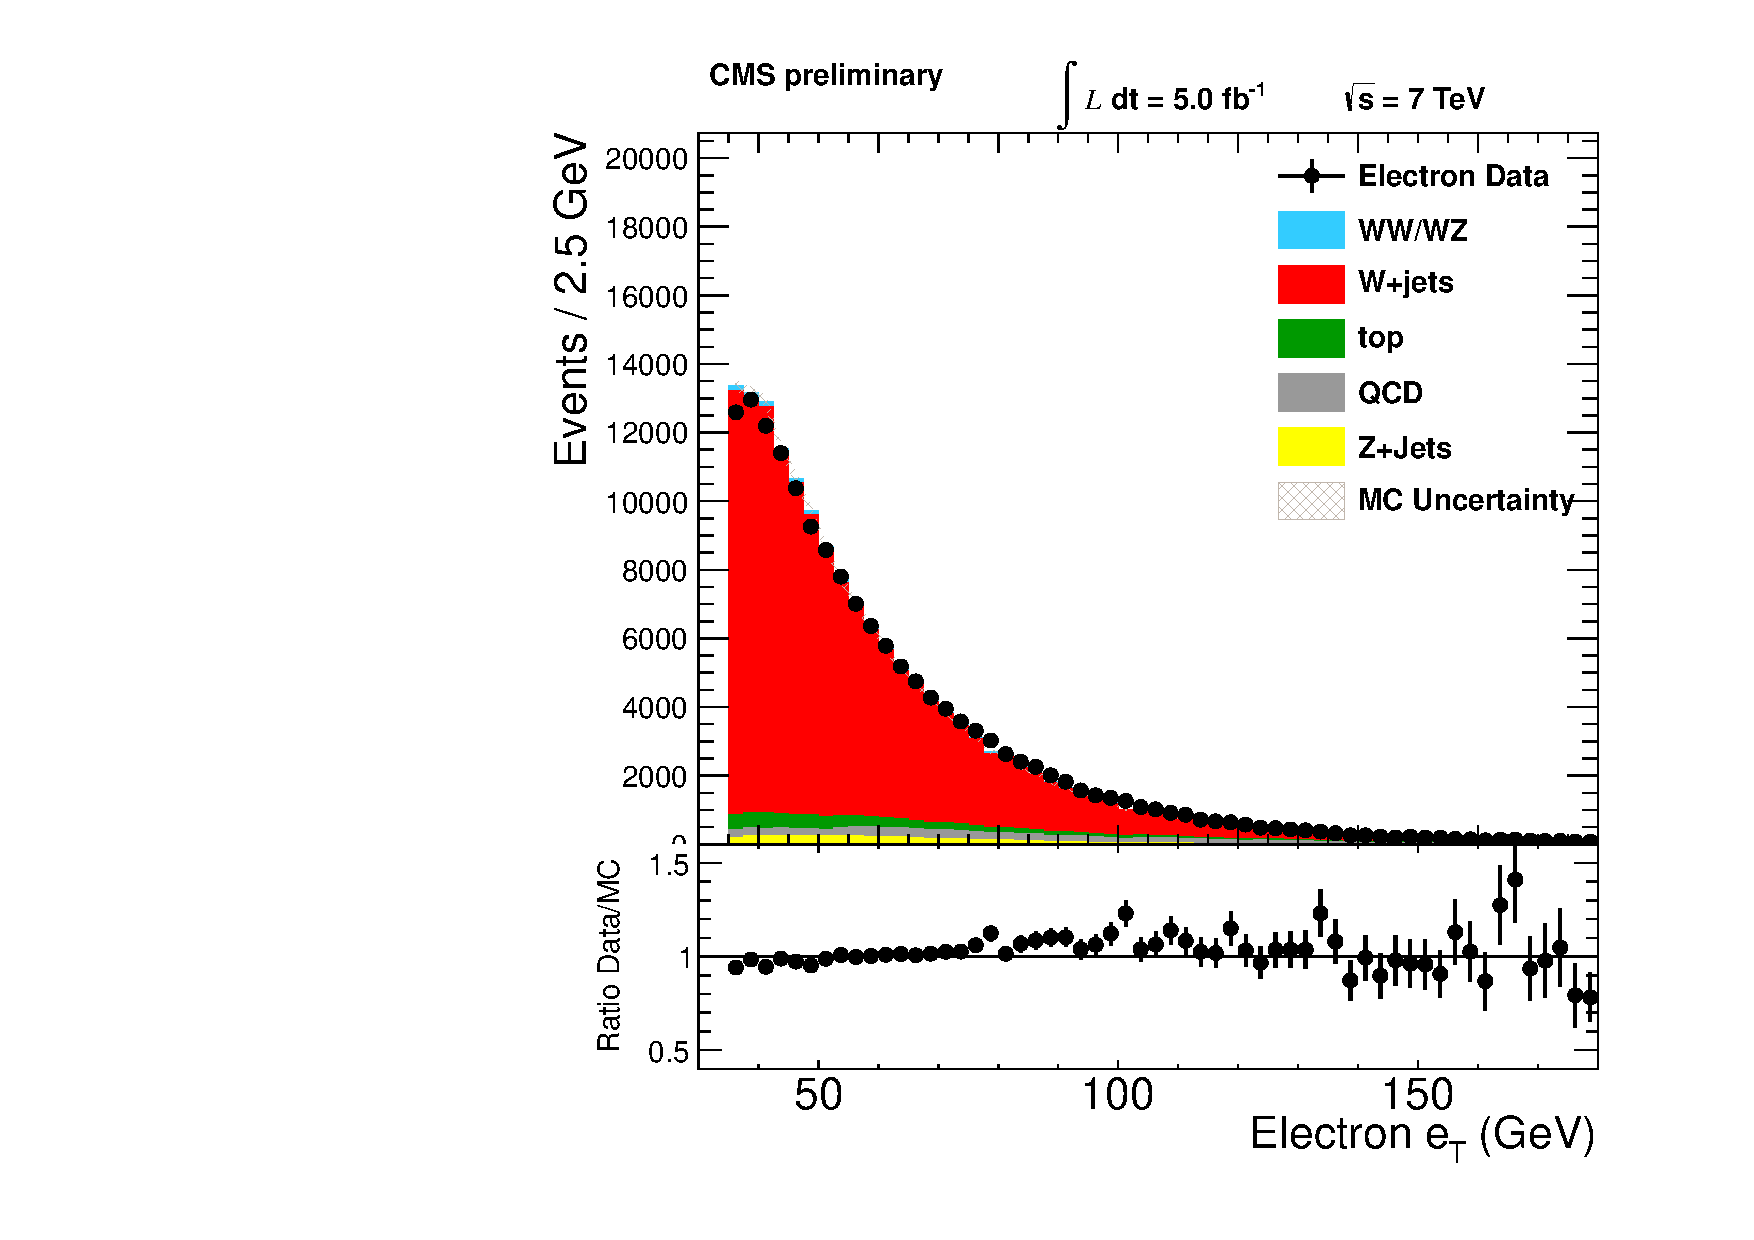
\includegraphics[width=0.49\textwidth]{figs/n-1_plots_el/el_W_electron_et.pdf}
    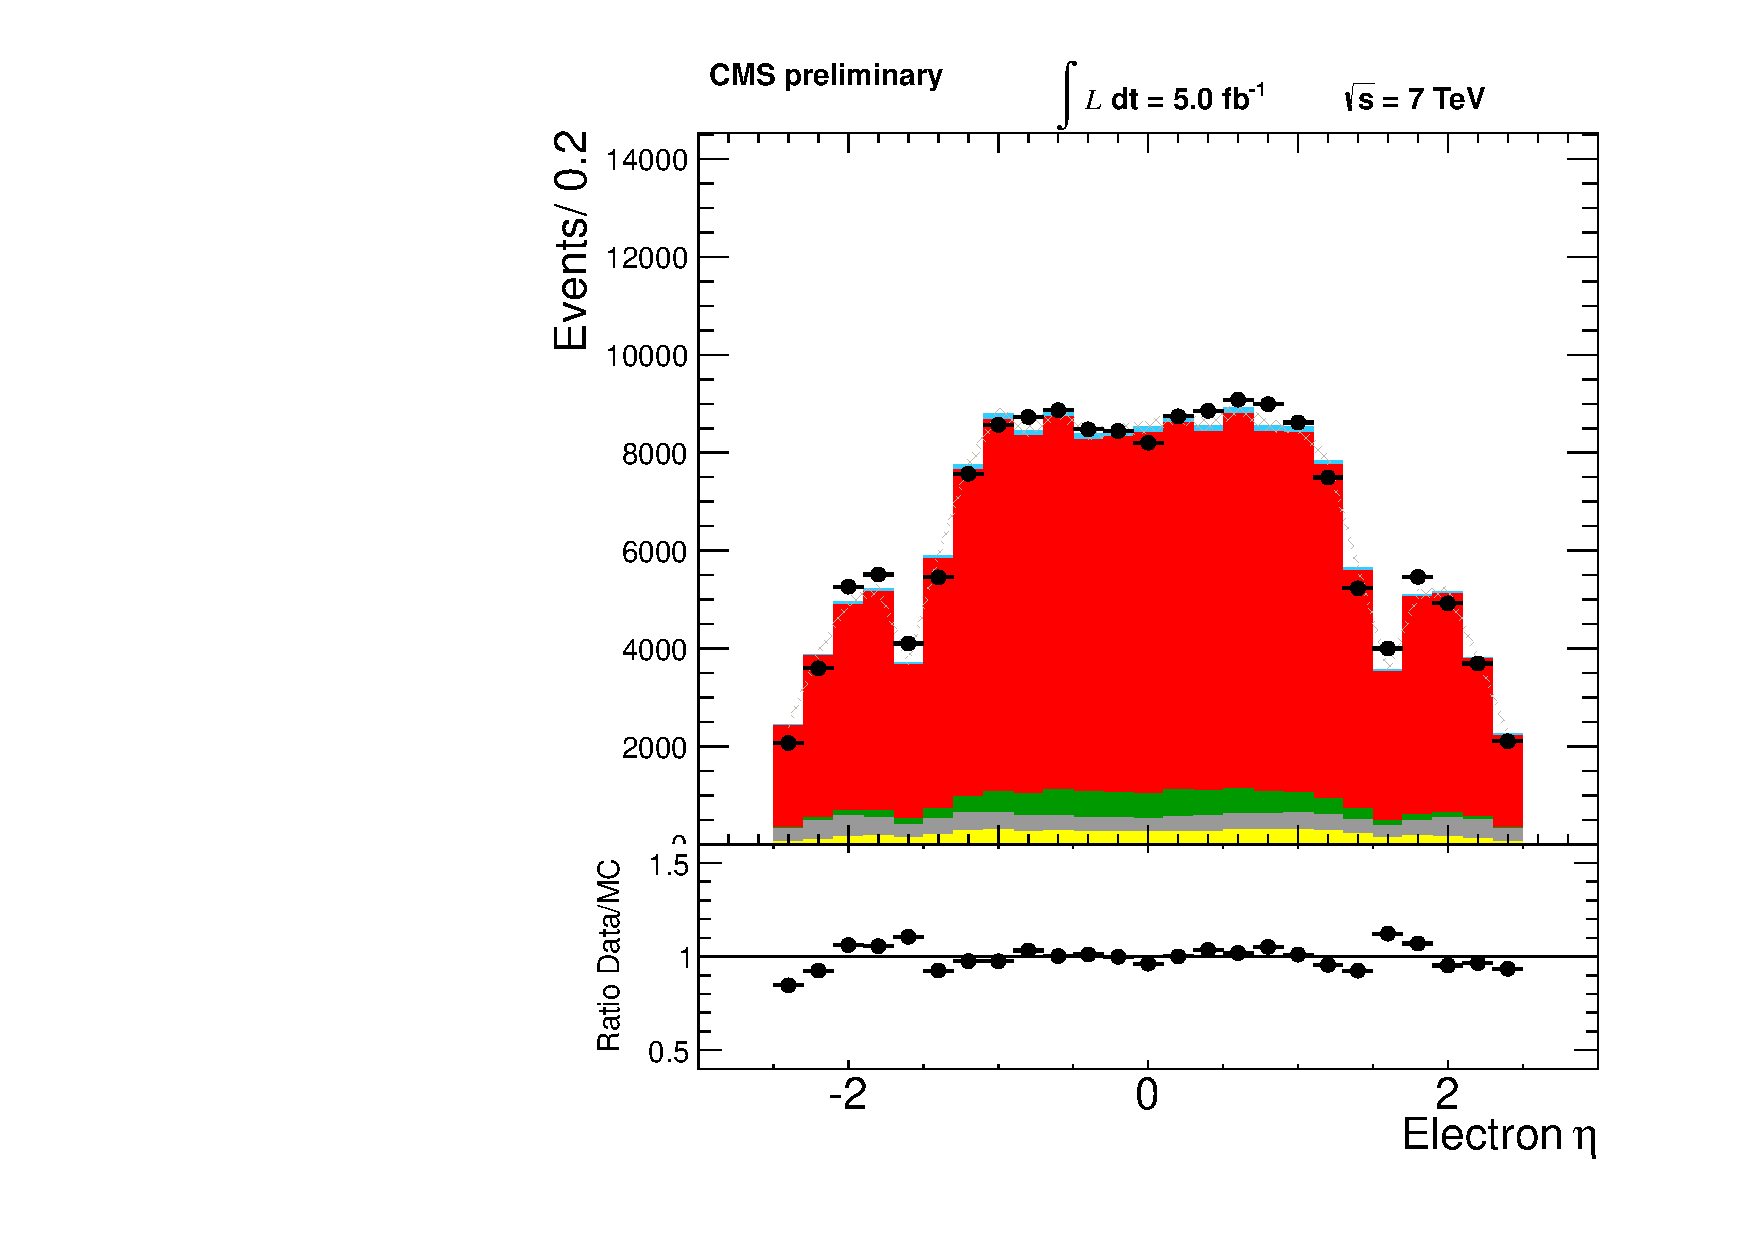
\includegraphics[width=0.49\textwidth]{figs/n-1_plots_el/el_W_electron_eta.pdf}
    \caption{Comparison of the electron $E_{T} $ (left) and the
    electron $\eta $ (right) distributions from data and MC for the
    electron+jets selection. 
    }
   \label{fig:elec_electron}}
\end{figure}
%%%%%%%%%%%%%%%%%%%%%%%%%%%%
\begin{figure}[h!t]
  {\centering
    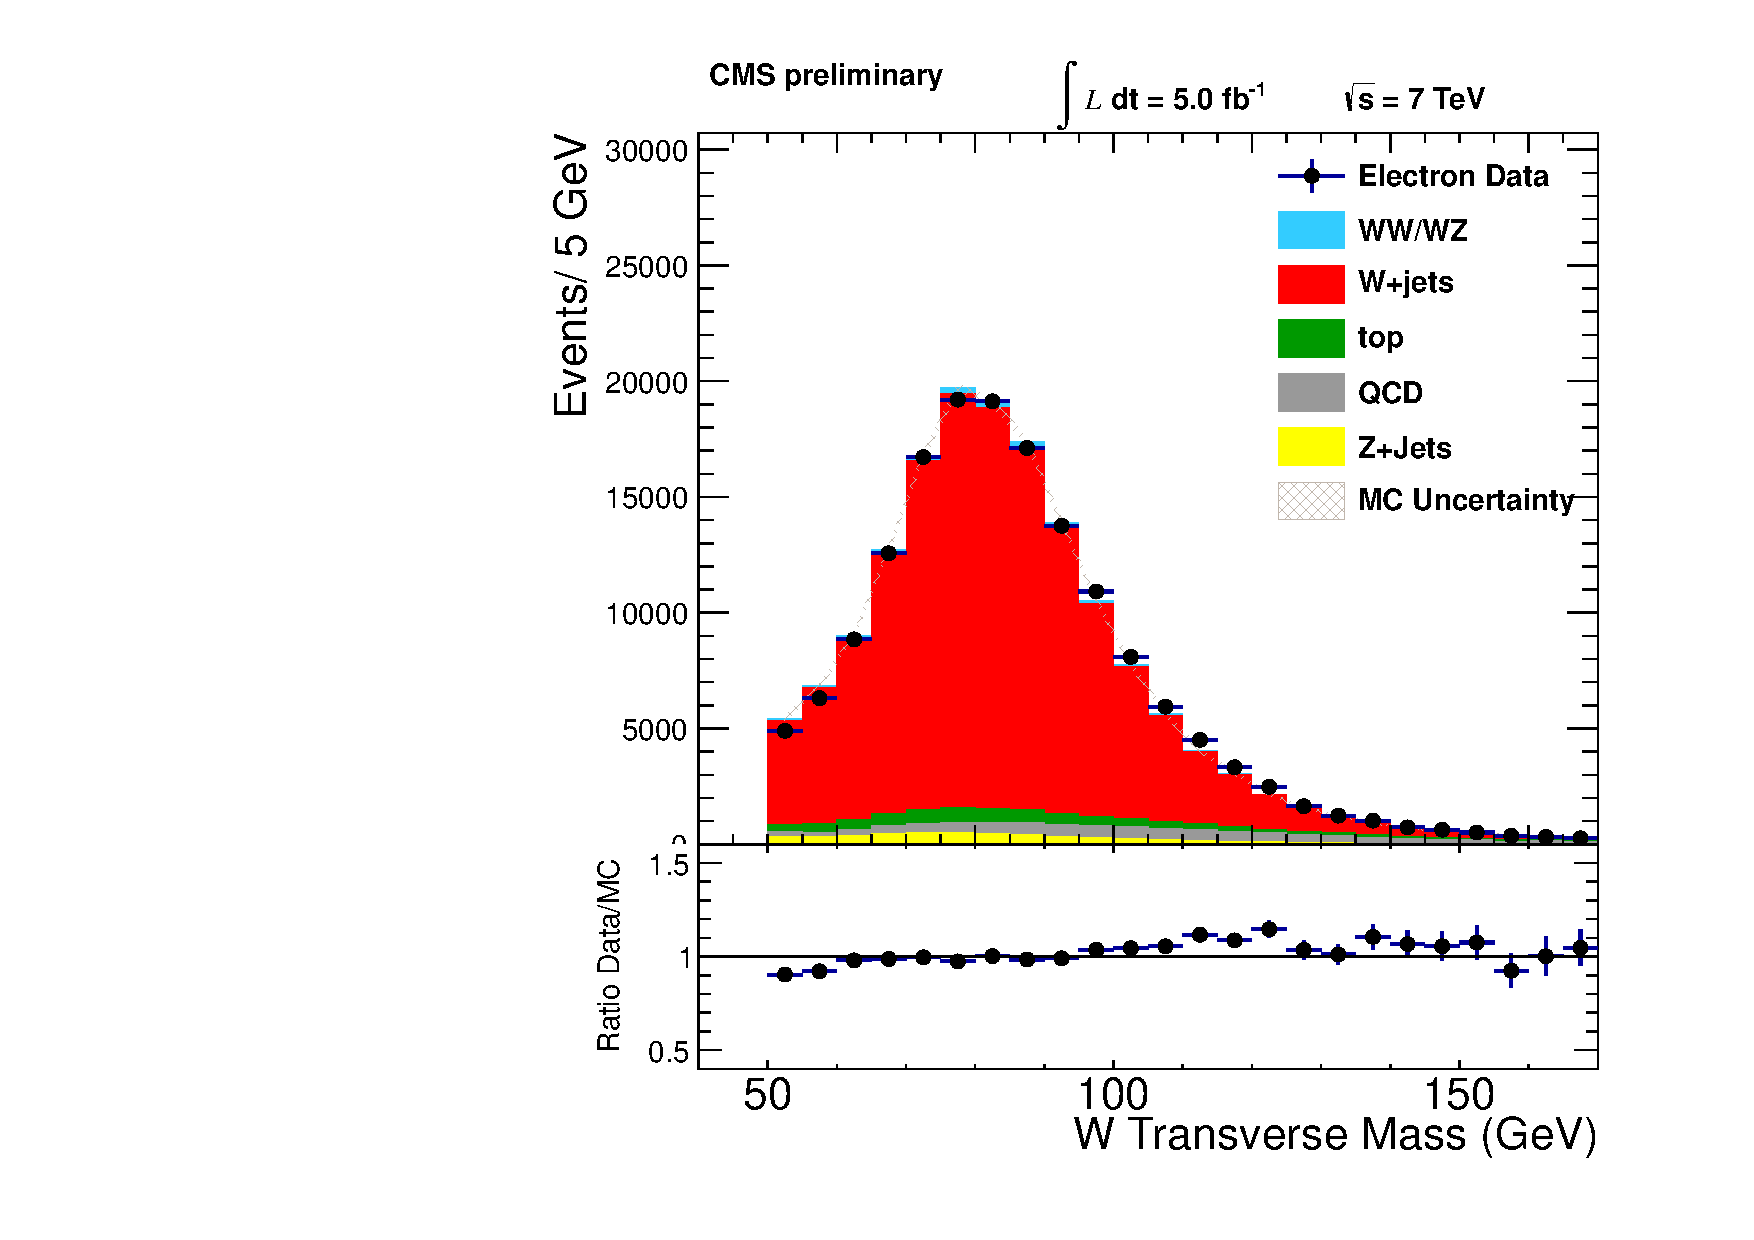
\includegraphics[width=0.49\textwidth]{figs/n-1_plots_el/el_W_mt.pdf}
    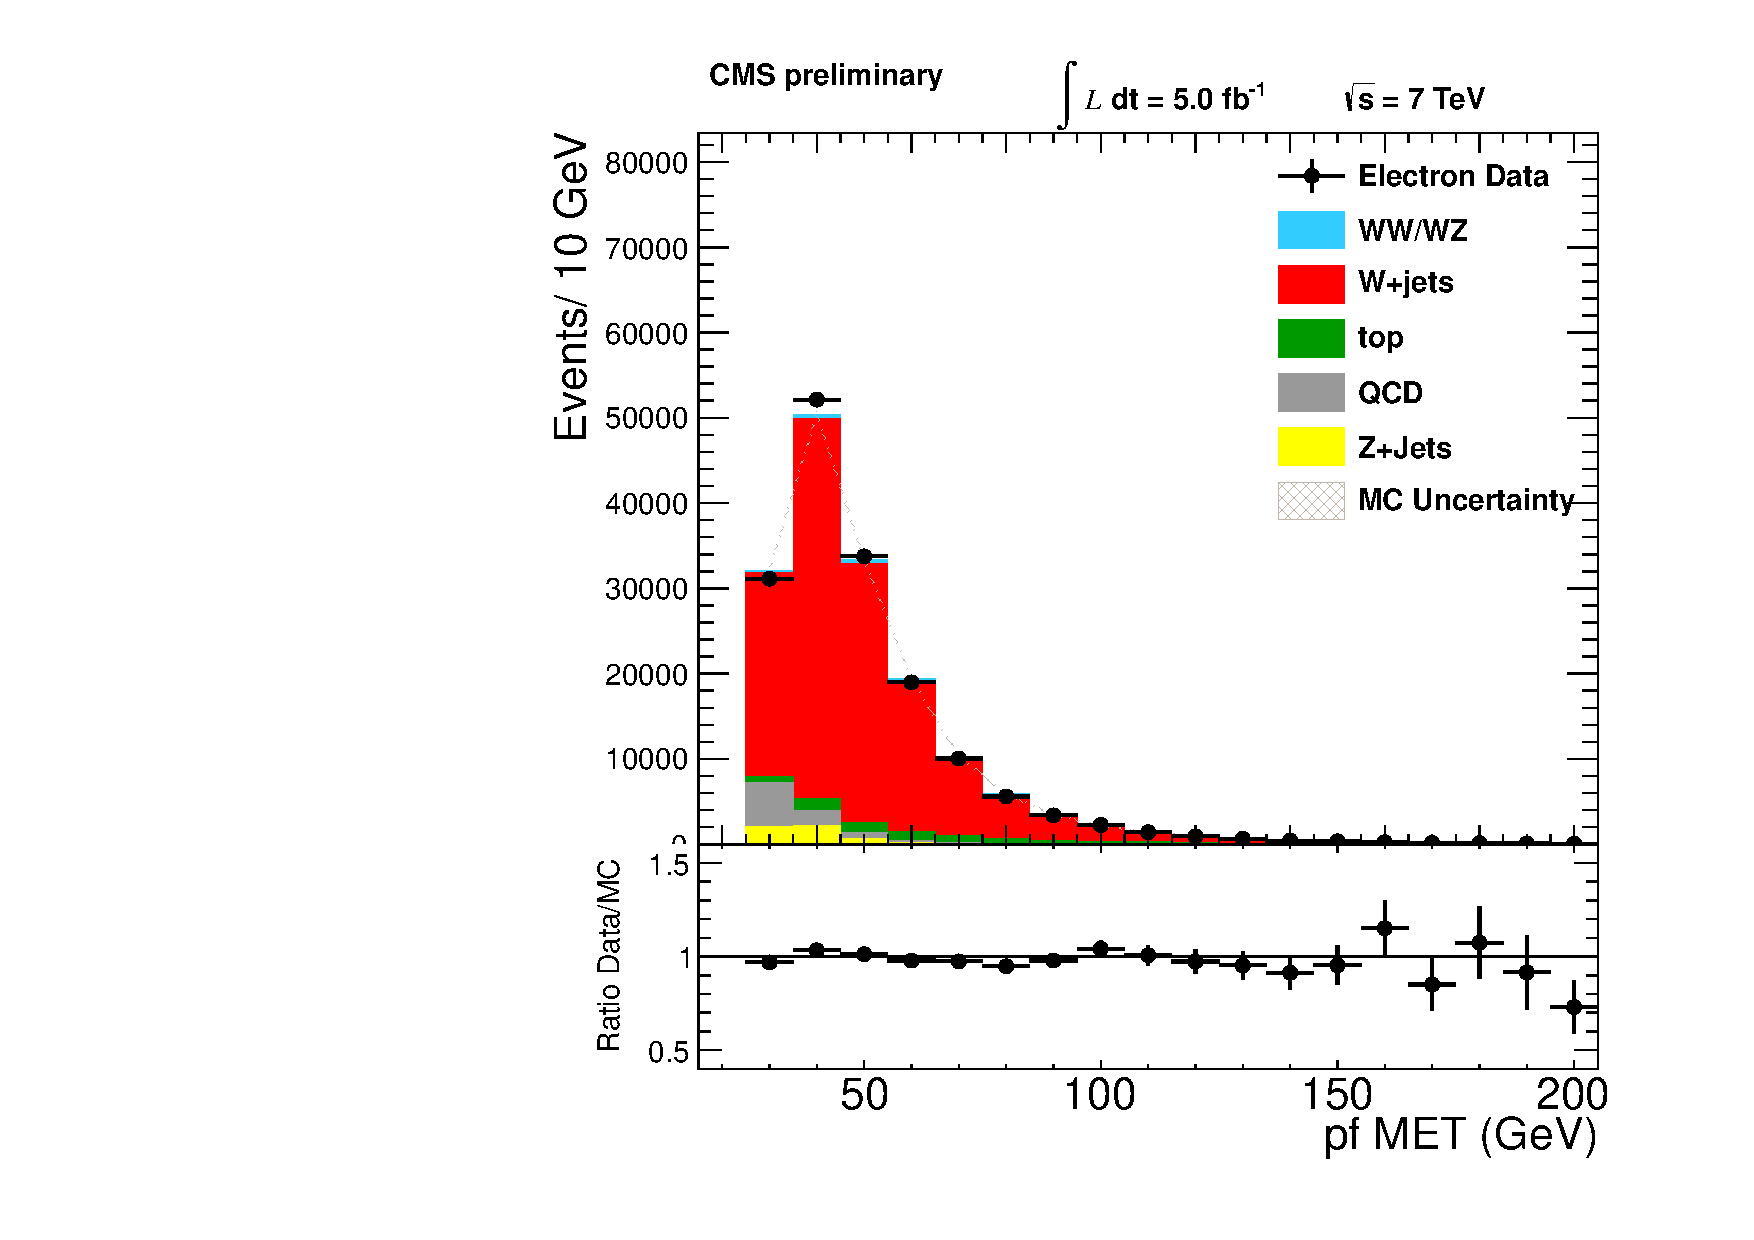
\includegraphics[width=0.49\textwidth]{figs/n-1_plots_el/el_event_met_pfmet.pdf}
    \caption{Comparison of the distributions from data and MC of the transverse mass
     of electron / MET system (left) and the MET (right) for the
      electron+jets selection. 
      }
    \label{fig:elec_W_Mt}}
\end{figure}
%%%%%%%%%%%%%%%%%%%%%%%%%%%%
\begin{figure}[h!t]
  {\centering
    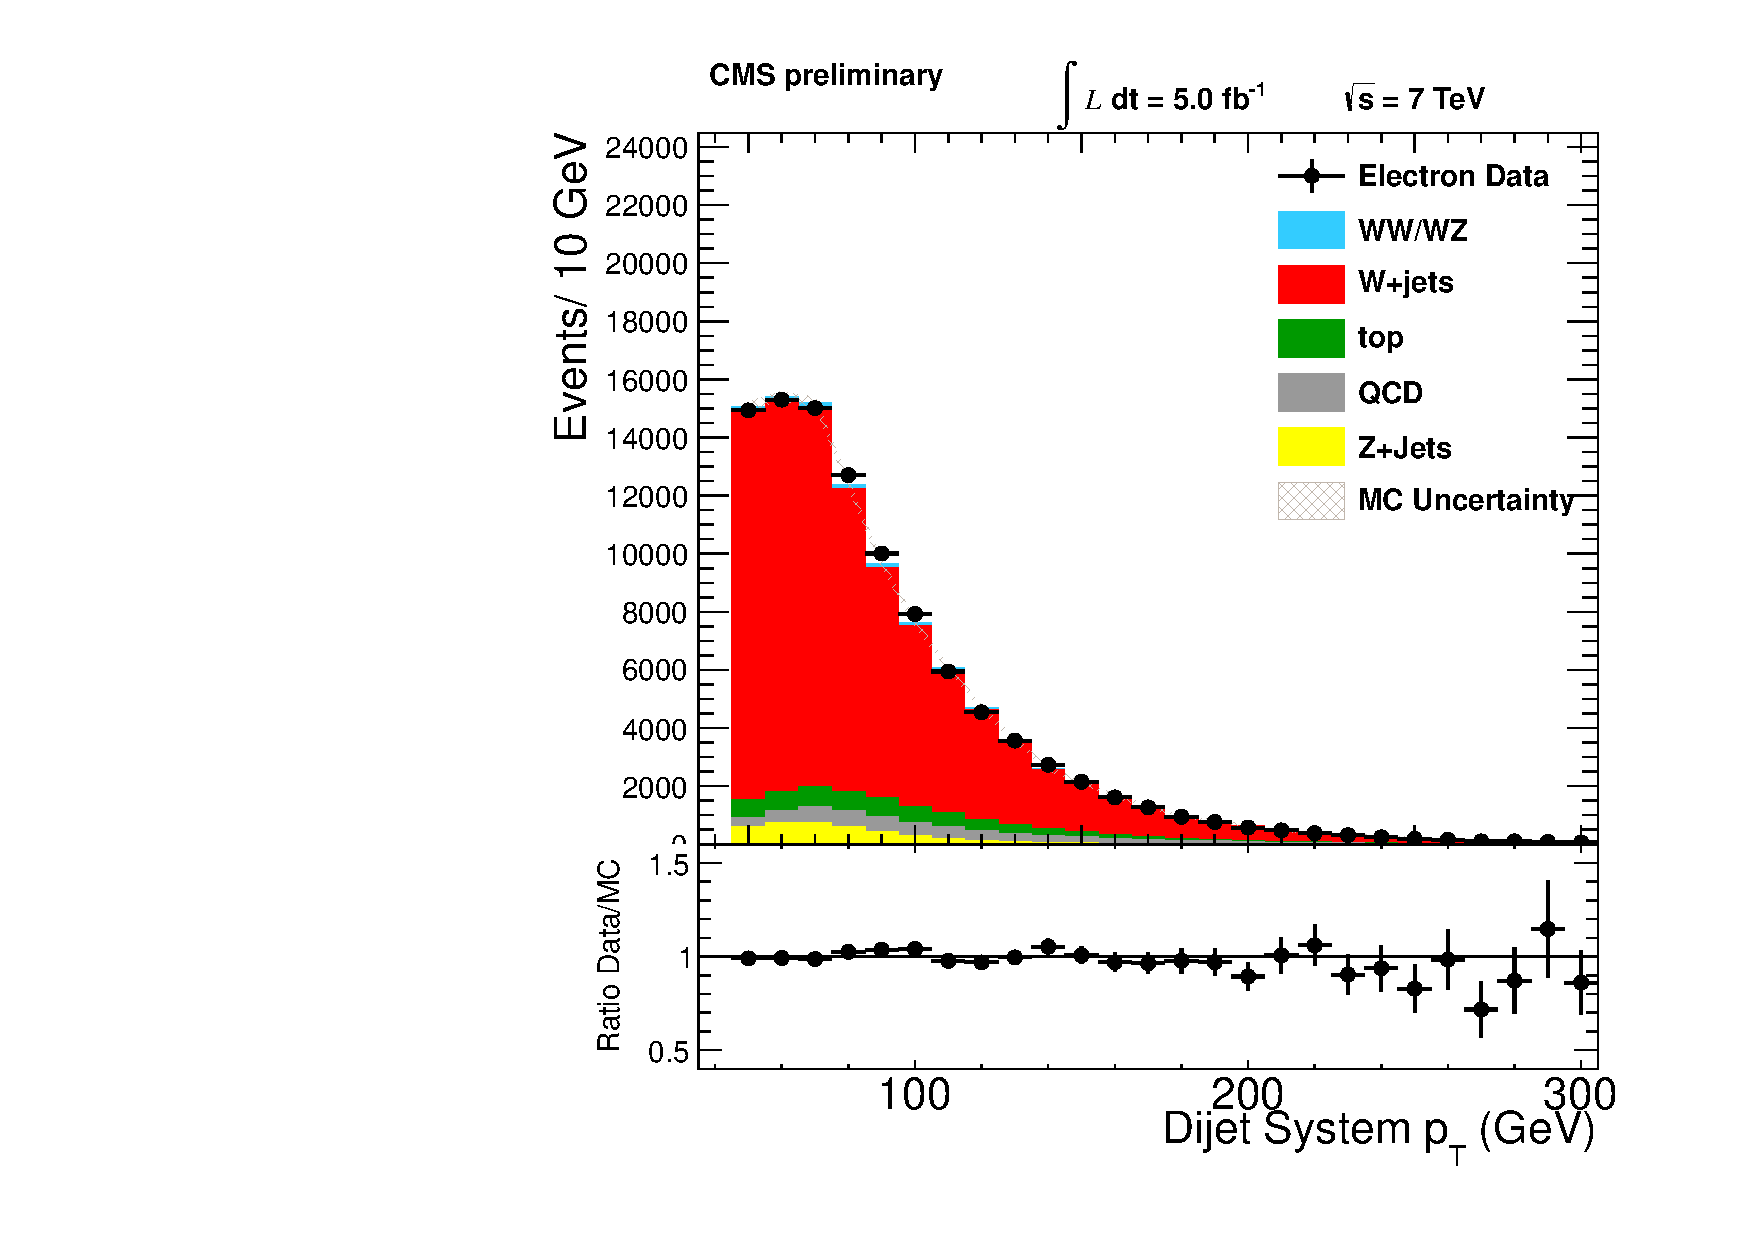
\includegraphics[width=0.49\textwidth]{figs/n-1_plots_el/el_dijet_pt.pdf}
    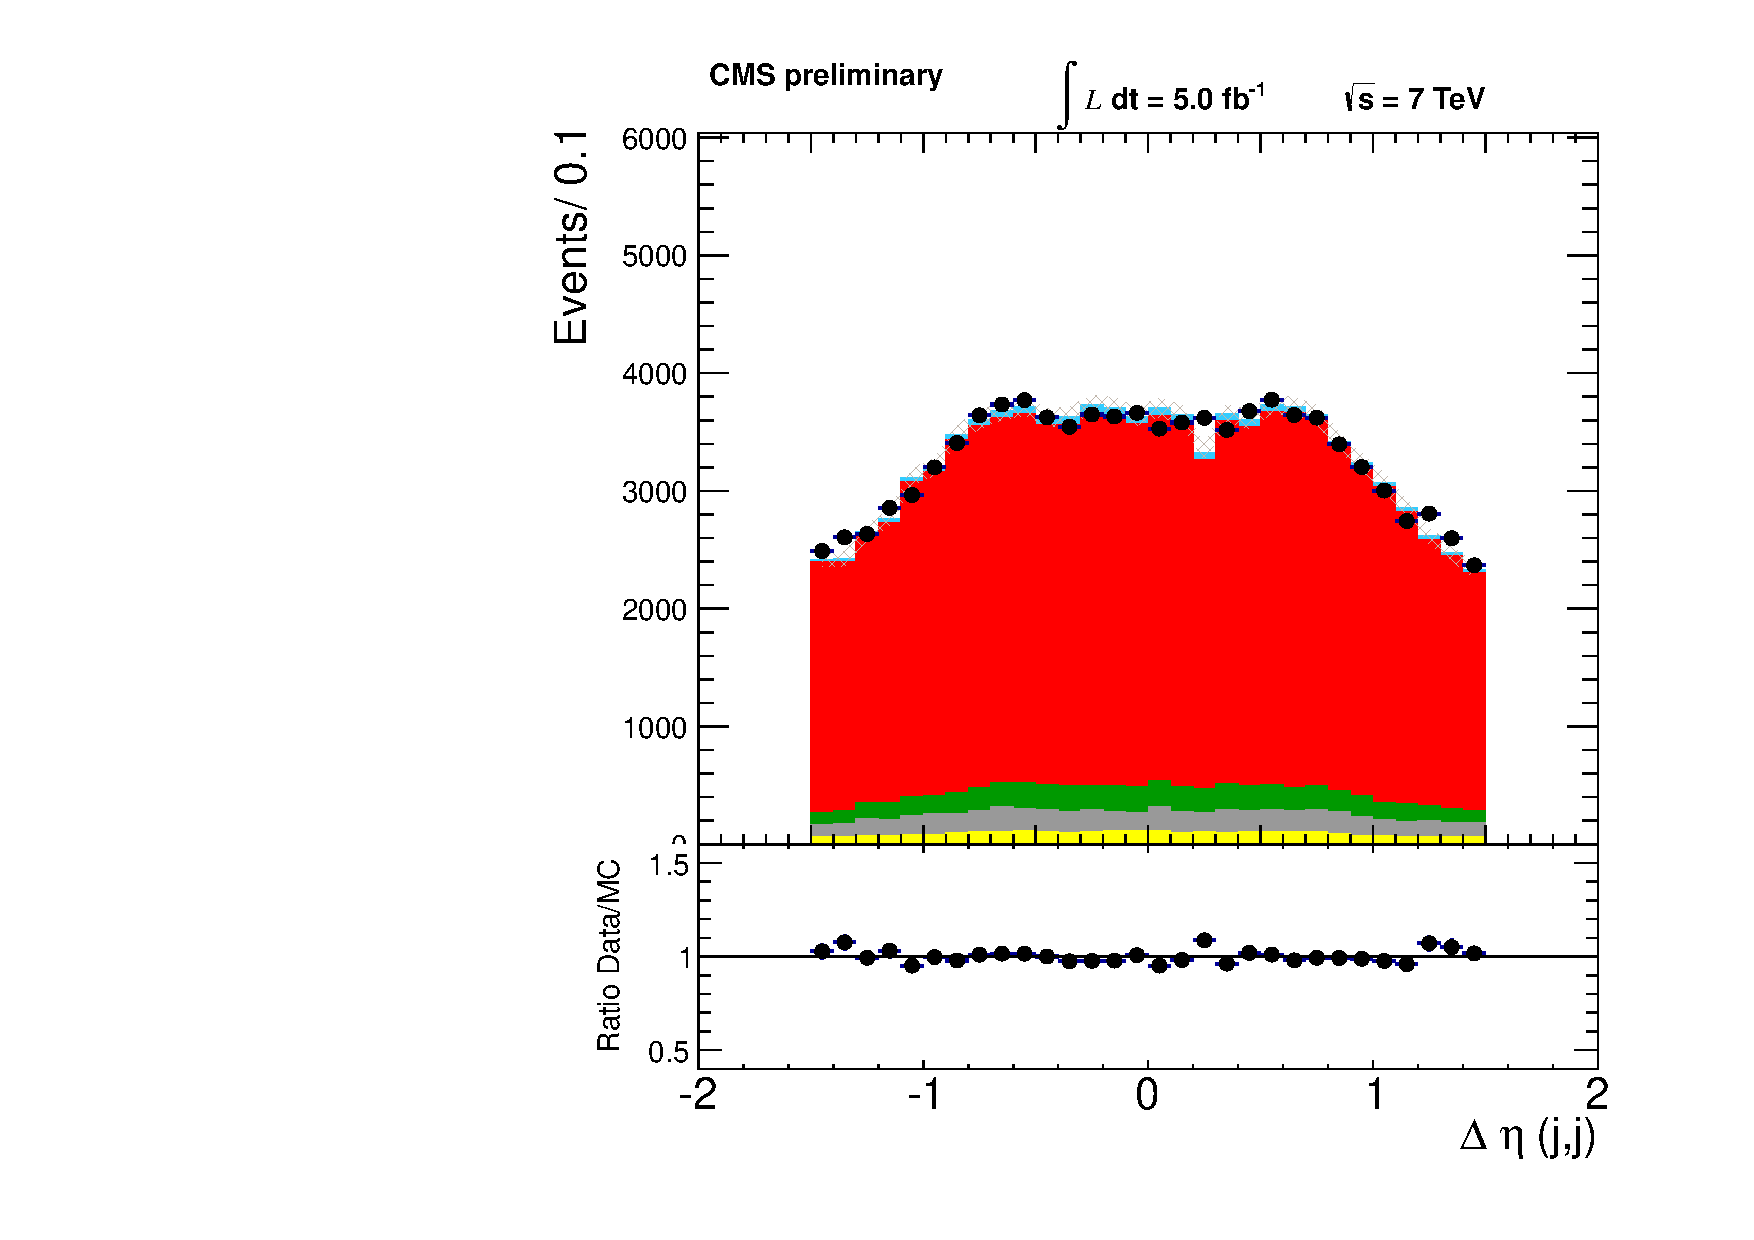
\includegraphics[width=0.49\textwidth]{figs/n-1_plots_el/el_deltaeta_jj.pdf}
    \caption{Comparison of the distributions from data and MC of the dijet system
     $p_{T}$ (left) and the $\eta $ separation between the two jets (right) for the
      electron+jets selection. 
      }
    \label{fig:elec_dijet}}
\end{figure}
%%%%%%%%%%%%%%%%%%%%%%%%%%%%
%%%%%%%%%%%%%%%%%%%%%%%%%%%%
%%%%%%%%%%%%%%%%%%%%%%%%%%%%

\clearpage
%%%%%%%%%%%%%%%%%%%%%%%%%%%%%%%%%%%%%%%%%%%%%%%%%%%%%%%%%%%%%%%%%%%%
%%%%%%%%%%%%%%%%%%%%%%%%%%%%%%%%%%%%%%%%%%%%%%%%%%%%%%%%%%%%%%%%%%%%
%%%%%%%%%%%%%%%%%%%%%%%%%%%%%%%%%%%%%%%%%%%%%%%%%%%%%%%%%%%%%%%%%%%%
\section{Lepton reconstruction/selection efficiencies}
\label{sec:lepeff}
Lepton reconstruction and selection efficiencies are computed using
a ``Tag \& Probe'' technique on the Drell-Yan Z$\to\ell\ell$ events in
both data and MC~\cite{tagnprobe}.  The ratios of data versus MC efficiencies for
various steps of lepton reconstruction/selection are given below. If such
a ratio is found to be statistically inconsistent with unity, it is
applied as a scale factor correction to the MC samples.
%%%%%%%%%%%%%%%%%%
\subsection{Muon reconstruction/isolation corrections}
%%%%%%%%%%%
The efficiency scale factor for muon isolation is given in
Table~\ref{tab:muonEffsRecoToIso_ScaleFactors}.  The scale factor is
statistically consistent with unity throughout.  Results consistent
with these were also obtained by the Drell-Yan group using
Z$\rightarrow\mu\mu$ events.
Figure~\ref{fig:muonisoeffsf} shows this scale factor variation in $m_{jj}$.
%\verbatiminput{muonEffsRecoToIso_ScaleFactors.txt}
%%%%%%%%%%%%%%%%%%%%%%%%%%%%%
\begin{table}[bthp]
\begin{center}
  \begin{tabular}{l l c | l c}
    \hline  \hline
    $p_T$ range (GeV) & $\eta$ range  &
    $\frac{\epsilon_{\rm{Data}}}{\epsilon_{\rm{MC}}}$ & 
    $\eta$ range  & $\frac{\epsilon_{\rm{Data}}}{\epsilon_{\rm{MC}}}$\\
    \hline  
    25--30 &	-2.1-- -1.5 &	1.00  & 1.5--2.1   & 1.00 \\
           &	-1.5-- -1.0 &	0.99  & 1.0--1.5   & 1.00 \\
           &	-1.0-- -0.5 &	1.00  & 0.5--1.0   & 1.00 \\
           &	-0.5--	0.0 &	1.00  & 0.0--0.5   & 1.00 \\
    \hline  
    30--35 &	-2.1-- -1.5 &	1.00  & 1.5--2.1   & 1.00 \\
           &	-1.5-- -1.0 &	0.99  & 1.0--1.5   & 1.00 \\
           &	-1.0-- -0.5 &	1.00  & 0.5--1.0   & 1.00 \\
           &	-0.5--	0.0 &	1.00  & 0.0--0.5   & 1.00 \\
    \hline  
    35--40 &	-2.1-- -1.5 &	0.99  & 1.5--2.1   & 1.00 \\
           &	-1.5-- -1.0 &	0.99  & 1.0--1.5   & 1.00 \\
           &	-1.0-- -0.5 &	1.00  & 0.5--1.0   & 1.00 \\
           &	-0.5--	0.0 &	1.00  & 0.0--0.5   & 1.00 \\
    \hline  
    40--45 &	-2.1-- -1.5 &	1.00  & 1.5--2.1   & 1.00 \\
           &	-1.5-- -1.0 &	0.99  & 1.0--1.5   & 1.00 \\
           &	-1.0-- -0.5 &	1.00  & 0.5--1.0   & 1.00 \\
           &	-0.5--	0.0 &	1.00  & 0.0--0.5   & 1.00 \\
    \hline  
    45--50 &	-2.1-- -1.5 &	1.00  & 1.5--2.1   & 1.00 \\
           &	-1.5-- -1.0 &	0.99  & 1.0--1.5   & 1.00 \\
           &	-1.0-- -0.5 &	1.00  & 0.5--1.0   & 1.00 \\
           &	-0.5--	0.0 &	1.00  & 0.0--0.5   & 1.00 \\
    \hline  
    50--200&	-2.1-- -1.5 &	1.00  & 1.5--2.1   & 1.00 \\
           &	-1.5-- -1.0 &	0.99  & 1.0--1.5   & 1.00 \\
           &	-1.0-- -0.5 &	1.00  & 0.5--1.0   & 1.00 \\
           &	-0.5--	0.0 &	1.00  & 0.0--0.5   & 1.00 \\
    \hline  \hline
  \end{tabular}
\end{center}
\caption{\label{tab:muonEffsRecoToIso_ScaleFactors}
Muon isolation efficiency data/MC scale factors. The statistical uncertainties were found
to be negligible, while the systematic uncertainty is $\sim$2\%. There is a 
$\sim$1\% difference in muon isolation efficiency in barrel between data and MC.}
\end{table}
%%%%%%%%%%%%
\subsection{Electron reconstruction scale factors}
The efficiency scale factor for electron reconstruction is given in 
Table~\ref{tab:eleEffsSCToReco_ScaleFactors}.
The scale factor is statistically consistent with unity throughout.
Figure~\ref{fig:electronRecoIDeffsf} shows this scale factor variation in $m_{jj}$.
%%%%%%%%%%%
%\verbatiminput{eleEffsSCToReco_ScaleFactors.txt}
%%%%%%%%%%%%%%%%%%%%%%%%%%%%%
\begin{table}[bthp]
\begin{center}
  \begin{tabular}{l l c | l c}
    \hline  \hline
    $p_T$ range (GeV) & $\eta$ range  &
    $\frac{\epsilon_{\rm{Data}}}{\epsilon_{\rm{MC}}}$ & 
    $\eta$ range  & $\frac{\epsilon_{\rm{Data}}}{\epsilon_{\rm{MC}}}$\\
    \hline  
    30--35 &	-2.5-- -1.5 & 1.0096 $\pm$ 0.0062 & 1.5--2.5 & 1.0094 $\pm$ 0.0015 \\
           &	-1.5-- 0.0  & 1.0060 $\pm$ 0.0029 & 0.0--1.5 & 1.0021 $\pm$ 0.0029 \\
    \hline  
    35--40 &	-2.5-- -1.5 & 1.0038 $\pm$ 0.0043 & 1.5--2.5 & 1.0135 $\pm$ 0.0040 \\
           &	-1.5-- 0.0  & 0.9987 $\pm$ 0.0016 & 0.0--1.5 & 0.9935 $\pm$ 0.0016 \\
    \hline  
    40--45 &	-2.5-- -1.5 & 1.0002 $\pm$ 0.0070 & 1.5--2.5 & 1.0111 $\pm$ 0.0034 \\
           &	-1.5-- 0.0  & 0.9951 $\pm$ 0.0012 & 0.0--1.5 & 0.9941 $\pm$ 0.0012 \\
    \hline  
    45--50 &	-2.5-- -1.5 & 1.0202 $\pm$ 0.0021 & 1.5--2.5 & 1.0170 $\pm$ 0.0080 \\
           &	-1.5-- 0.0  & 0.9941 $\pm$ 0.0014 & 0.0--1.5 & 0.9967 $\pm$ 0.0013 \\
    \hline  
    50--200&	-2.5-- -1.5 & 1.0287 $\pm$ 0.0049 & 1.5--2.5 & 1.0421 $\pm$ 0.0092 \\
           &	-1.5-- 0.0  & 0.9805 $\pm$ 0.0130 & 0.0--1.5 & 0.9989 $\pm$ 0.0018 \\
    \hline  \hline
  \end{tabular}
\end{center}
\caption{\label{tab:eleEffsSCToReco_ScaleFactors}
Electron reconstruction efficiency data/MC scale factors. The uncertainties are statistical only.}
\end{table}
%%%%%%%%%%%%%%%%%%%%%%%%%%%%%
%%%%%%%%%%%%%%%%%%%%
\begin{figure}[h!t]
  {\centering
  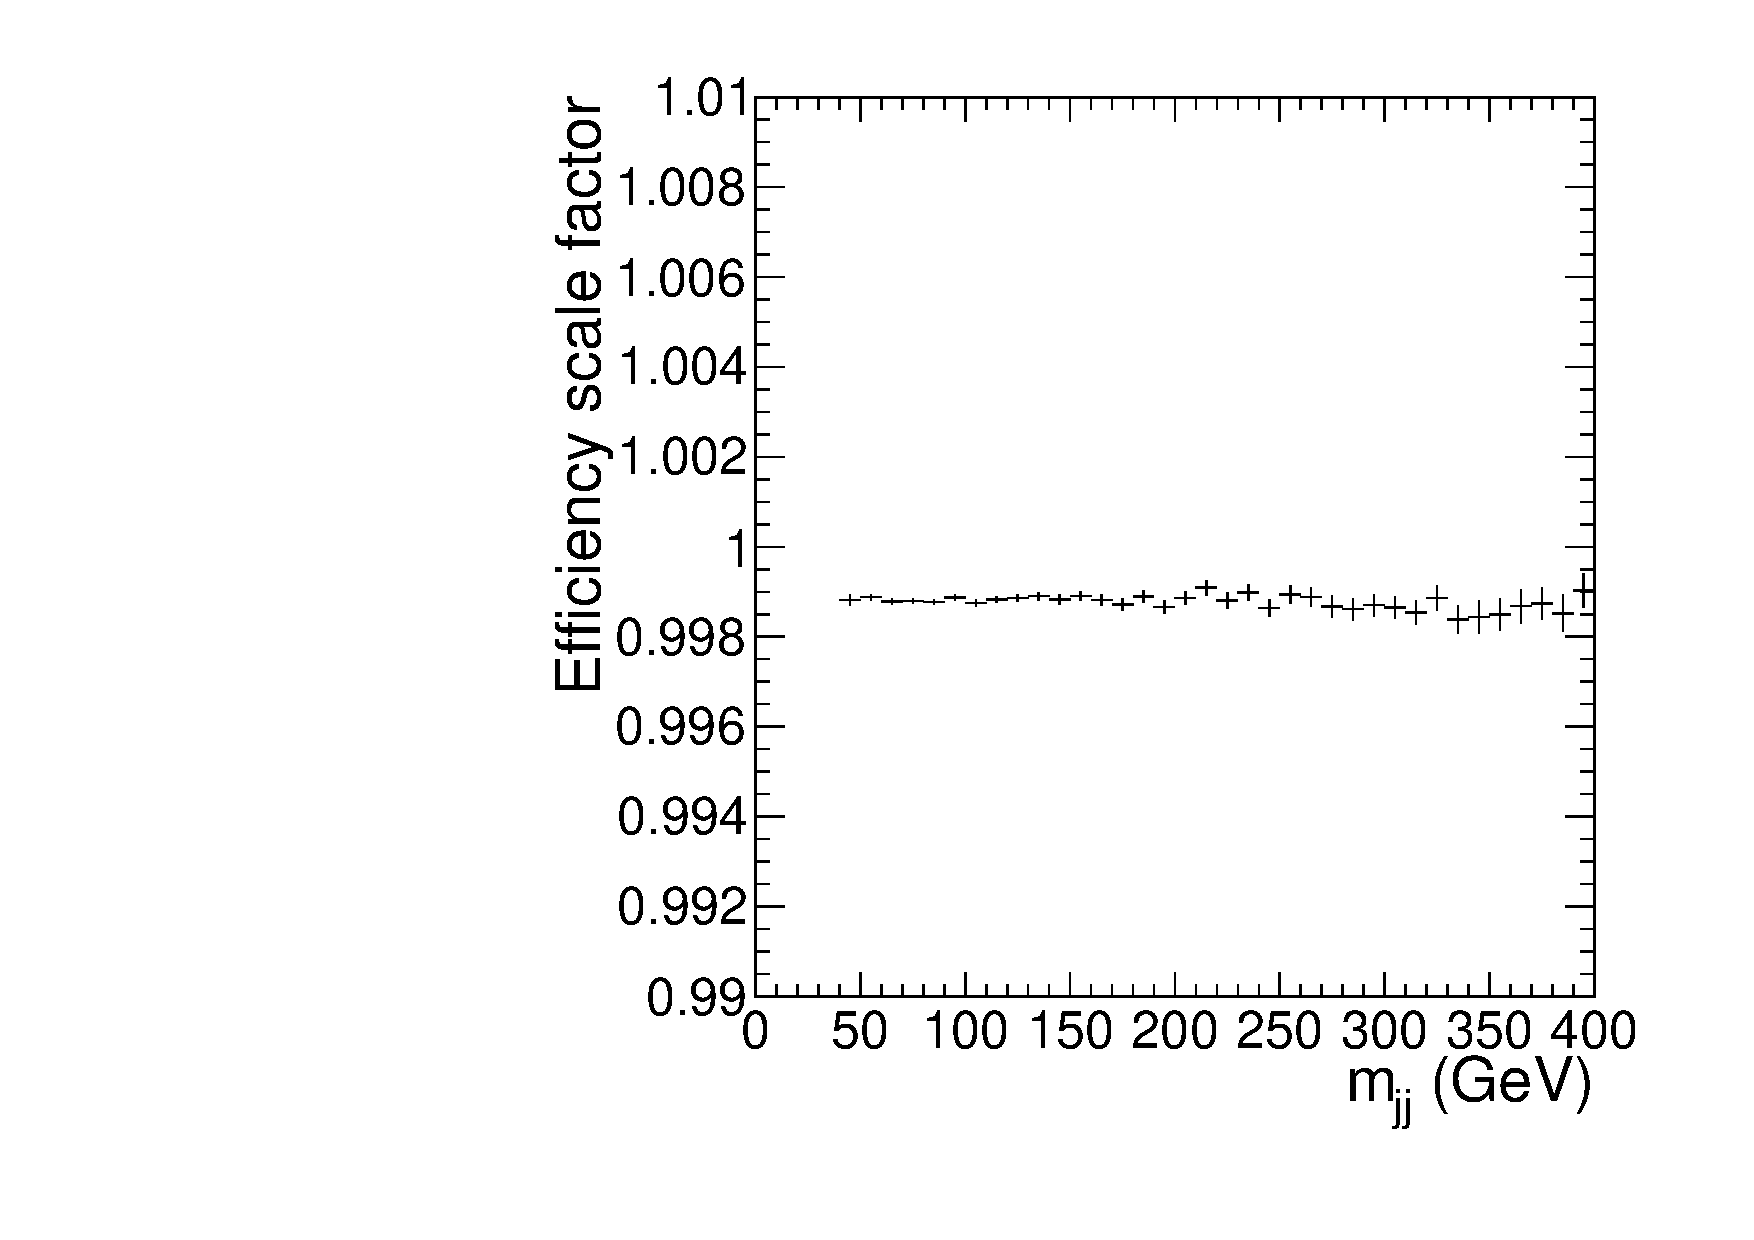
\includegraphics[width=0.48\textwidth]{figs/effPlots/fig_eff_mu_RecoToIso_ScaleFactors.pdf}
   \caption{Luminosity weighted average efficiency scale factors (data/MC) for muon isolation.}
\label{fig:muonisoeffsf}}
\end{figure}
%%%%%%%%%%%%%%%%%%%%
%%%%%%%%%%%%%%%%%%%%
\begin{figure}[h!t]
  {\centering
  \subfigure[]{
  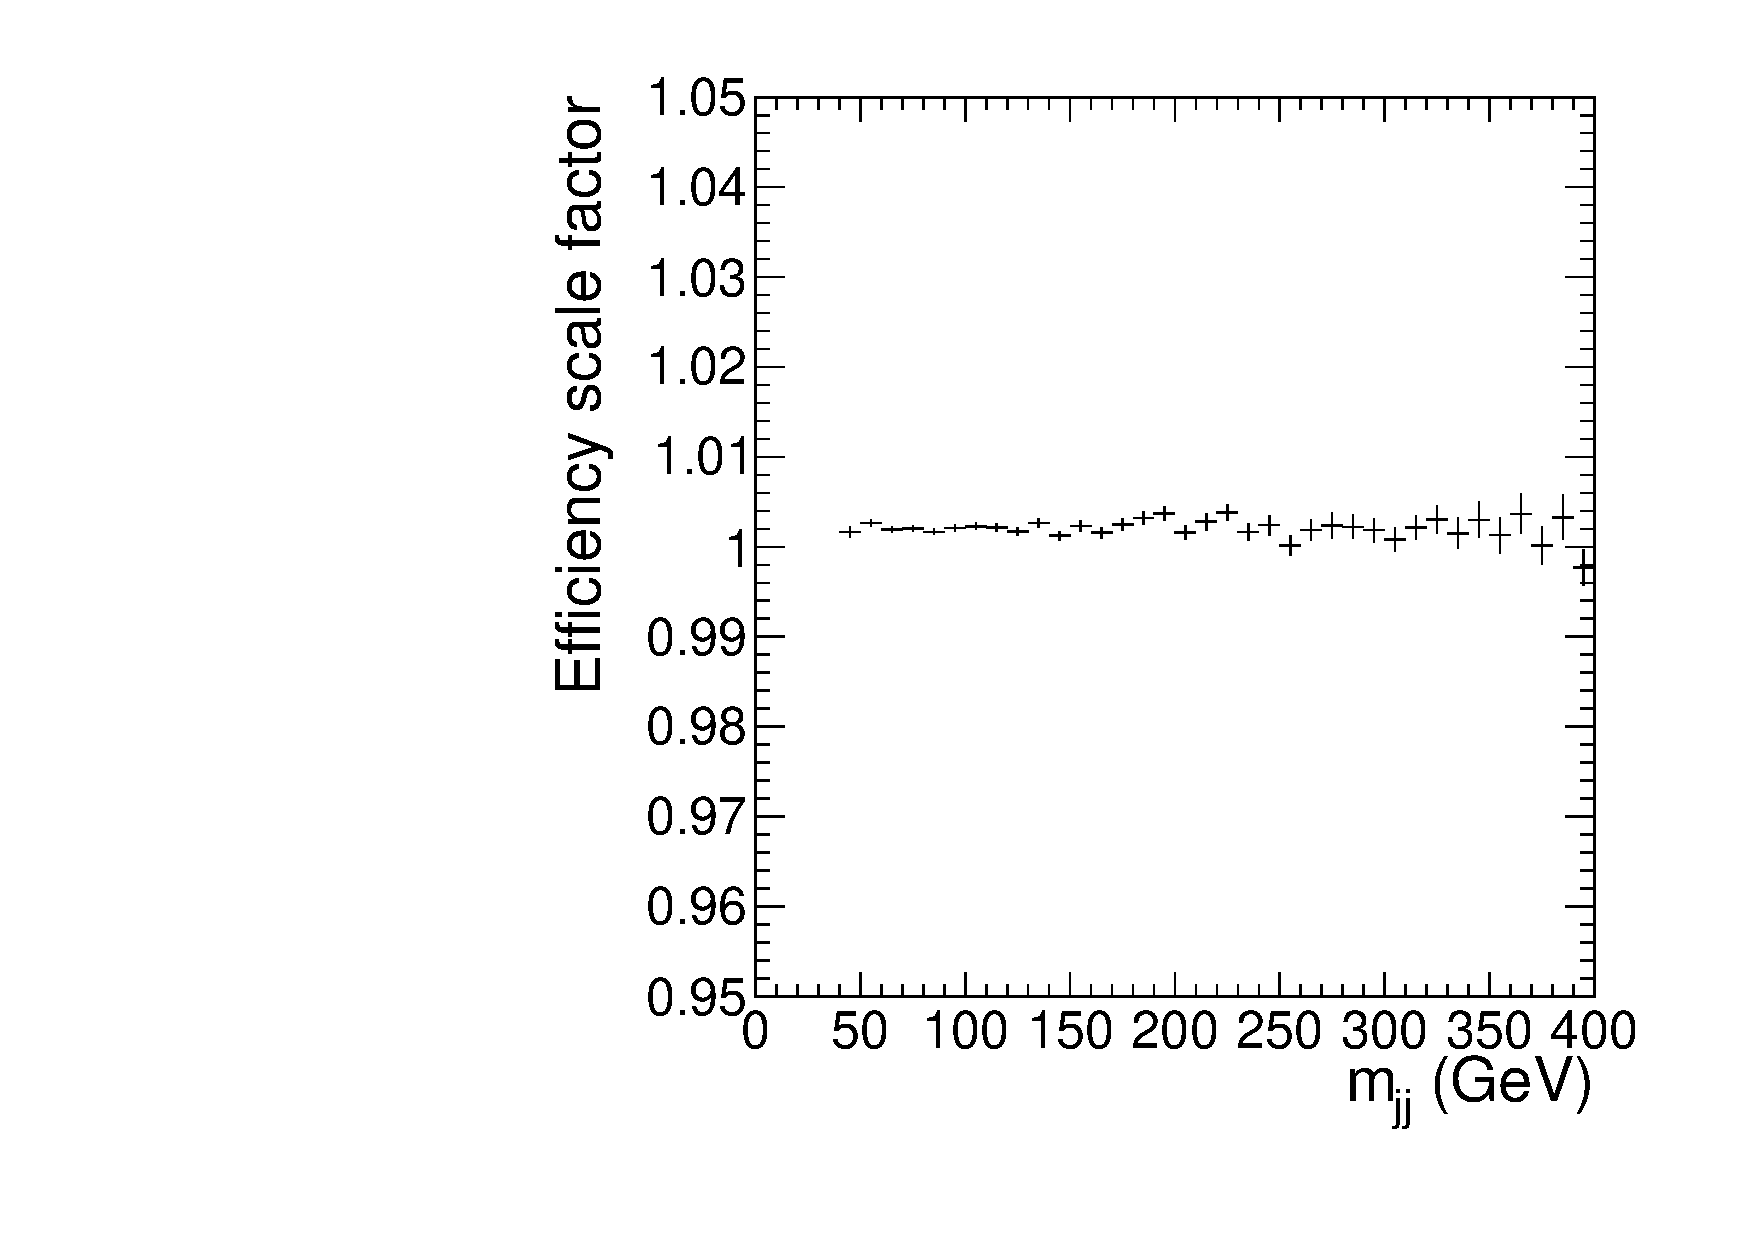
\includegraphics[width=0.48\textwidth]{figs/effPlots/fig_eff_ele_SCToReco_ScaleFactors.pdf}
   }
   \subfigure[]{
  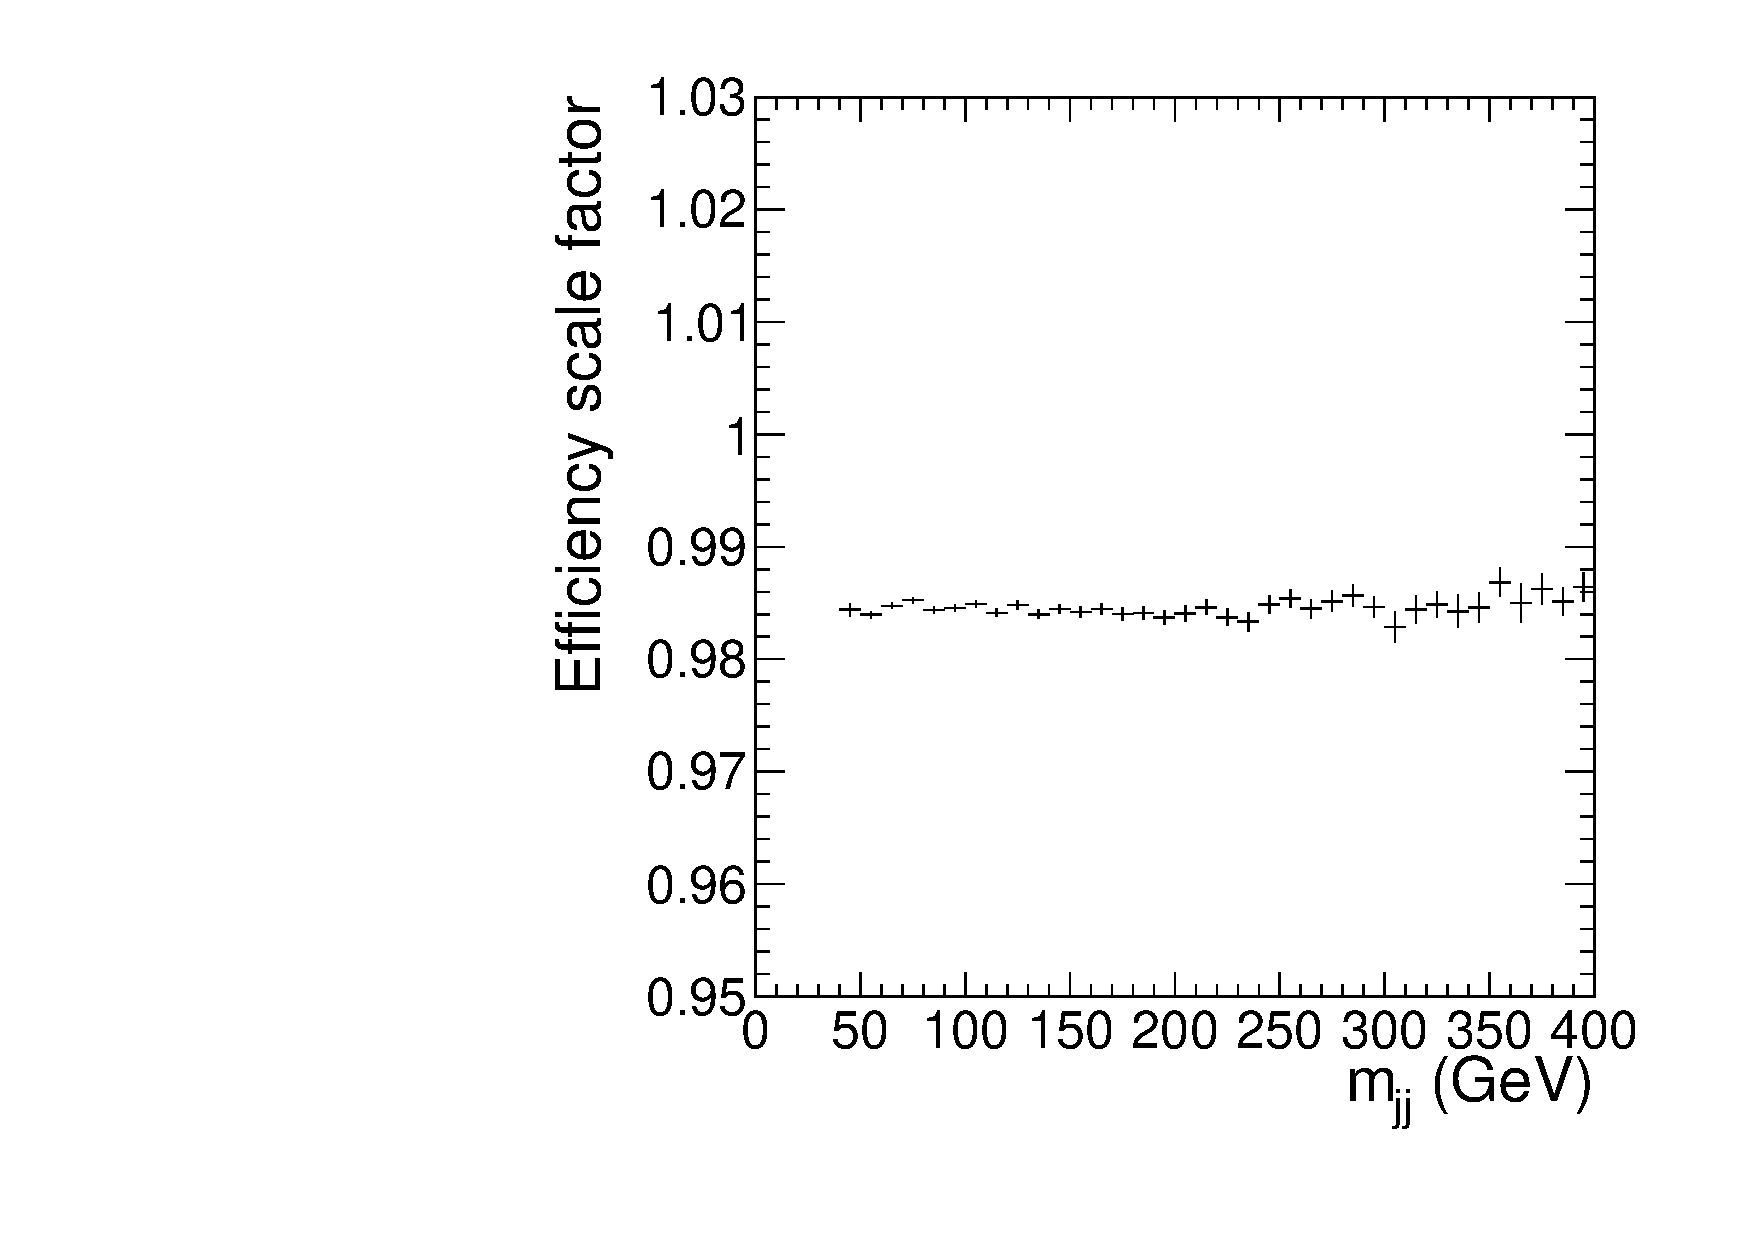
\includegraphics[width=0.48\textwidth]{figs/effPlots/fig_eff_ele_RecoToID_ScaleFactors.pdf}
   }
   \caption{Luminosity weighted average efficiency scale factors (data/MC) for electron 
   reconstruction, \textit{i.e.}, super cluster $\to$ GSF electron (a) and electron ID (b).}
\label{fig:electronRecoIDeffsf}}
\end{figure}
%%%%%%%%%%%%%%%%%%%%
%%%%%%%%%%%%%%%%%%%%%%%%%%%%%
\subsection{Electron selection (isolation and ID) scale factors}
The efficiency scale factor for electron selection is given in 
Table~\ref{tab:eleEffsRecoToWP80_ScaleFactors}.
The scale factor is statistically consistent with unity in the ECAL barrel and in the endcaps 
within systematic uncertainties.
Figure~\ref{fig:electronRecoIDeffsf} shows this scale factor variation in $m_{jj}$.
%%%%%%%%%%%
%\verbatiminput{eleEffsRecoToWP80_ScaleFactors.txt}
%%%%%%%%%%%%%%%%%%%%%%%%%%%%%
\begin{table}[bthp]
\begin{center}
  \begin{tabular}{l l c | l c}
    \hline  \hline
    $p_T$ range (GeV) & $\eta$ range  &
    $\frac{\epsilon_{\rm{Data}}}{\epsilon_{\rm{MC}}}$ & 
    $\eta$ range  & $\frac{\epsilon_{\rm{Data}}}{\epsilon_{\rm{MC}}}$\\
    \hline  
    30--35 &	-2.5-- -1.5 & 0.9937 $\pm$ 0.0073 & 1.5--2.5 & 0.9372 $\pm$ 0.0074 \\
           &	-1.5-- 0.0  & 1.0018 $\pm$ 0.0009 & 0.0--1.5 & 0.9958 $\pm$ 0.0039 \\
    \hline  
    35--40 &	-2.5-- -1.5 & 0.9545 $\pm$ 0.0055 & 1.5--2.5 & 0.9607 $\pm$ 0.0053 \\
           &	-1.5-- 0.0  & 0.9910 $\pm$ 0.0024 & 0.0--1.5 & 0.9960 $\pm$ 0.0025 \\
    \hline  
    40--45 &	-2.5-- -1.5 & 0.9661 $\pm$ 0.1567 & 1.5--2.5 & 0.9648 $\pm$ 0.0024 \\
           &	-1.5-- 0.0  & 0.9946 $\pm$ 0.0019 & 0.0--1.5 & 0.9892 $\pm$ 0.0877 \\
    \hline  
    45--50 &	-2.5-- -1.5 & 0.9672 $\pm$ 0.0050 & 1.5--2.5 & 0.9729 $\pm$ 0.0051 \\
           &	-1.5-- 0.0  & 0.9938 $\pm$ 0.0773 & 0.0--1.5 & 0.9917 $\pm$ 0.0022 \\
    \hline  
    50--200&	-2.5-- -1.5 & 0.9836 $\pm$ 0.0066 & 1.5--2.5 & 0.9813 $\pm$ 0.0068 \\
           &	-1.5-- 0.0  & 0.9915 $\pm$ 0.0030 & 0.0--1.5 & 0.9857 $\pm$ 0.0030 \\
    \hline  \hline
  \end{tabular}
\end{center}
\caption{\label{tab:eleEffsRecoToWP80_ScaleFactors}
Electron selection efficiency data/MC scale factors. The uncertainties are statistical only.}
\end{table}
%%%%%%%%%%%%%%%%%%%%%%%%%%%%%%%%%%%%%%%%%%%%%%%%%%%%%%%%%%%%%%%%%%%%
%%%%%%%%%%%%%%%%%%%%%%%%%%%%%%%%%%%%%%%%%%%%%%%%%%%%%%%%%%%%%%%%%%%%
%%%%%%%%%%%%%%%%%%%%%%%%%%%%%%%%%%%%%%%%%%%%%%%%%%%%%%%%%%%%%%%%%%%%
\section{Trigger selection}
\label{sec:trigger}
%%%%%%%%%%%%%%%%%%%%%%%%%%%%%%%
%%%%%%%%%%%%%%%%%%%%%%%%%%%%%%%
\subsection{Run2010: Runs 136033--149442}
\begin{itemize}
\item
Muon data:\\
     Mu9 OR Mu11 OR Mu13 OR Mu15\_v* OR Mu17\_v* OR Mu24\_v*  
\item
Electron data:\\   
     Ele10\_* OR Ele15\_* OR Ele17\_* 
\end{itemize}
%%%%%%%%%%%%%%%%%%%%%%%%%%%%%%%
%%%%%%%%%%%%%%%%%%%%%%%%%%%%%%%
\subsection{Run2011A: Menus 5E32 (Runs: 160404--163869), 
1E33 (Runs:165088--166967), and 1.4E33 (Runs:167039--167913)}
\begin{itemize}
\item
Muon data:\\
     IsoMu17\_v* OR Mu30\_v* \\
Note: We really needed to OR in the nonisolated muon 
trigger as it recovers about half of the offline-isolated 
muons rejected by IsoMu, increasing the trigger efficiency 
by ~5\%. 
\item
Electron data:\\   
Ele27\_CaloIdVT\_CaloIsoT\_TrkIdT\_TrkIsoT\_v* \, \, \, \textcolor{red}{5E32 epoch}\\
Ele25\_WP80\_PFMT40\_v1 \, \, \, \textcolor{red}{1E33 epoch}\\
Ele27\_WP80\_PFMT50\_v* \, \, \, \textcolor{red}{1.4E33 epoch}
\end{itemize}
%%%%%%%%%%%%%%%%%%%%%%%%%%%%%%%
%%%%%%%%%%%%%%%%%%%%%%%%%%%%%%%
\subsection{Run2011A:Menu 2E33, Runs 170249--173198}
\begin{itemize}
\item
Muon data:\\
     (IsoMu17\_v13 OR IsoMu20\_v8 OR IsoMu24\_v8) \, \, OR \, \, (Mu30\_v7 OR Mu40\_v5)\\

Note: This epoch was complicated because Mu30, IsoMu17, 
and IsoMu20 were all prescaled for brief periods, so we 
could either break it down into sub-epochs or lump them 
together. We chose the latter because it is predominantly 
IsoMu17 and the sub-epoch lumi accounting is painful.   
\item
Electron data:\\   
Ele27\_WP80\_PFMT50\_v*
\end{itemize}
%%%%%%%%%%%%%%%%%%%%%%%%%%%%%%%
%%%%%%%%%%%%%%%%%%%%%%%%%%%%%%%
\subsection{Run2011A:Menu 3E33, Runs: 173236--173692}
\begin{itemize}
\item
Muon data:\\
HLT\_IsoMu20\_v9 OR HLT\_Mu40\_eta2p1\_v1
\item
Electron data:\\
 Ele27\_WP80\_PFMT50\_v*
\end{itemize}
%%%%%%%%%%%%%%%%%%%%%%%%%%%%%%%
%%%%%%%%%%%%%%%%%%%%%%%%%%%%%%%
\subsection{Run2011B: Menu 3E33, Runs: 175832--178380}
\begin{itemize}
\item
Muon data:\\
    (IsoMu30\_eta2p1\_v3  OR IsoMu24\_eta2p1\_v3  OR IsoMu24\_v9 OR IsoMu20\_v9) \\
     OR \\  
    (Mu40\_eta2p1\_v1  OR  HLT\_Mu40\_v6)
\item
Electron data:\\  
Ele27\_WP80\_PFMT50\_v* OR Ele27\_WP70\_PFMT50\_v*
\end{itemize}
%%%%%%%%%%%%%%%%%%%%%%%%%%%%%%%
%%%%%%%%%%%%%%%%%%%%%%%%%%%%%%%
\subsection{Run2011B: Menu 5E33, Runs: 178420--180252}
\begin{itemize}
\item
Muon data:\\
       (IsoMu30\_eta2p1\_v6 OR IsoMu24\_eta2p1\_v6 OR IsoMu24\_v12 OR \\
       IsoMu30\_eta2p1\_v7 OR IsoMu24\_eta2p1\_v7 OR IsoMu24\_v13) \\
       OR \\
      (Mu40\_eta2p1\_v4 OR  Mu40\_v9) \, \, \,
      \textcolor{red}{(v1.4, 178420-179889)} \\
       OR (Mu40\_eta2p1\_v5 OR  Mu40\_v10) \, \, \,
      \textcolor{red}{(v2.2, 179959--180252)}
\item
Electron data:\\
 Ele32\_WP70\_PFMT50\_v*
\end{itemize}
%%%%%%%%%%%%%%%%%%%%%%%%%%%%%%%%%%%%%%%%%%%%%%%%%%%%%%%%%%%
\section{Trigger efficiency computation}
\label{sec:trigeff}
%%%%%%%%%%%%%%%%%%%%%%%%%%%%%%%%%%%%%%%%%%%%%%%%%%%%%%%%%%%
The efficiency of the single lepton triggers are computed 
using tag \& probe technique from Z$\to\ell^+\ell^-$ events.
The procedure is straightforward and is described in detail 
in \cite{tagnprobe} and \cite{eleceff}.
%%%%%%%%%%%%%%%%%%%%%%%%%%%%%%%%%%%%%%%%%%%%%%%%%%%%%%%%%%
\subsection{Muon trigger efficiency table}
\label{sec:trigeff_mu}
The luminosity weighted average (LWA) trigger efficiency 
for single muon triggers in data is given 
in Table~\ref{tab:muonEffsIsoToHLT_data_LP_LWA}. 
The efficiency is slowly varying
with changes in lepton transverse momentum and rapidity. 
The efficiency is typically
about 90\%.
%%%%%%%%%%%
%\verbatiminput{muonEffsIsoToHLT_data_LP_LWA.txt}
%%%%%%%%%%%%%%%%%%%%%%%%%%%%%
\begin{table}[bthp]
\begin{center}
  \begin{tabular}{l l c | l c}
    \hline  \hline
    $p_T$ range (GeV) & $\eta$ range  & $\epsilon_{\rm{Data}}$ & 
    $\eta$ range  & $\epsilon_{\rm{Data}}$\\
    \hline  
    25--30 &	-2.1-- -1.5 &	0.8490 $\pm$ 0.0032  & 1.5--2.1   & 0.8457 $\pm$ 0.0033 \\
           &	-1.5-- -1.0 &	0.8725 $\pm$ 0.0032  & 1.0--1.5   & 0.8628 $\pm$ 0.0032 \\
           &	-1.0-- -0.5 &	0.9057 $\pm$ 0.0026  & 0.5--1.0   & 0.8999 $\pm$ 0.0027 \\
           &	-0.5--	0.0 &	0.9211 $\pm$ 0.0022  & 0.0--0.5   & 0.9251 $\pm$ 0.0022 \\
    \hline  
    30--35 &	-2.1-- -1.5 &	0.8797 $\pm$ 0.0031  & 1.5--2.1   & 0.8768 $\pm$ 0.0031 \\
           &	-1.5-- -1.0 &	0.9136 $\pm$ 0.0030  & 1.0--1.5   & 0.9016 $\pm$ 0.0031 \\
           &	-1.0-- -0.5 &	0.9397 $\pm$ 0.0025  & 0.5--1.0   & 0.9387 $\pm$ 0.0025 \\
           &	-0.5--	0.0 &	0.9579 $\pm$ 0.0022  & 0.0--0.5   & 0.9556 $\pm$ 0.0021 \\
    \hline  
    35--40 &	-2.1-- -1.5 &	0.8816 $\pm$ 0.0027  & 1.5--2.1   & 0.8894 $\pm$ 0.0026 \\
           &	-1.5-- -1.0 &	0.9142 $\pm$ 0.0025  & 1.0--1.5   & 0.9008 $\pm$ 0.0026 \\
           &	-1.0-- -0.5 &	0.9385 $\pm$ 0.0022  & 0.5--1.0   & 0.9385 $\pm$ 0.0021 \\
           &	-0.5--	0.0 &	0.9571 $\pm$ 0.0019  & 0.0--0.5   & 0.9546 $\pm$ 0.0019 \\
    \hline  
    40--45 &	-2.1-- -1.5 &	0.8878 $\pm$ 0.0024  & 1.5--2.1   & 0.8902 $\pm$ 0.0024 \\
           &	-1.5-- -1.0 &	0.9221 $\pm$ 0.0021  & 1.0--1.5   & 0.9076 $\pm$ 0.0022 \\
           &	-1.0-- -0.5 &	0.9443 $\pm$ 0.0020  & 0.5--1.0   & 0.9457 $\pm$ 0.0019 \\
           &	-0.5--	0.0 &	0.9622 $\pm$ 0.0018  & 0.0--0.5   & 0.9617 $\pm$ 0.0018 \\
    \hline  
    45--50 &	-2.1-- -1.5 &	0.8922 $\pm$ 0.0029  & 1.5--2.1   & 0.8934 $\pm$ 0.0028 \\
           &	-1.5-- -1.0 &	0.9202 $\pm$ 0.0027  & 1.0--1.5   & 0.9069 $\pm$ 0.0027 \\
           &	-1.0-- -0.5 &	0.9458 $\pm$ 0.0024  & 0.5--1.0   & 0.9437 $\pm$ 0.0025 \\
           &	-0.5--	0.0 &	0.9625 $\pm$ 0.0023  & 0.0--0.5   & 0.9615 $\pm$ 0.0023 \\
    \hline  
    50--200&	-2.1-- -1.5 &	0.8920 $\pm$ 0.0031  & 1.5--2.1   & 0.8903 $\pm$ 0.0032 \\
           &	-1.5-- -1.0 &	0.9178 $\pm$ 0.0030  & 1.0--1.5   & 0.9041 $\pm$ 0.0030 \\
           &	-1.0-- -0.5 &	0.9419 $\pm$ 0.0027  & 0.5--1.0   & 0.9424 $\pm$ 0.0028 \\
           &	-0.5--	0.0 &	0.9606 $\pm$ 0.0026  & 0.0--0.5   & 0.9604 $\pm$ 0.0025 \\
    \hline  \hline
  \end{tabular}
\end{center}
\caption{\label{tab:muonEffsIsoToHLT_data_LP_LWA}
Muon trigger efficiency in data (luminosity 
weighted average). The uncertainties are statistical only.}
\end{table}
%%%%%%%%%%%%
%%%%%%%%%%%
\subsection{Electron trigger efficiency table}
\label{sec:trigeff_eleEle27}
The luminosity weighted average trigger efficiency for the 
electron leg of the single electron triggers is shown in
Table~\ref{tab:eleEffsHLTEle}.  
The value is typically about 99\% in the barrel and 92--97\% in 
the endcaps, and is weakly dependent on the electron
$p_T$ and pseudorapidity.
The efficiency for the W transverse mass leg is shown in 
Table~\ref{tab:eleEffsHLTEleMT}.  
The average value is 91.74 $\pm$ 0.07\% with a large variation depending on 
whether the electron is in the barrel or endcaps.
Fortunately for us this is just an overall scaling effect in the 
$m_{jj}$ and $m_{\ell\nu jj}$ distributions.
The impact of this turnon on the dijet invariant mass templates
(used in Higgs analysis) is negligible, as shown in 
Figs.~\ref{fig:muonhlteff}-\ref{fig:singleElehlteffMT}.

%%%%%%%%%%%
%\verbatiminput{eleEffsWP80ToHLTEle27_May10ReReco.txt}
%%%%%%%%%%%%%%%%%%%%%%%%%%%%%%
%\begin{table}[bthp]
%\begin{center}
%  \begin{tabular}{l l c | l c}
%    \hline  \hline
%    $p_T$ range (GeV) & $\eta$ range  & $\epsilon_{\rm{Data}}$ & 
%    $\eta$ range  & $\epsilon_{\rm{Data}}$\\
%    \hline  
%    30--35 &	-2.5-- -1.5 & 0.96 $\pm$ 0.01 & 1.5--2.5 & 0.93 $\pm$ 0.01 \\
%           &	-1.5-- 0.0  & 0.97 $\pm$ 0.00 & 0.0--1.5 & 0.97 $\pm$ 0.00 \\
%    \hline  
%    35--40 &	-2.5-- -1.5 & 0.97 $\pm$ 0.00 & 1.5--2.5 & 0.97 $\pm$ 0.00 \\
%           &	-1.5-- 0.0  & 0.97 $\pm$ 0.00 & 0.0--1.5 & 0.97 $\pm$ 0.00 \\
%    \hline  
%    40--45 &	-2.5-- -1.5 & 0.97 $\pm$ 0.00 & 1.5--2.5 & 0.97 $\pm$ 0.00 \\
%           &	-1.5-- 0.0  & 0.98 $\pm$ 0.00 & 0.0--1.5 & 0.98 $\pm$ 0.00 \\
%    \hline  
%    45--50 &	-2.5-- -1.5 & 0.97 $\pm$ 0.00 & 1.5--2.5 & 0.97 $\pm$ 0.00 \\
%           &	-1.5-- 0.0  & 0.98 $\pm$ 0.00 & 0.0--1.5 & 0.98 $\pm$ 0.00 \\
%    \hline  
%    50--200&	-2.5-- -1.5 & 0.97 $\pm$ 0.01 & 1.5--2.5 & 0.98 $\pm$ 0.00 \\
%           &	-1.5-- 0.0  & 0.98 $\pm$ 0.00 & 0.0--1.5 & 0.98 $\pm$ 0.00 \\
%    \hline  \hline
%  \end{tabular}
%\end{center}
%\caption{\label{tab:eleEffsWP80ToHLTEle27_May10ReReco}
%Electron trigger efficiency in data for the Ele27 trigger in the May10ReReco dataset. 
%The uncertainties are statistical only.}
%\end{table}
%%%%%%%%%%%%%%%%%%%%%%%%%%%%%%%%%%%%%%%%%%%%%%%%%%%%%%%%%%%%%%%%%%%%%
%%%%%%%%%%%%%%%%%%%%%%%%%%%%%
\begin{table}[bthp]
\begin{center}
  \begin{tabular}{l l c | l c}
    \hline  \hline
    $p_T$ range (GeV) & $\eta$ range  & $\epsilon_{\rm{Data}}$ & 
    $\eta$ range  & $\epsilon_{\rm{Data}}$\\
    \hline  
    35--40 &	-2.5-- -1.5 & 0.92 $\pm$ 0.01 & 1.5--2.5 & 0.91 $\pm$ 0.01 \\
           &	-1.5-- 0.0  & 0.99 $\pm$ 0.01 & 0.0--1.5 & 0.99 $\pm$ 0.01 \\
    \hline  
    40--45 &	-2.5-- -1.5 & 0.96 $\pm$ 0.01 & 1.5--2.5 & 0.96 $\pm$ 0.01 \\
           &	-1.5-- 0.0  & 0.99 $\pm$ 0.01 & 0.0--1.5 & 0.99 $\pm$ 0.01 \\
    \hline  
    45--50 &	-2.5-- -1.5 & 0.97 $\pm$ 0.01 & 1.5--2.5 & 0.97 $\pm$ 0.01 \\
           &	-1.5-- 0.0  & 0.99 $\pm$ 0.01 & 0.0--1.5 & 0.99 $\pm$ 0.01 \\
    \hline  
    50--200&	-2.5-- -1.5 & 0.93 $\pm$ 0.01 & 1.5--2.5 & 0.92 $\pm$ 0.01 \\
           &	-1.5-- 0.0  & 0.98 $\pm$ 0.01 & 0.0--1.5 & 0.98 $\pm$ 0.01 \\
    \hline  \hline
  \end{tabular}
\end{center}
\caption{\label{tab:eleEffsHLTEle}
Electron trigger efficiency in data (luminosity weighted average). 
The uncertainties are statistical only.}
\end{table}
%%%%%%%%%%%%%%%%%%%%%%%%%%%%%
%%%%%%%%%%%%%%%%%%%%%%%%%%%%%
\begin{table}[bthp]
\begin{center}
  \begin{tabular}{l l c | l c}
    \hline  \hline
    Offline $m_T$ range (GeV) & electron $\eta$ range  & $\epsilon_{\rm{Data}}$ & 
    electron $\eta$ range  & $\epsilon_{\rm{Data}}$\\
    \hline  
     50--55 &	-2.5-- -1.5 & 0.3580 $\pm$ 0.0167 &	+1.5--2.5 & 0.3580 $\pm$ 0.0167 \\ 
            &	-1.5--0.0 & 0.7315 $\pm$ 0.0129  &	+0.0--1.5 & 0.7315 $\pm$ 0.0129 \\
    \hline
     55--60 &	-2.5-- -1.5 & 0.4796 $\pm$ 0.0165  &	+1.5--2.5 & 0.4796 $\pm$ 0.0165 \\ 
            &	-1.5--0.0 & 0.8151 $\pm$ 0.0112  &	+0.0--1.5 & 0.8151 $\pm$ 0.0112 \\ 
    \hline
     60--65 &	-2.5-- -1.5 & 0.6073 $\pm$ 0.0144  &	+1.5--2.5 & 0.6073 $\pm$ 0.0144 \\ 
            &	-1.5--0.0 & 0.9035 $\pm$ 0.0085  &	+0.0--1.5 & 0.9035 $\pm$ 0.0085 \\ 
    \hline
     65--70 &	-2.5-- -1.5 & 0.7473 $\pm$ 0.0100 &	+1.5--2.5 & 0.7473 $\pm$ 0.0100 \\  
            &	-1.5--0.0 & 0.9548 $\pm$ 0.0047  &	+0.0--1.5 & 0.9548 $\pm$ 0.0047  \\
    \hline
     70--75 &	-2.5-- -1.5 & 0.8256 $\pm$ 0.0069  &	+1.5--2.5 & 0.8256 $\pm$ 0.0069 \\ 
            &	-1.5--0.0 & 0.9756 $\pm$ 0.0036  &	+0.0--1.5 & 0.9756 $\pm$ 0.0036 \\ 
    \hline
     75--80 &	-2.5-- -1.5 & 0.8711 $\pm$ 0.0060  &	+1.5--2.5 & 0.8711 $\pm$ 0.0060 \\ 
            &	-1.5--0.0 & 0.9866 $\pm$ 0.0034  &	+0.0--1.5 & 0.9866 $\pm$ 0.0034 \\
    \hline
     80--85 &	-2.5-- -1.5 & 0.9047 $\pm$ 0.0059  &	+1.5--2.5 & 0.9047 $\pm$ 0.0059  \\
            &	-1.5--0.0 & 0.9934 $\pm$ 0.0034  &	+0.0--1.5 & 0.9934 $\pm$ 0.0034 \\ 
    \hline
     85--90 &	-2.5-- -1.5 & 0.9308 $\pm$ 0.0061  &	+1.5--2.5 & 0.9308 $\pm$ 0.0061 \\ 
            &	-1.5--0.0 & 0.9958 $\pm$ 0.0038  &	+0.0--1.5 & 0.9958 $\pm$ 0.0038  \\
    \hline
     90--95 &	-2.5-- -1.5 & 0.9415 $\pm$ 0.0068  &	+1.5--2.5 & 0.9415 $\pm$ 0.0068  \\
            &	-1.5--0.0 & 0.9975 $\pm$ 0.0046  &	+0.0--1.5 & 0.9975 $\pm$ 0.0046  \\
    \hline
     95--100 &	-2.5-- -1.5 & 0.9441 $\pm$ 0.0080 &	+1.5--2.5 & 0.9441 $\pm$ 0.0080  \\ 
             &	-1.5--0.0 & 0.9973 $\pm$ 0.0057  &	+0.0--1.5 & 0.9973 $\pm$ 0.0057  \\
    \hline
     100--110 &	-2.5-- -1.5 & 0.9358 $\pm$ 0.0074  &	+1.5--2.5 & 0.9358 $\pm$ 0.0074 \\ 
              &	-1.5--0.0 & 0.9980 $\pm$ 0.0059  &	+0.0--1.5 & 0.9980 $\pm$ 0.0059 \\ 
    \hline
     110--120 &	-2.5-- -1.5 & 0.9120 $\pm$ 0.0109  &	+1.5--2.5 & 0.9120 $\pm$ 0.0109 \\
              &	-1.5--0.0 & 0.9963 $\pm$ 0.0101  &	+0.0--1.5 & 0.9963 $\pm$ 0.0101  \\
    \hline
     120--140 &	-2.5-- -1.5 & 0.8721 $\pm$ 0.0117  &	+1.5--2.5 & 0.8721 $\pm$ 0.0117  \\
              &	-1.5--0.0 & 0.9950 $\pm$ 0.0123  &	+0.0--1.5 & 0.9950 $\pm$ 0.0123  \\
    \hline
     140--180 &	-2.5-- -1.5 & 0.8311 $\pm$ 0.0153  &	+1.5--2.5 & 0.8311 $\pm$ 0.0153  \\
              &	-1.5--0.0 & 0.9899 $\pm$ 0.0171  &	+0.0--1.5 & 0.9899 $\pm$ 0.0171  \\
    \hline
     180--240 &	-2.5-- -1.5 & 0.8011 $\pm$ 0.0266  &	+1.5--2.5 & 0.8011 $\pm$ 0.0266  \\
              &	-1.5--0.0 & 0.9915 $\pm$ 0.0290  &	+0.0--1.5 & 0.9915 $\pm$ 0.0290  \\
    \hline
     240--300 &	-2.5-- -1.5 & 0.8110 $\pm$ 0.0710  &	+1.5-+2.5 & 0.8110 $\pm$ 0.0710 \\ 
              &	-1.5--0.0 & 1.0000 $\pm$ 0.0829  &	+0.0--1.5 & 1.0000 $\pm$ 0.0829  \\
    \hline  \hline
  \end{tabular}
\end{center}
\caption{\label{tab:eleEffsHLTEleMT}
Efficiency for W transverse mass cut ($> 50$~GeV for most epochs) in HLT 
for single electron trigger in data (luminosity weighted average). 
The uncertainties are all inclusive.}
\end{table}
%%%%%%%%%%%%%%%%%%%%%%%%%%%%%
%%%%%%%%%%%%%%%%%%%%%%%%%%%%%%%%%%%%%%%%%%%%%%%%%%%%%%%%%%%%%%%%%%%%
%%%%%%%%%%%%%%%%%%%%%%%%%%%%%%%%%%%%%%%
\subsection{Effect of trigger efficiency on shapes}
As shown in Figs.~\ref{fig:muonhlteff}-\ref{fig:singleElehlteffMT}, 
the overall trigger efficiency with respect to the analysis selection criteria
is uniform 
across various trigger epochs within the systematic uncertainty. 
Since the trigger efficiency is flat, it does not alter the 
di-jet mass shape, other than introducing a 
global factor that will be absorbed in the normalization of the fit.
Therefore, we have followed the strategy not to apply any trigger 
correction in Monte Carlo. 
We compute the systematic error due to the efficiency 
uncertainty by recomputing the envelope for the MC shape templates 
and propagating these templates to the $m_{jj}$ fit as described in 
a later section. 
%%%%%%%%%%%%%%%%%%%%
\begin{figure}[h!t]
  {\centering
  \subfigure[]{
  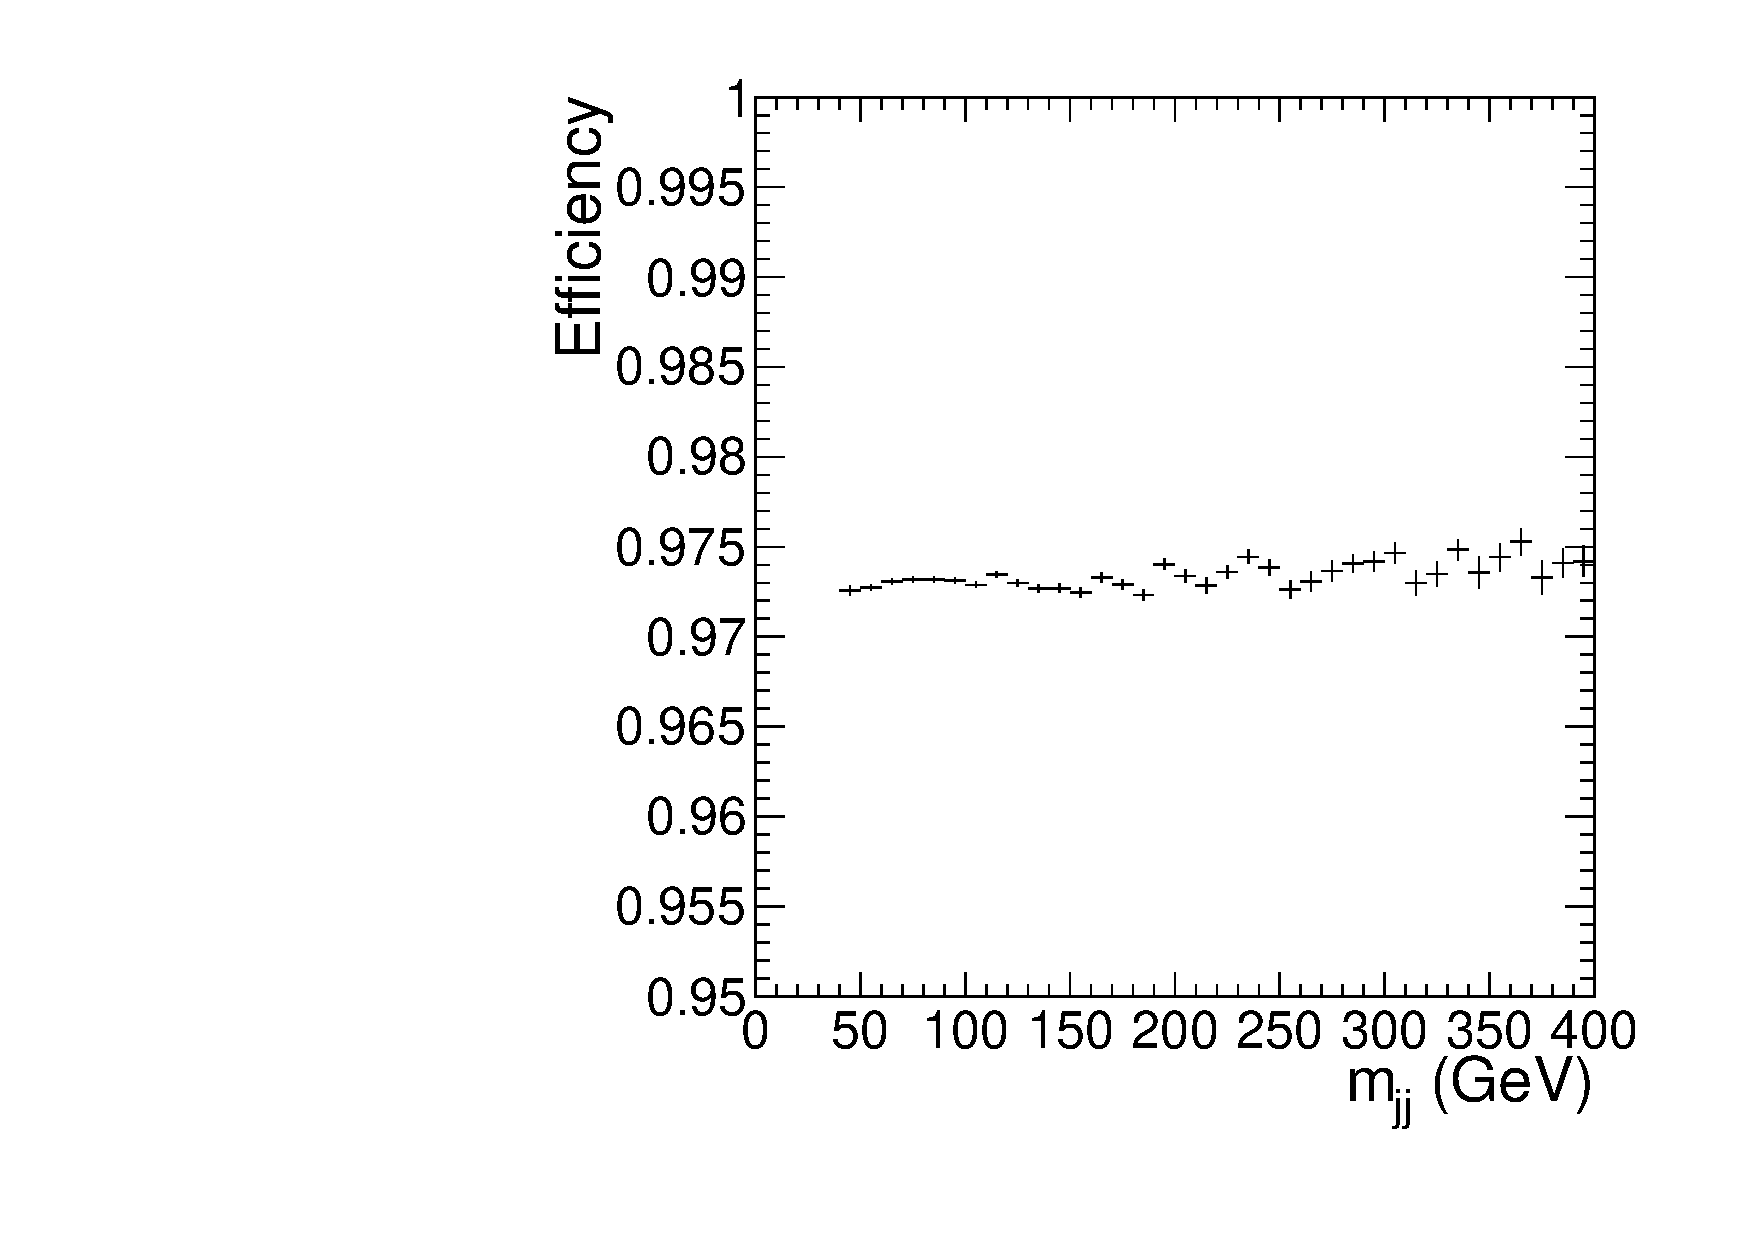
\includegraphics[width=0.48\textwidth]{figs/effPlots/fig_eff_HLTMu.pdf}
  }   
  \subfigure[]{
  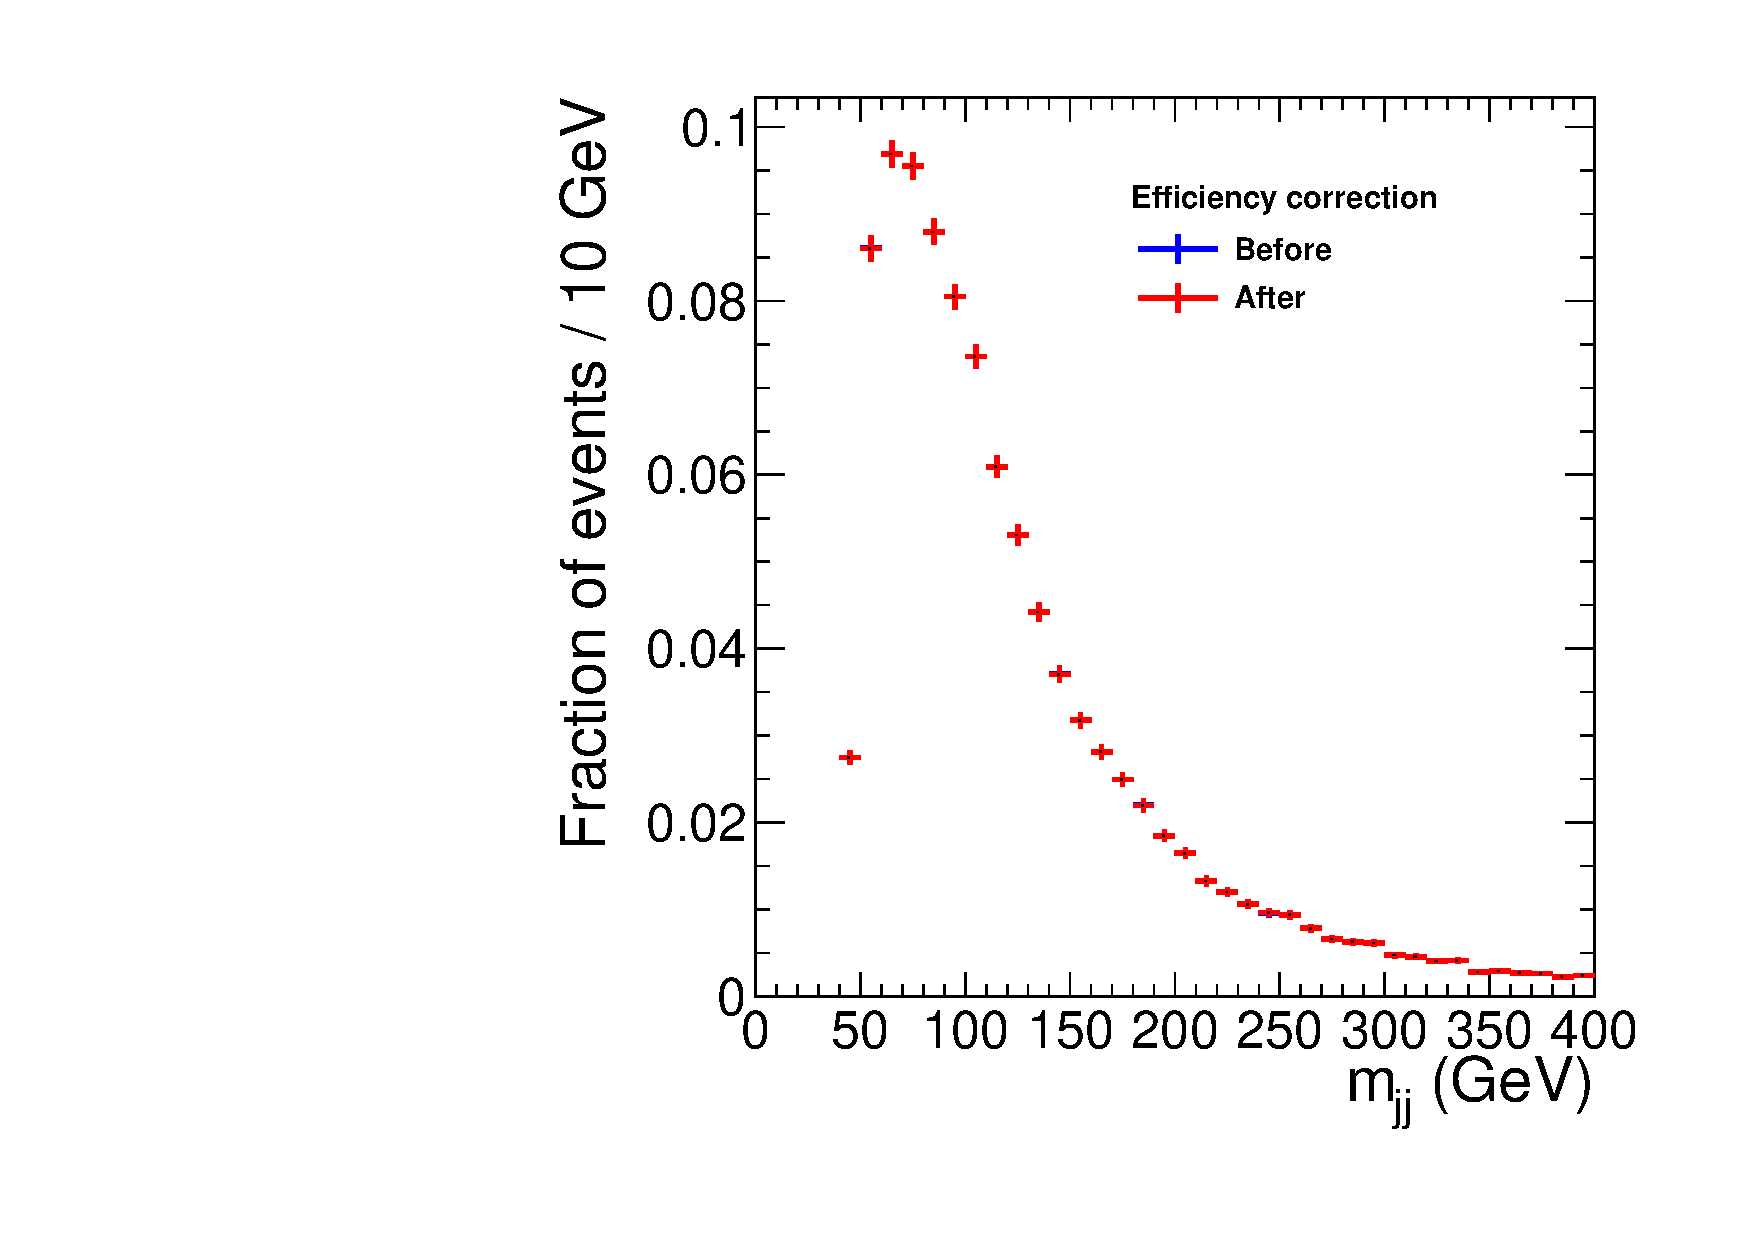
\includegraphics[width=0.48\textwidth]{figs/effPlots/fig_eff_HLTMu_template.pdf}
   }
   \caption{Luminosity weighted average trigger efficiency in the muon data as a function 
   of $m_{jj}$ (a). 
   The effect of this efficiency correction on W+jets $m_{jj}$ shape (b).}
\label{fig:muonhlteff}}
\end{figure}
%%%%%%%%%%%%%%%%%%%%
%%%%%%%%%%%%%%%%%%%%
\begin{figure}[h!t]
  {\centering
  \subfigure[]{
  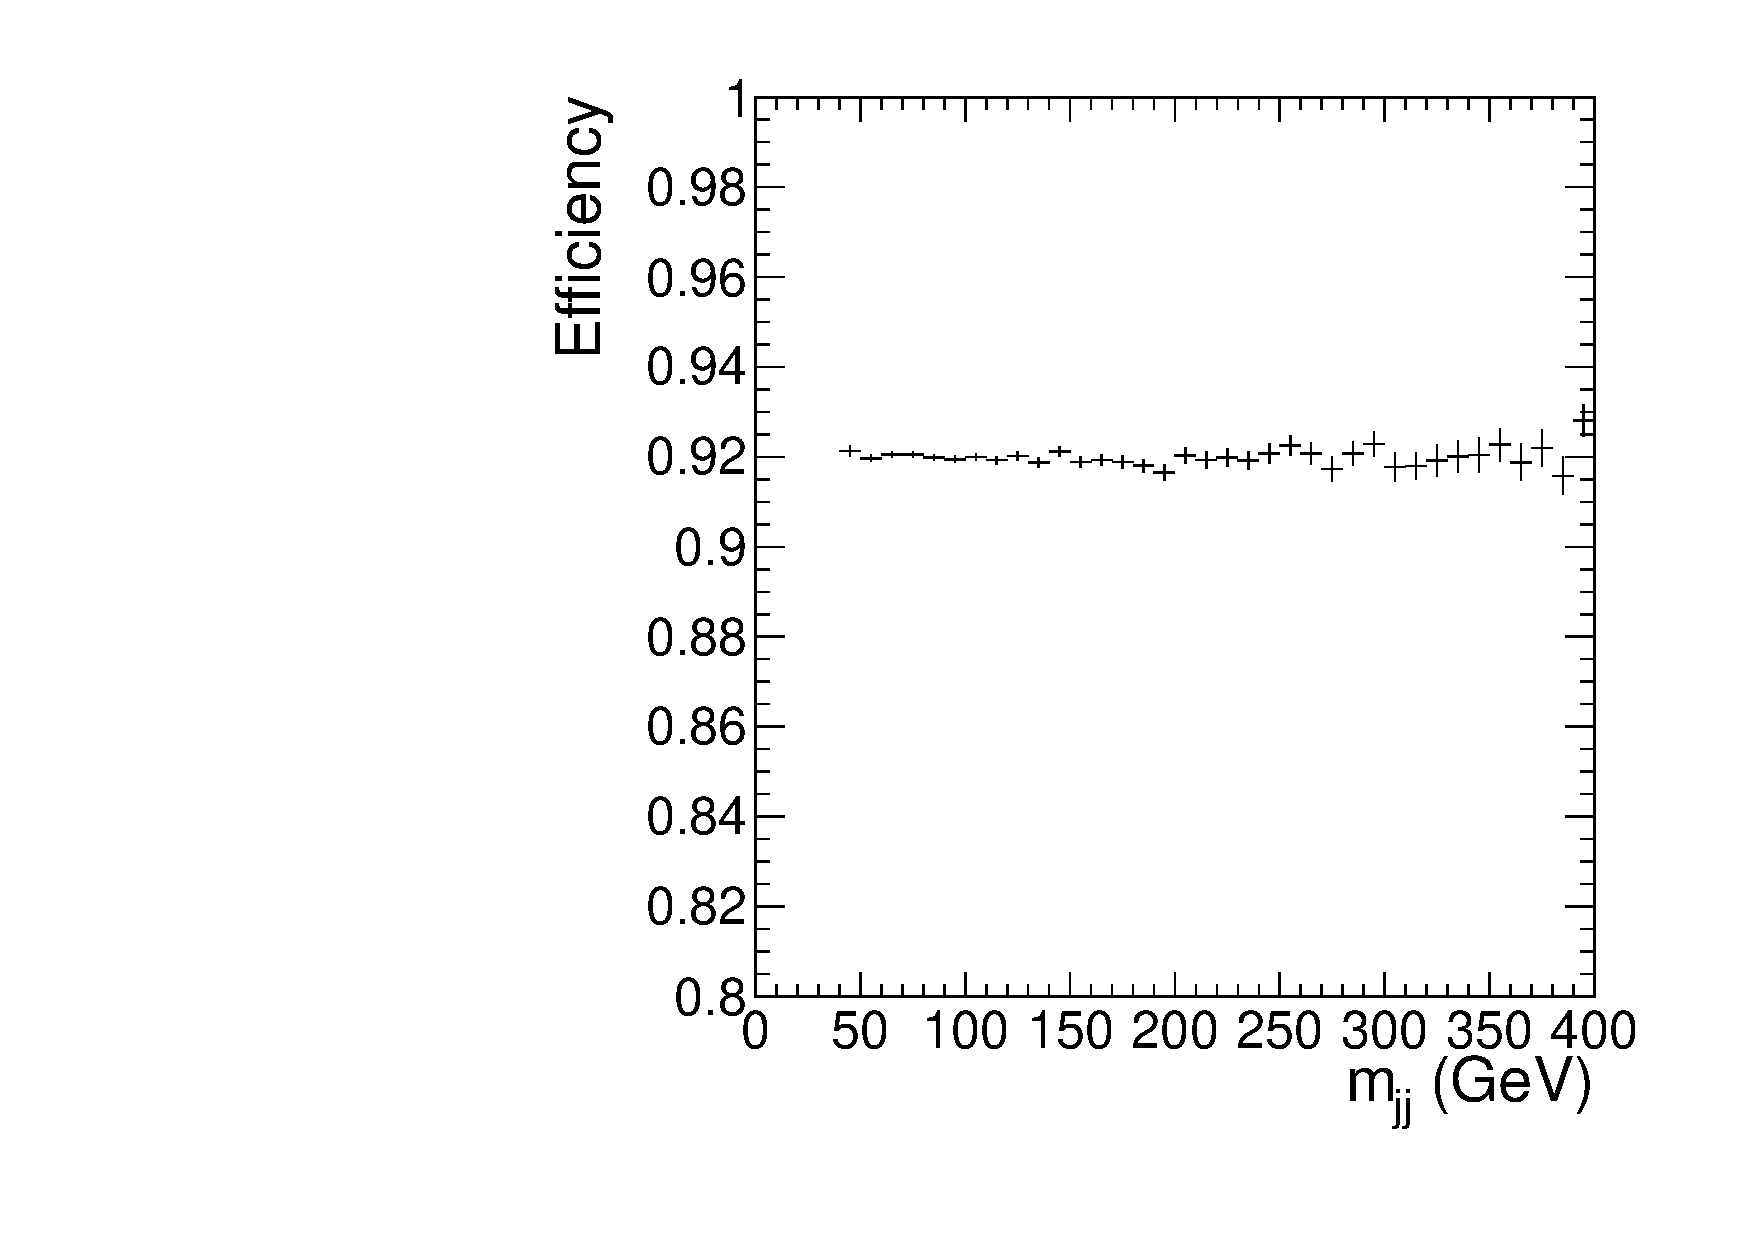
\includegraphics[width=0.48\textwidth]{figs/effPlots/fig_eff_HLTEle27_May10ReReco.pdf}
  }   
  \subfigure[]{
  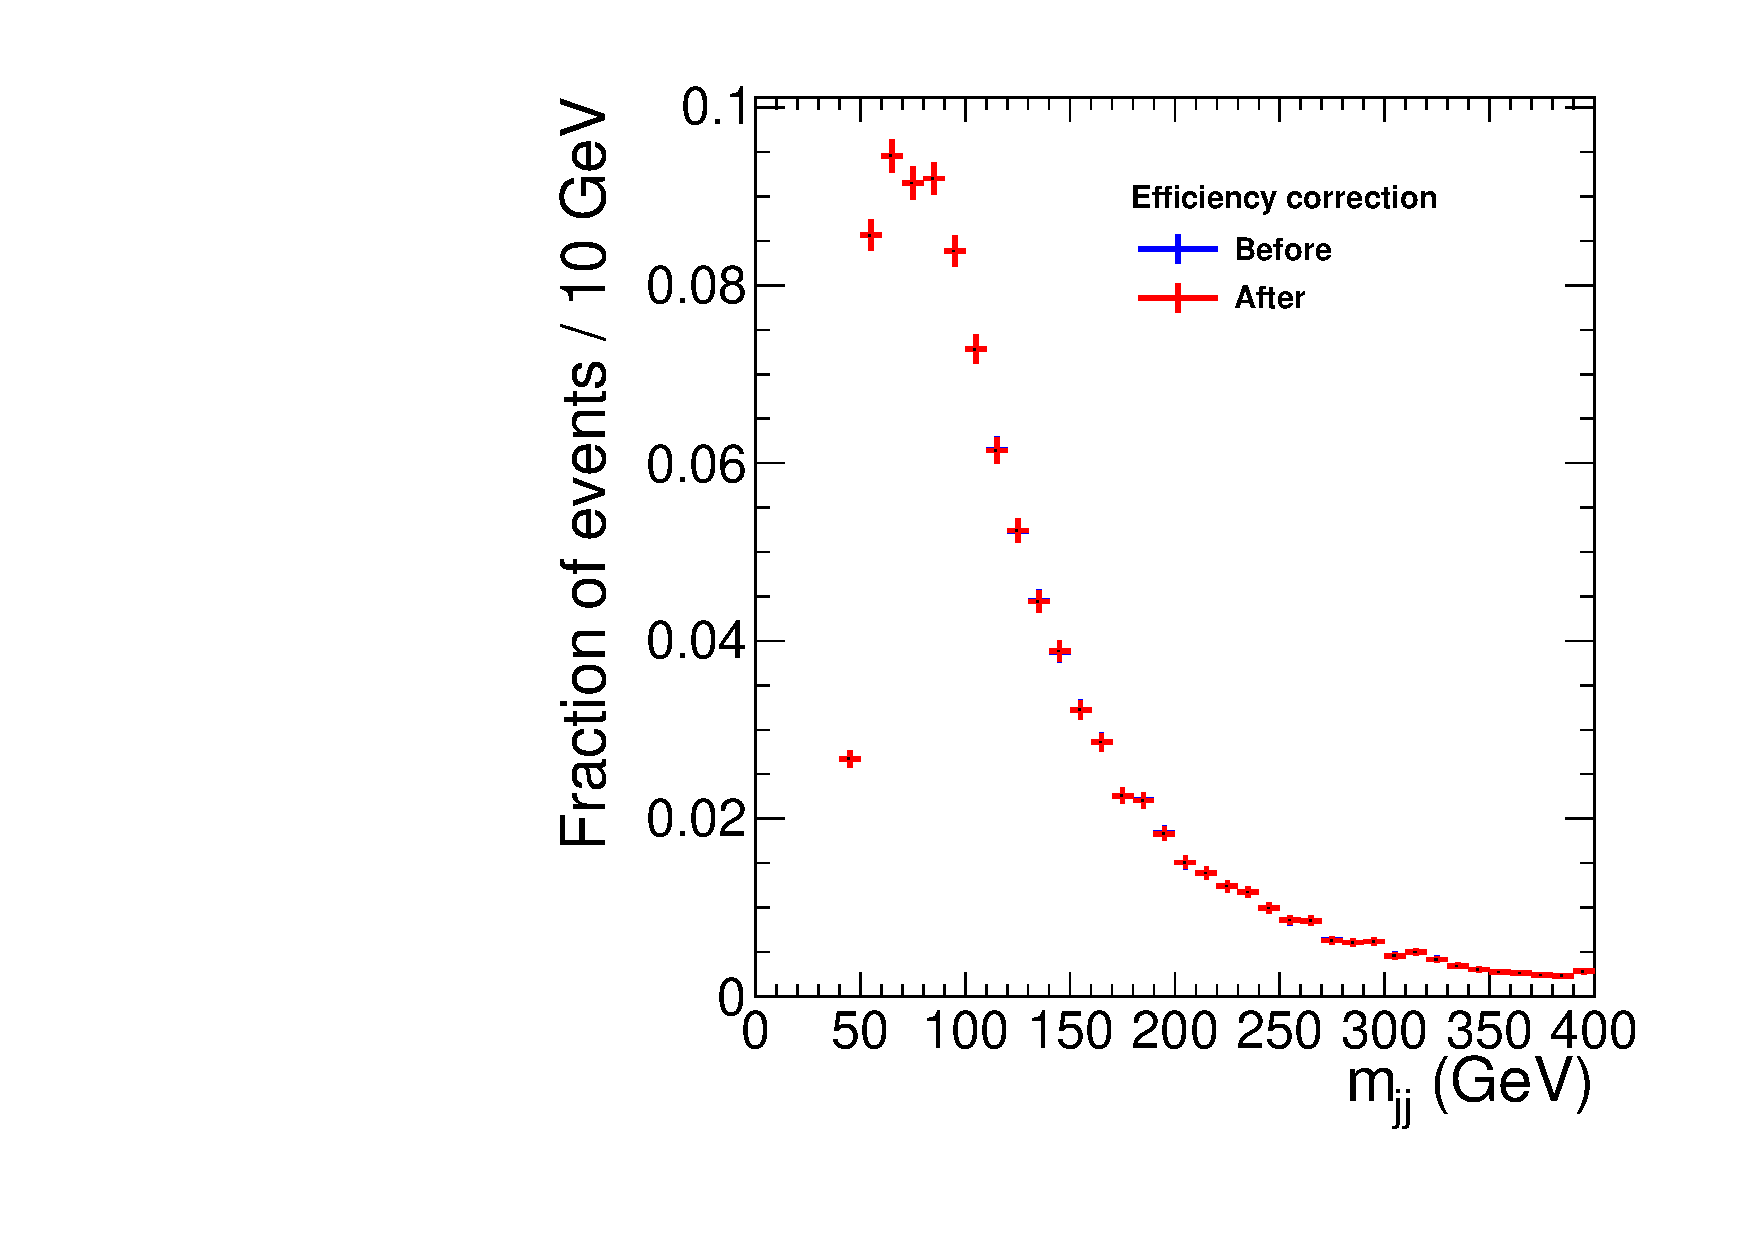
\includegraphics[width=0.48\textwidth]{figs/effPlots/fig_eff_HLTEle27_May10ReReco_template.pdf}
   }
   \caption{Luminosity weighted average trigger efficiency in the 
   %first 200 pb${}^{-1}$ of 2011 electron data (single electron $HLT_Ele27$) 
     electron data for single electron leg as a function 
   of $m_{jj}$ (a). 
   The effect of this efficiency correction on W+jets $m_{jj}$ shape (b).}
\label{fig:singleElehlteff}}
\end{figure}
%%%%%%%%%%%%%%%%%%%%
%%%%%%%%%%%%%%%%%%%%
\begin{figure}[h!t]
  {\centering
  \subfigure[]{
  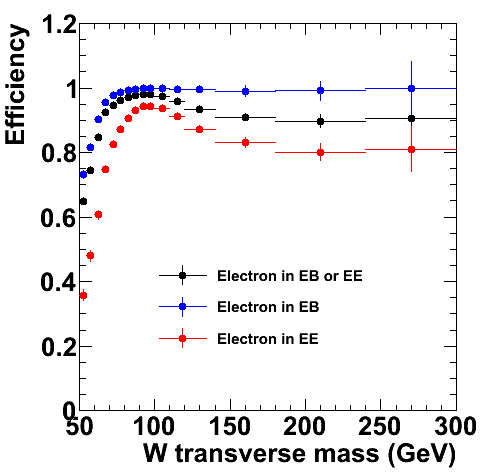
\includegraphics[width=0.48\textwidth]{figs/effPlots/WMt50TriggerEfficiency.png}
  }   
  \subfigure[]{
  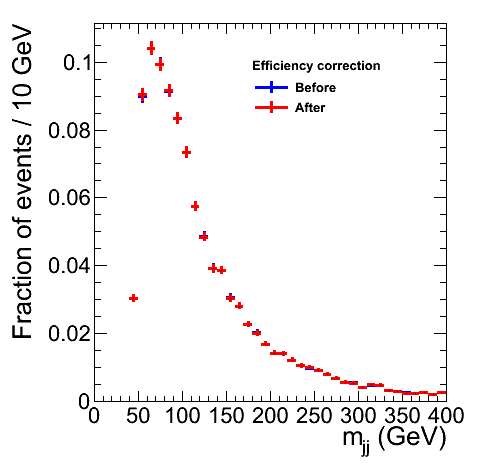
\includegraphics[width=0.48\textwidth]{figs/effPlots/fig_eff_HLTWMT50_template.png}
   }
   \caption{Luminosity weighted average trigger efficiency in the 
   %first 200 pb${}^{-1}$ of 2011 electron data (single electron $HLT_Ele27$) 
     electron data for W transverse mass leg as a function 
   of $m_{jj}$ (a). 
   The effect of this efficiency correction on W+jets $m_{jj}$ shape (b).}
\label{fig:singleElehlteffMT}}
\end{figure}
%%%%%%%%%%%%%%%%%%%%
%%%%%%%%%%%%%%%%%%%%%%%%%%%%%%%%%%%%%%%
\subsection{Effect of trigger efficiency on yields}
The signal templates are corrected event-by-event for trigger 
efficiency. Since the efficiency is high (90--100\%) with weak  
dependence on lepton kinematics, the overall effect is small. 
The background yields remain unaffected by the absolute value 
of the trigger efficiency because the background yields are 
allowed to float in the fit.
%%%%%%%%%%%%%%%%%%%%%%%%%%%%%%%%%%%%%%%%%%%%%%%%%%%%%%%%%%%%%%%%%%%%
%%%%%%%%%%%%%%%%%%%%%%%%%%%%%%%%%%%%%%%%%%%%%%%%%%%%%%%%%%%%%%%%%%%%
\clearpage
\section{Effect of pileup}
\label{sec:pileup}
The presence of additional interactions, known as Pile-up (PU), is expected to affect
this analysis in the following ways:
%%%%%
\begin{itemize}
\item additional energy deposits from PU will be added to the jets from the main 
interaction
\item additional low $p_{T}$ jets composed of PU energy will be
added to the event
\item tracks and calorimetric towers from PU energy deposits will be
added to the isolation energy sum of the lepton, thus making isolation 
cuts less efficient.
\end{itemize}
%%%%%
Particle flow (PF) algorithms can be used to decrease the effects of pileup. 
Charged PF particles with tracks pointing to non-primary 
vertices are removed from the list of particles used to reconstruct jets. 
Neutral particles do not leave tracks, and therefore cannot be associated with
a vertex and removed. 

\par
Various techniques have been developed and centrally validated in CMS to 
alleviate the degradation in object reconstruction due to PU effects.
The present analysis makes full use of these improvements. 
The so-called Fastjet and L1-offset corrections remove the additional 
energy released in the event from PU interactions.
The charged particles coming from PU are removed prior to 
jet clustering by requiring that all the tracks come from the primary vertex. 
Similarly, for leptons we subtract from the isolation 
energy sum the pileup contribution from charged particles.
As a result of these corrections, 
the effect of pile-up reweighing in the analysis should be small.
In order to verify this hypothesis, the Fall11 Monte Carlo samples have 
been corrected, with a reweighing factor obtained from the comparison of 
the number of vertices in data and in Monte Carlo .
The effect of PU on the $m_{jj}$ shape from the W+jets Monte Carlo is 
shown in section~10 of CMS AN-2011/266, in which the dijet mass distribution 
is shown before and after the PU correction. 
We conclude from these plots that the effect of pileup on the dijet mass
distributions is statistically insignificant.


{\bf To account for differences in the number of pile-up events 
compared to the data, the Monte Carlo samples are re-weighted to 
have on-avearge the same pileup distribution.}


%%%%%%%%%%%%%%%%%%%%%%%%%%%%%%%%%%%%%%%%%%%%%%%%%%%%%%%%%%%%%%%%%%%%
%%%%%%%%%%%%%%%%%%%%%%%%%%%%%%%%%%%%%%%%%%%%%%%%%%%%%%%%%%%%%%%%%%%%
%%%%%%%%%%%%%%%%%%%%%%%%%%%%%%%%%%%%%%%%%%%%%%%%%%%%%%%%%%%%%%%%%%%%
%%%%%%%%%%%%%%%%%%%%%%%%%%%%%%%%%%%%%%%%%%%%%%%%%%%%%%%%%%%%%%%%%%%%
%%%%%%%%%%%%%%%%%%%%%%%%%%%%%%%%%%%%%%%%%%%%%%%%%%%%%%%%%%%%%%%%%%%%
%%%%%%%%%%%%%%%%%%%%%%%%%%%%%%%%%%%%%%%%%%%%%%%%%%%%%%%%%%%%%%%%%%%%
%%%%%%%%%%%%%%%%%%%%%%%%%%%%%%%%%%%%%%%%%%%%%%%%%%%%%%%%%%%%%%%%%%%%
\section{Data driven QCD estimation}
\label{sec:qcd}

\subsection{Methodology}
A background from QCD multijet events comes from 3-jet events
with one jet passing the lepton criteria as a 'fake'. However, it is
not practical to generate sufficient MC to create a statistically
significant sample that passes the selection criteria. Therefore we
rely on a data-driven approach in which the isolation-inverted samples
from data, which mirror the QCD background, are used instead.
Specifically, we perform a two-component simultaneous fit to data of
the MET distribution in order to obtain the fraction of QCD events in
the data; the two components are a data-based QCD sample and a
MC-based W+Jets sample.

\subsection{QCD control sample}
The data sample is constrained to a specific trigger epoch from Run
2011A, comprising approximately 200~$\pbinv$, in which the isolation
requirement in the trigger was loose enough to allow for the inversion
and thereby provide sufficient statistics for the study. The QCD sample is
obtained by inverting the lepton isolation in this data sample to be
$>0.1$ (default selection uses Iso$_{mu}<0.1$ and Iso$_{el}<0.05$).
In order to increase statistics for the QCD sample we also relax the
MET cut from 30~GeV to 20~GeV and (for electrons) the ID requirement
to WP90-like.  The MC W+Jets and target data samples are obtained by
similarly relaxing the MET cut and ID requirements.

\subsection{Results}
The fraction of QCD events in data is then obtained from a
simultaneous fit of the two components on the MET distribution
performed before the MVA cut, again to maintain sufficient statistics.
The W+jets normalization is left free to float, as well as the QCD;
the results are shown in Figure~\ref{fig:QCDTemplateFit_MET}.  We
subsequently adjust the fraction applicable to our analysis by
removing the portion of events for which 20$<$MET$<$30~GeV, and
estimate the fraction of QCD relative to the data as shown in
Table~\ref{tab:qcdfrac}.  A separate study verified
that the fraction of QCD was not sensitive to the MVA selection;
nevertheless, to account for discrepancies in template modeling
(e.g. using W+jets MC as a proxy for all non-QCD processes) and the
fact that this fraction is estimated prior to the MVA cut, a very
large uncertainty is conservatively assumed. The final fraction of QCD
events in data is fed to the $m_{jj}$ fit for determination of the QCD
normalization.

Note that the W transverse mass distributions from the data and MC are
statistically consistent, as shown in
Figure~\ref{fig:QCDCutLoosening_MET} for muons; for electrons there's
an insufficient number of MC events to make the comparison.  The MET
for QCD processes is also 'fake'; i.e., it originates from badly
measured jets, and therefore has an exponentially falling spectrum.
By contrast, all other backgrounds exhibit a wide peak at $\sim
35$~GeV from a real neutrino (with the exception of Z+Jets, where the
MET is the result of a poorly measured lepton).

%%%%%%%%%%%%%%%%%%%%
\begin{table}[bthp]
\begin{center}
  \begin{tabular}{l c c}
    \hline  \hline
     & non b-tagged sample & b-tagged sample \\
    \hline  
    electron  &	6.2 $\pm$ 3.1\% & 3.0 $\pm$ 1.5\% \\
    muon      &	0.2 $\pm$ 0.4\% & 0.0\% \\
    \hline  \hline
  \end{tabular}
\end{center}
\caption{\label{tab:qcdfrac} Estimates of the percentage of QCD in data
for the muon and electron datasets after selection.}
\end{table}
%%%%%%%%%%%%%%%%%%%%
\subsection{QCD Uncertainties}
\label{sec:qcd_Uncertainty}

When performing the fit (Section~\ref{sec:mjj_fit}) the QCD yield 
is Gaussian-constrained with a mean given by the value shown in
Table~\ref{tab:qcdfrac}.
In the case of electrons, the error on the QCD fraction
is small and we (conservatively) estimate
the uncertainty to be one half of the expected value. For muons the 
uncertainty is the error on the relative fraction (i.e., 0.4\%).
When fitting the sum of electron and muon data, the uncertainties
are combined using the standard error propagation machinery.

\subsection{Cross-Checks}
In order to ensure that our sidebands provide a consistent representation of
QCD events, we perform the following cross-checks:
\begin{itemize}
\item Fit the QCD with a Rayleigh Function: $xe^{-x^2/2(\sigma_0+\sigma_1x)^2}$,
used during the inclusive cross section measurements~\cite{WZCMS:2010}. 
As can be seen from Fig.~\ref{fig:QCDMETRayleighFit},
the function accurately fits the overall shape as well as the parameter
corresponding to the intrinsic MET resolution ($\sigma_0\simeq 10$~GeV).
\item Compare the W transverse mass shapes for the data sidebands with MET$>20$~GeV vs 
MET$>30$~GeV (Fig.~\ref{fig:QCDMETCutsWmTShape}). Naturally, events with MET$>30$~GeV do not have the
same exponential falloff, since they contain a higher percentage of W's.
\item Examine the impact of setting Iso$>0.1$, rather than Iso$>0.2$.
We compare the MET (Fig.~\ref{fig:QCDISOCutsMETShape}) and W transverse mass
(Fig.~\ref{fig:QCDISOCutsWmTShape}) distributions, and conclude that there is no statistically
significant discrepancy introduced by the looser isolation requirement.
\end{itemize}


%%%%%%%%%%%%%%%%%%%%%%%%%%%%
%%%%%%%
\begin{figure}[h!] {\centering
\unitlength=0.33\linewidth
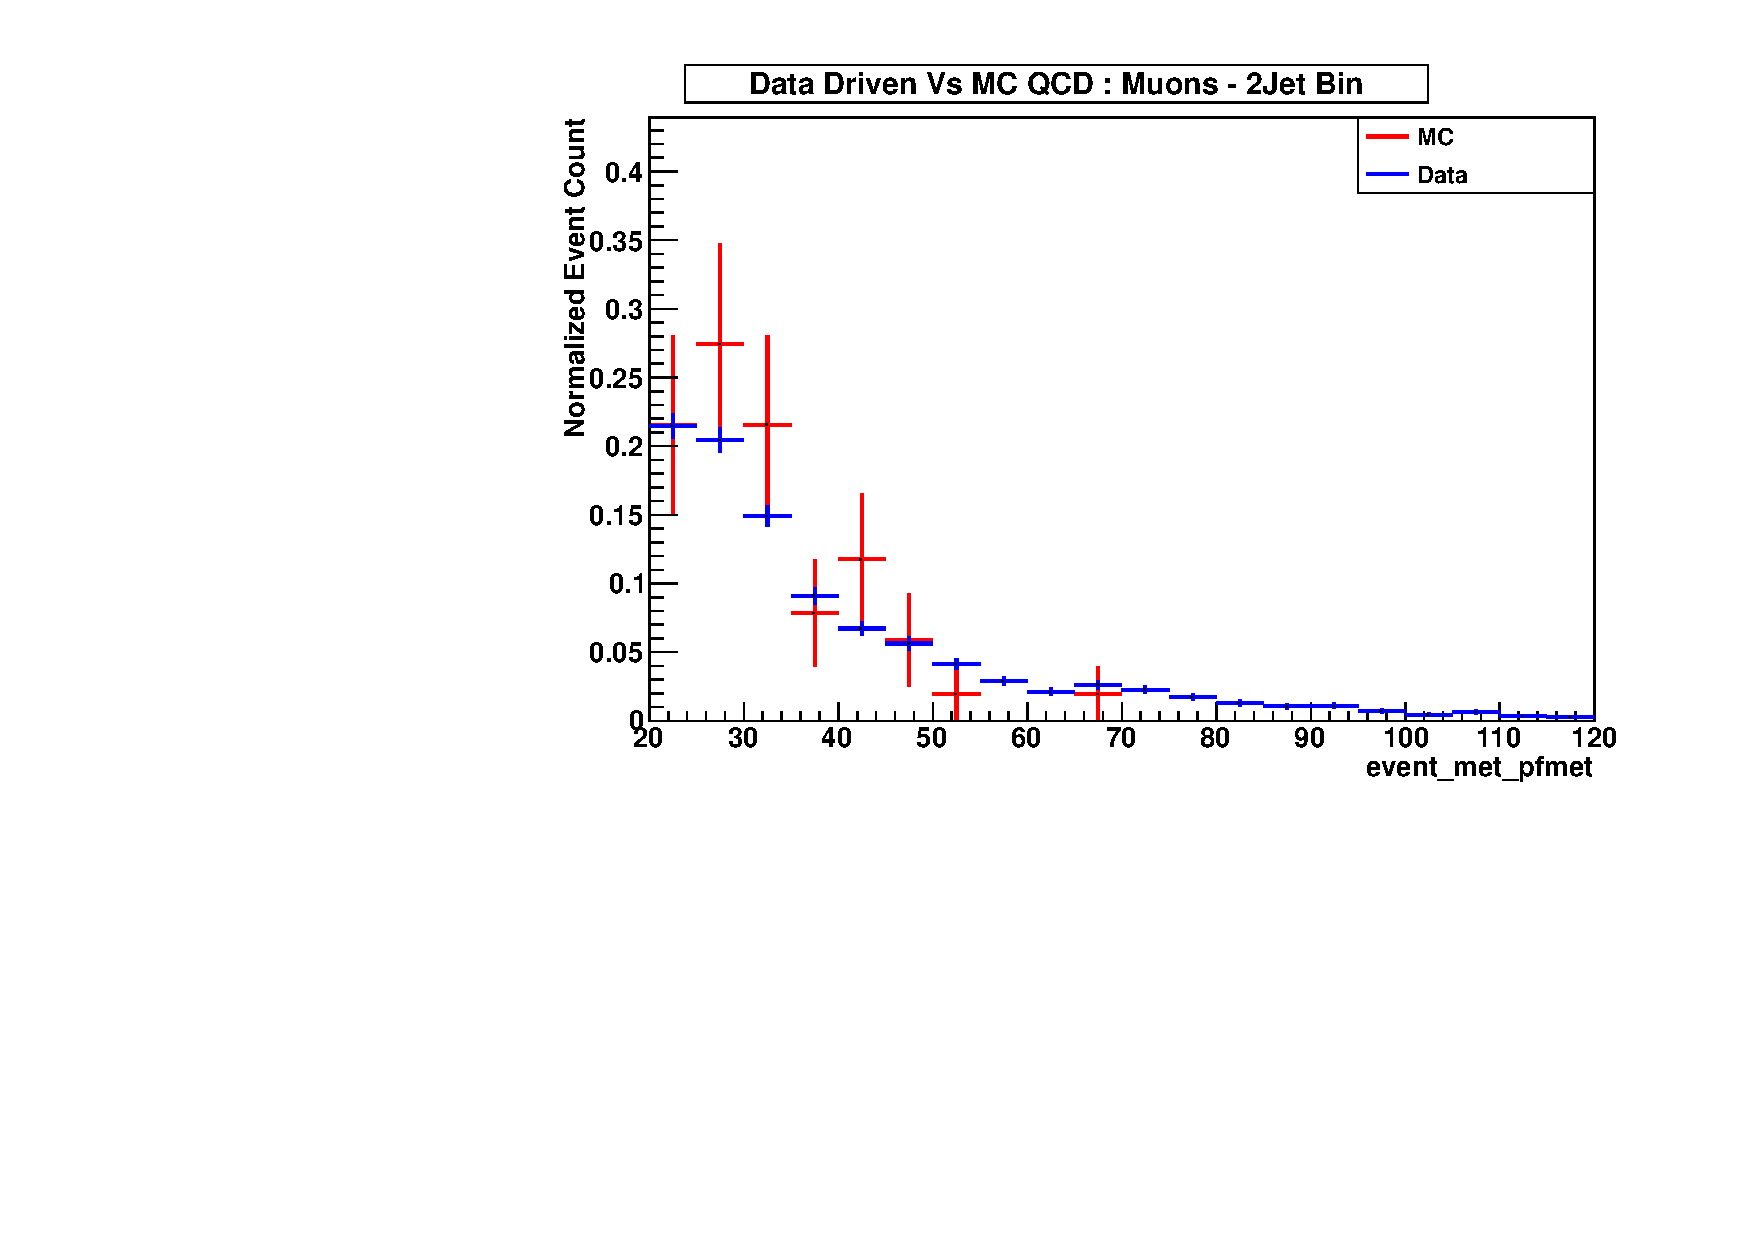
\includegraphics[width=0.48\textwidth]{figs/qcd/QCDDataVSMC_Muons2J_MET.pdf}
\caption{ Comparison of the MET shapes for MC vs data-driven muon QCD events. The two are statistically consistent.} 
\label{fig:QCDCutLoosening_MET}
}
\end{figure}
%%%%%%%
%%%%%%%
\begin{figure}[h!] {\centering
\unitlength=0.33\linewidth
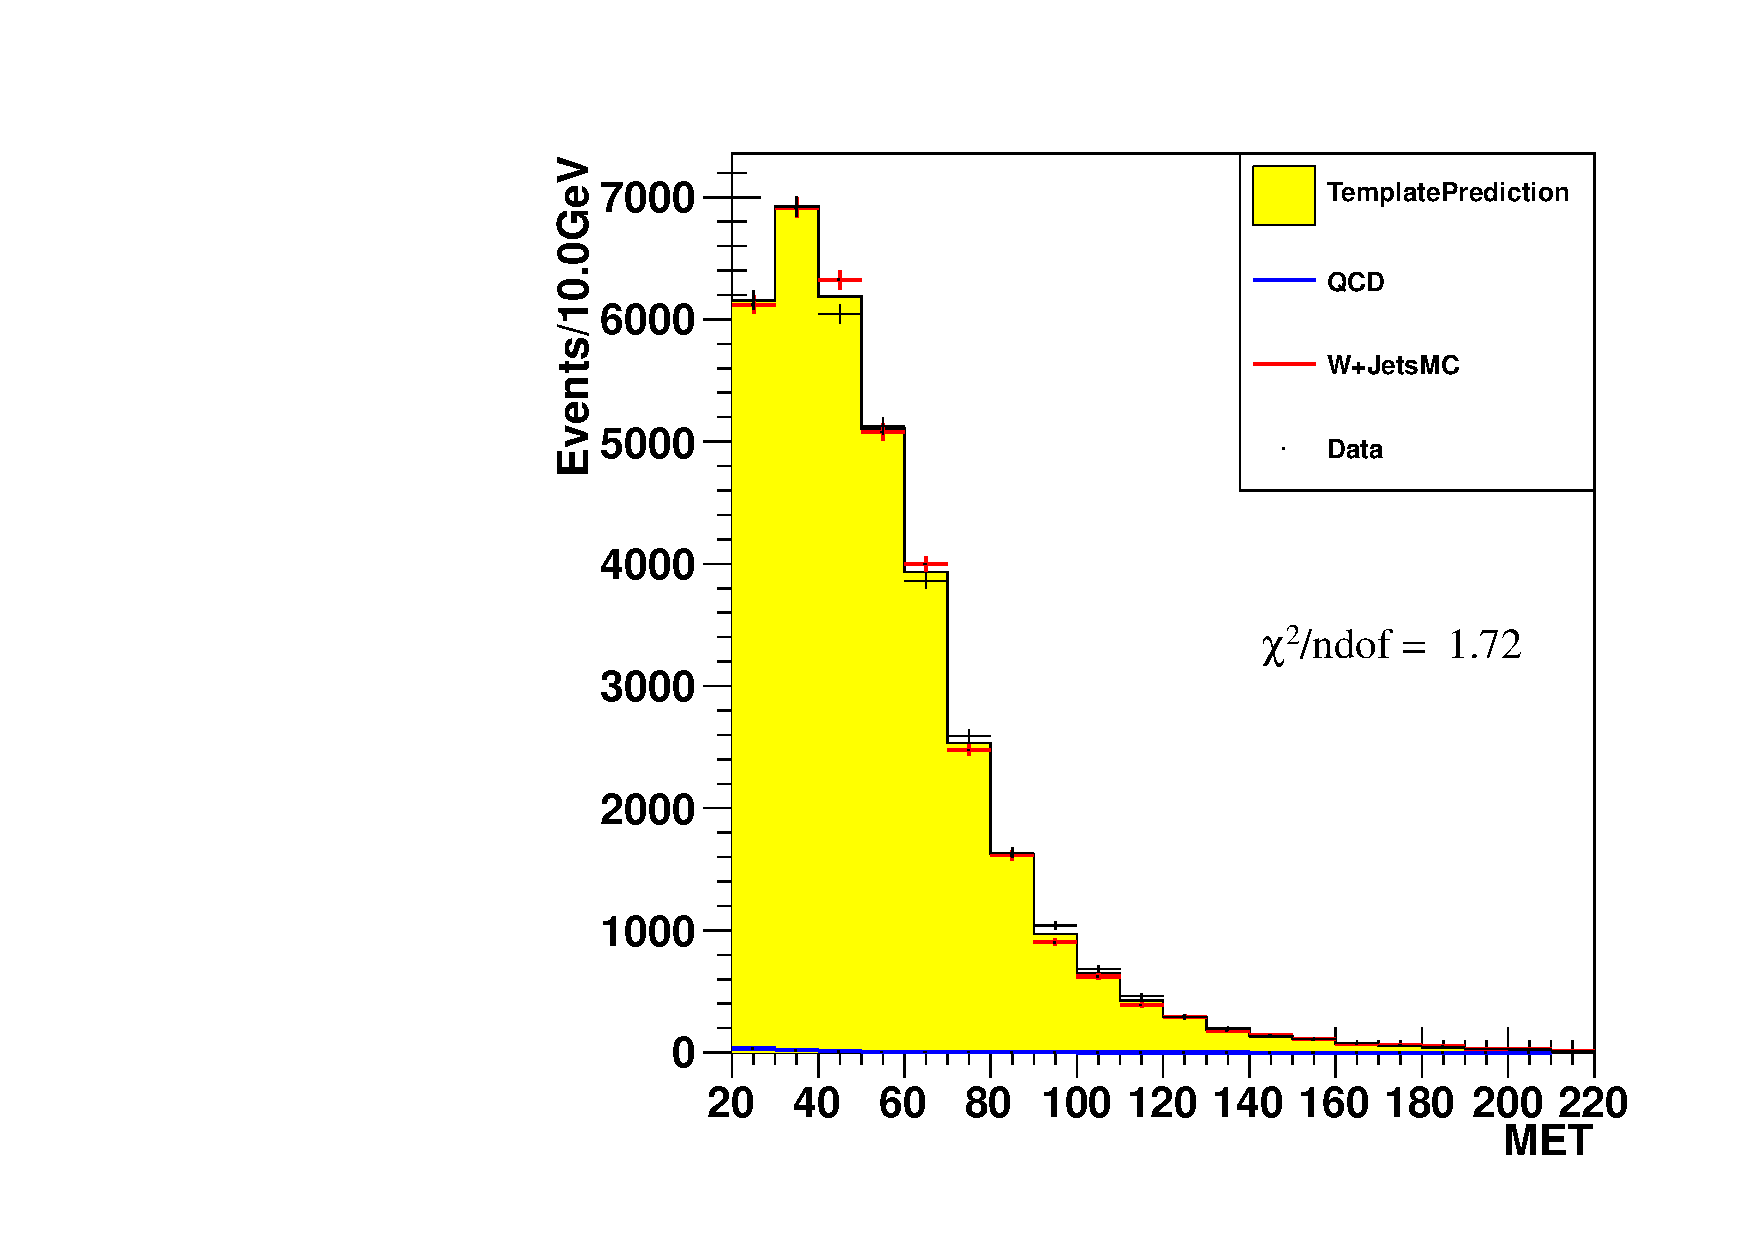
\includegraphics[width=0.48\textwidth]{figs/qcd/TemplateFit_MET_mu2j.pdf}
\put(-0.80,0.0){(a)} 
\unitlength=0.33\linewidth
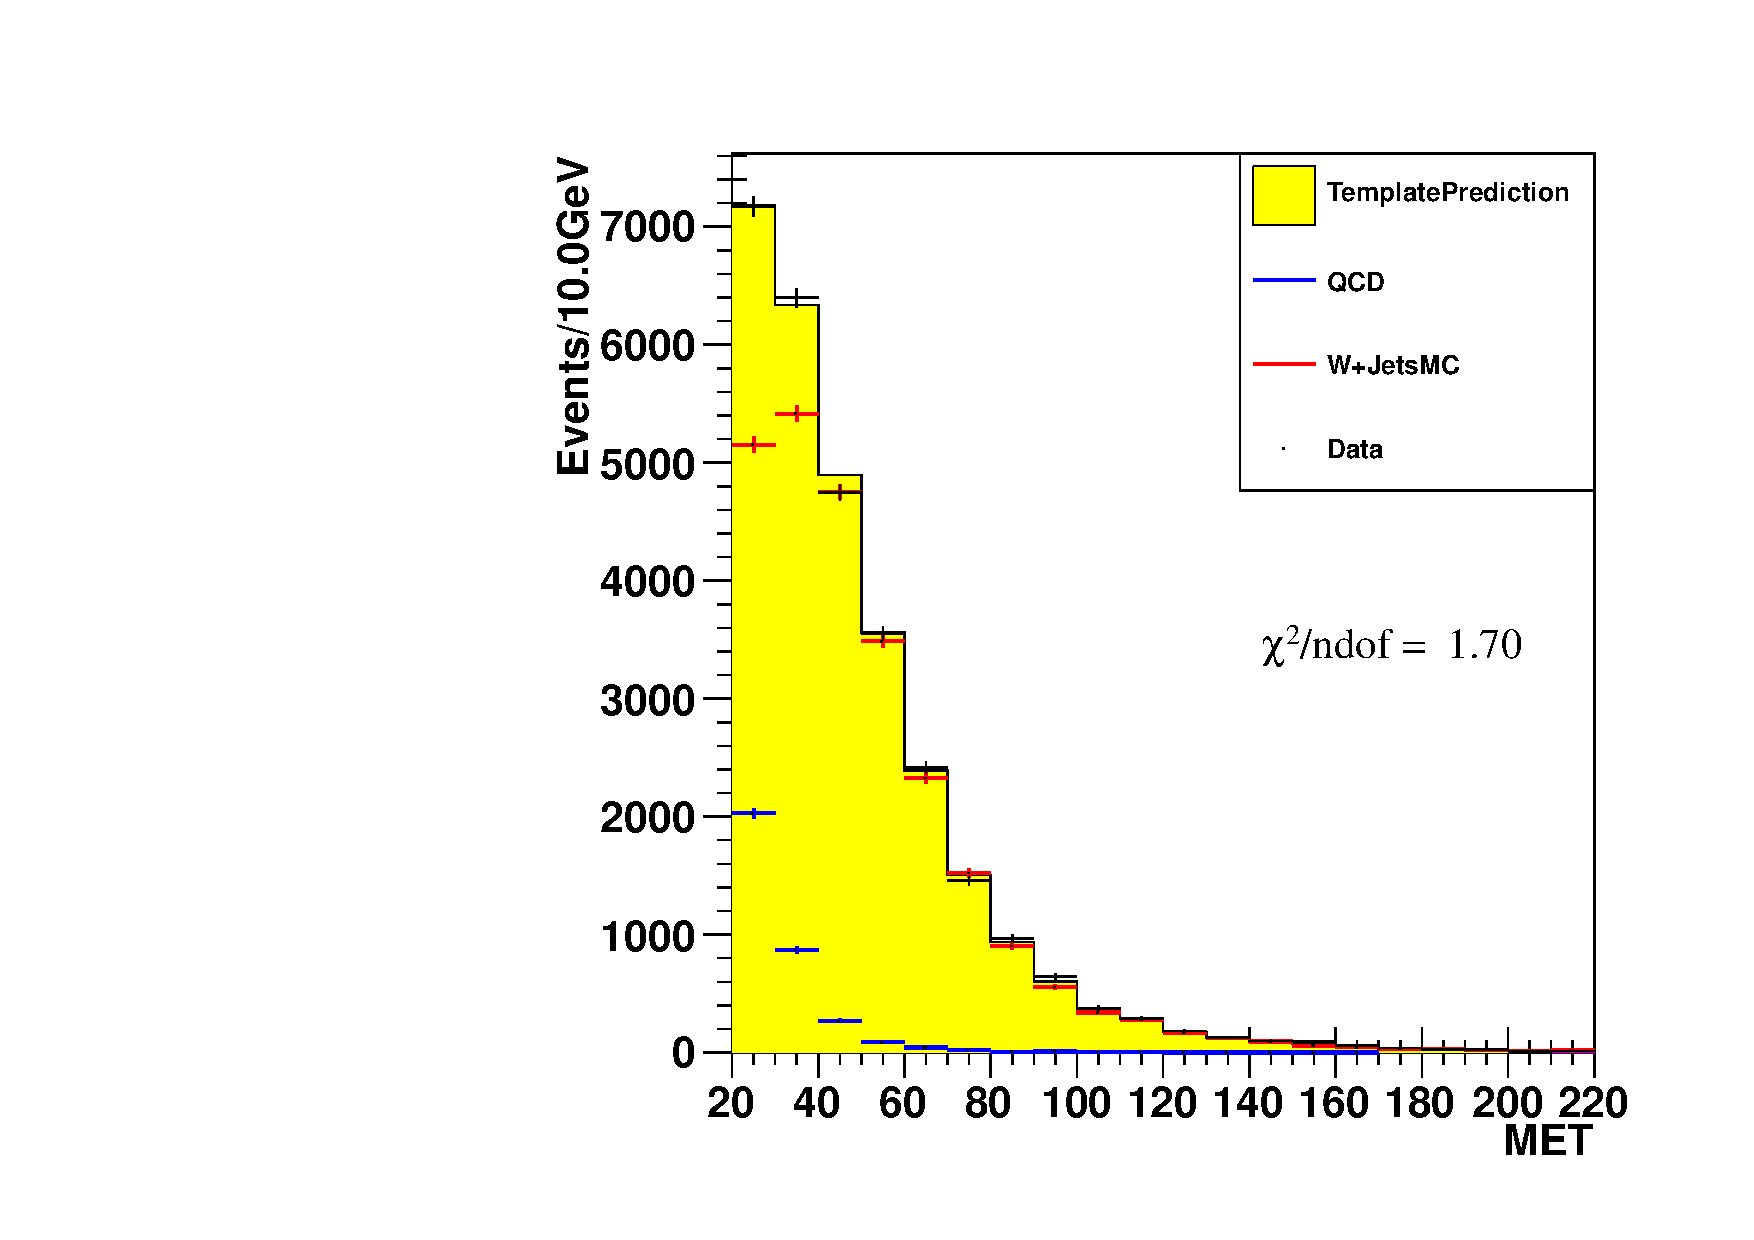
\includegraphics[width=0.48\textwidth]{figs/qcd/TemplateFit_MET_el2j.pdf}
\put(-0.80,0.0){(b)} 
\caption{MET distributions fit to the QCD and W$jj$ templates for: (a) muons, (b) electrons.} 
\label{fig:QCDTemplateFit_MET}
}
\end{figure}
%%%%%%%
%%%%%%%
\begin{figure}[h!] {\centering
\unitlength=0.33\linewidth
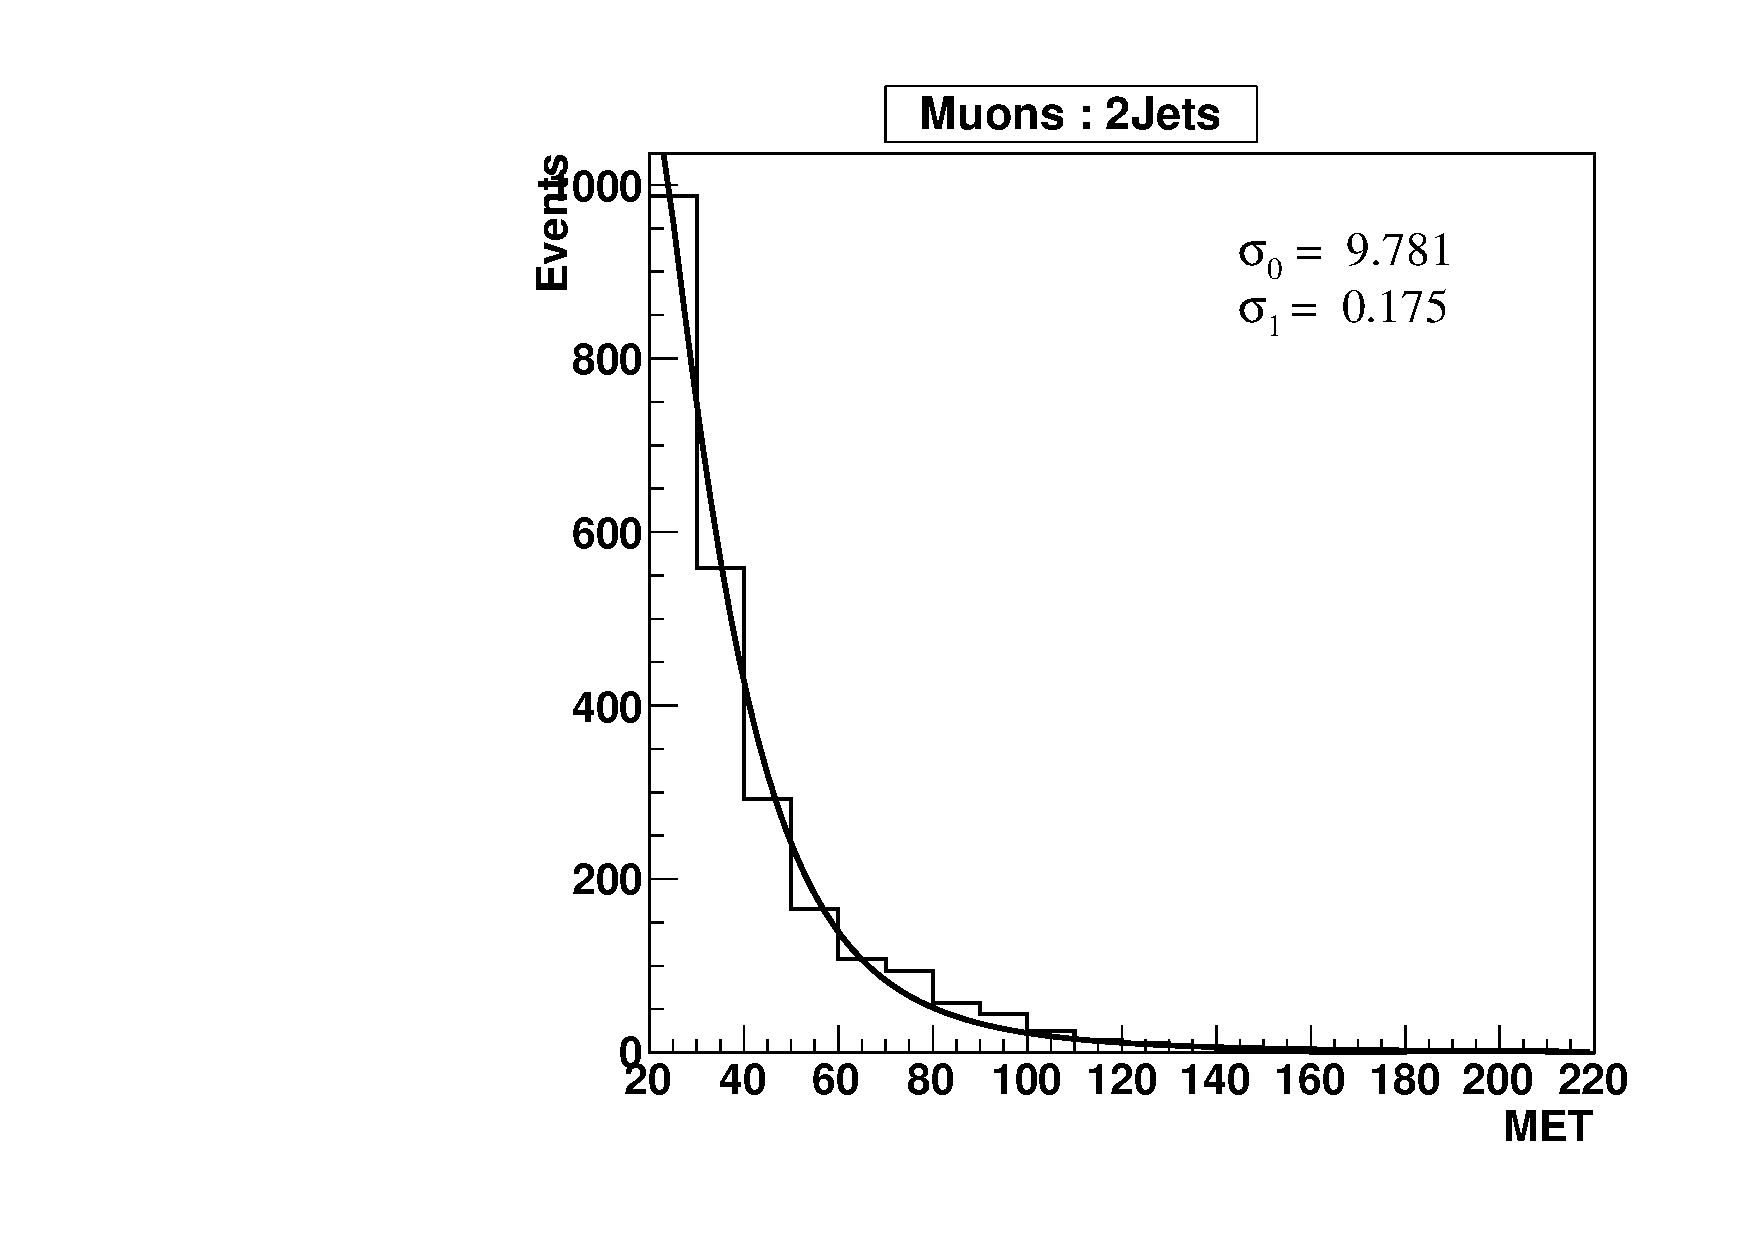
\includegraphics[width=0.48\textwidth]{figs/qcd/RaileighFitQCD_mu2j.pdf}
\put(-0.80,0.0){(a)} 
\unitlength=0.33\linewidth
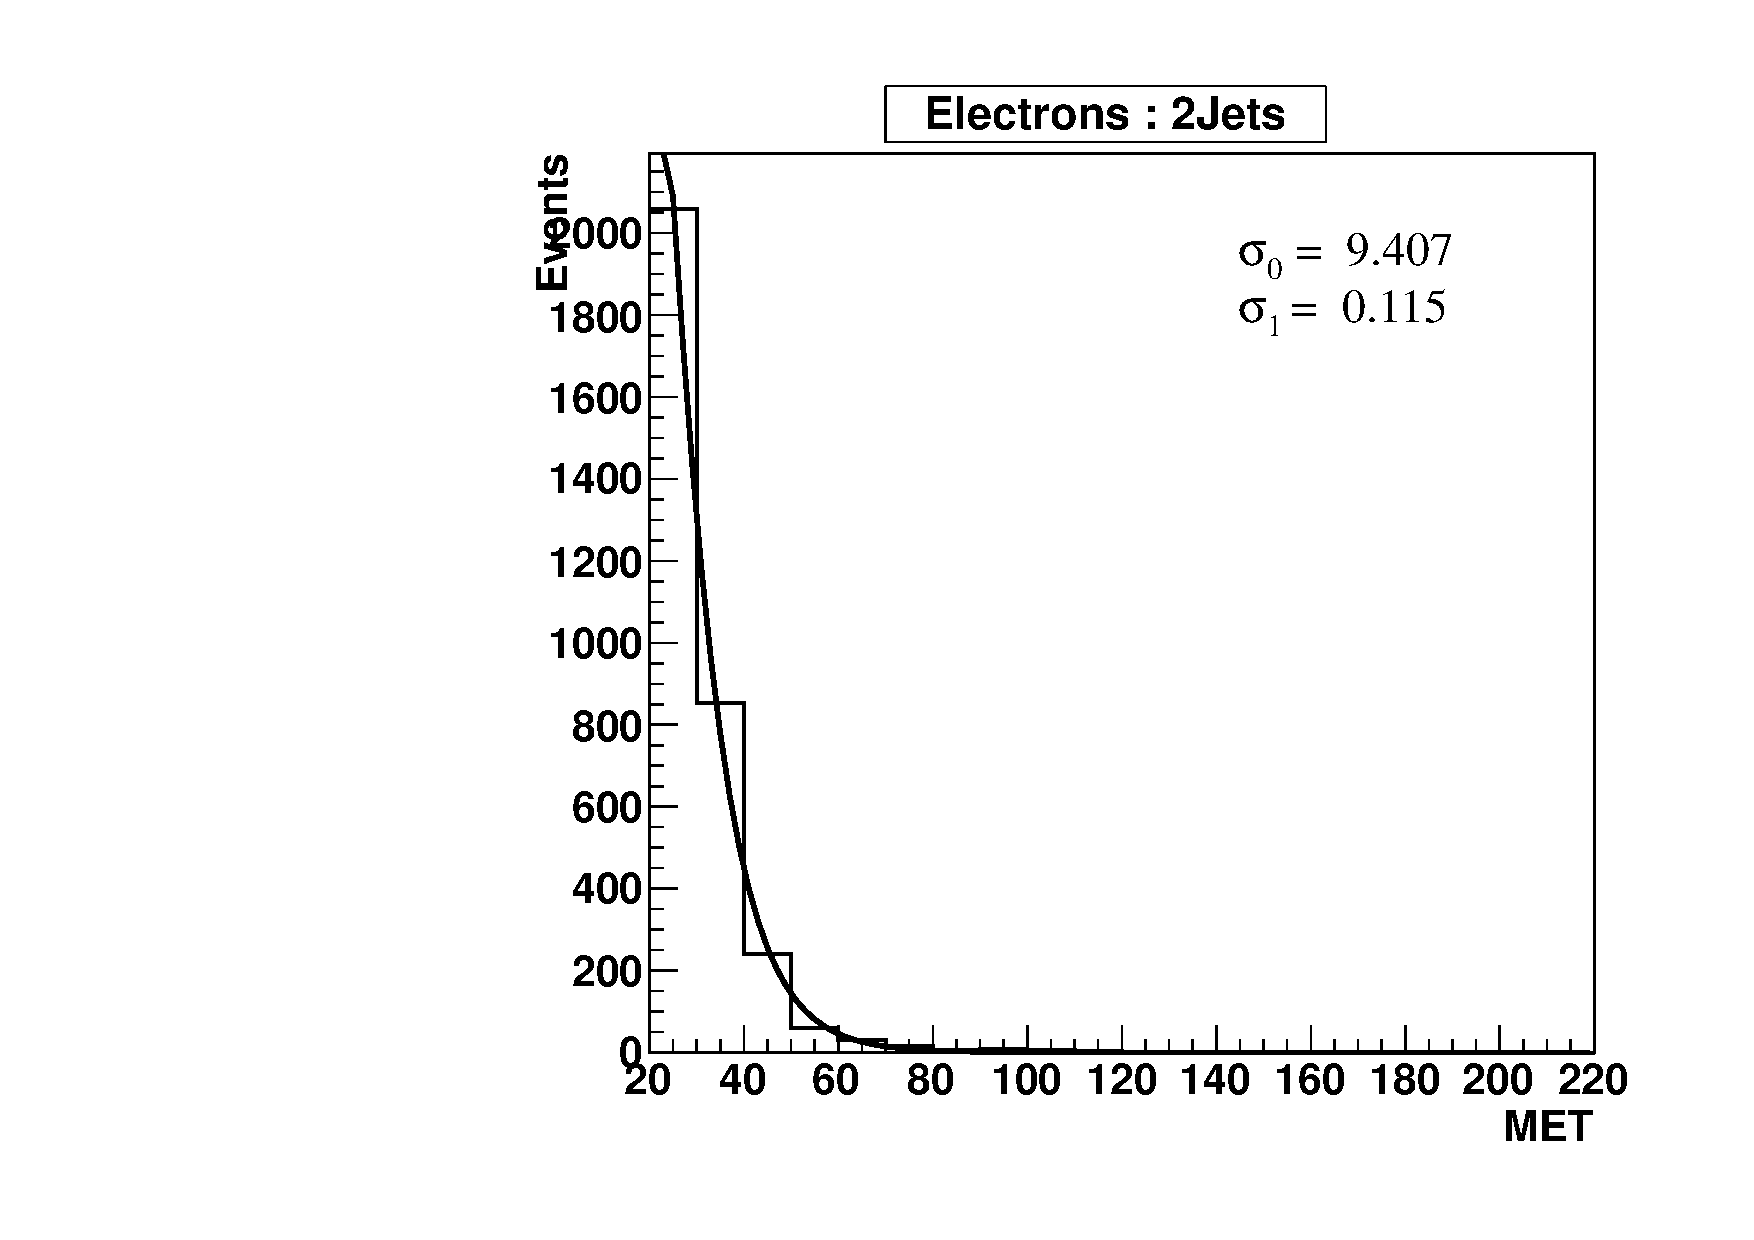
\includegraphics[width=0.48\textwidth]{figs/qcd/RaileighFitQCD_el2j.pdf}
\put(-0.80,0.0){(b)} 
\caption{QCD MET distributions fitted with a Rayleigh Function for: (a) muons, (b) electrons.} 
\label{fig:QCDMETRayleighFit}
}
\end{figure}
%%%%%%%
%%%%%%%
\begin{figure}[h!] {\centering
\unitlength=0.33\linewidth
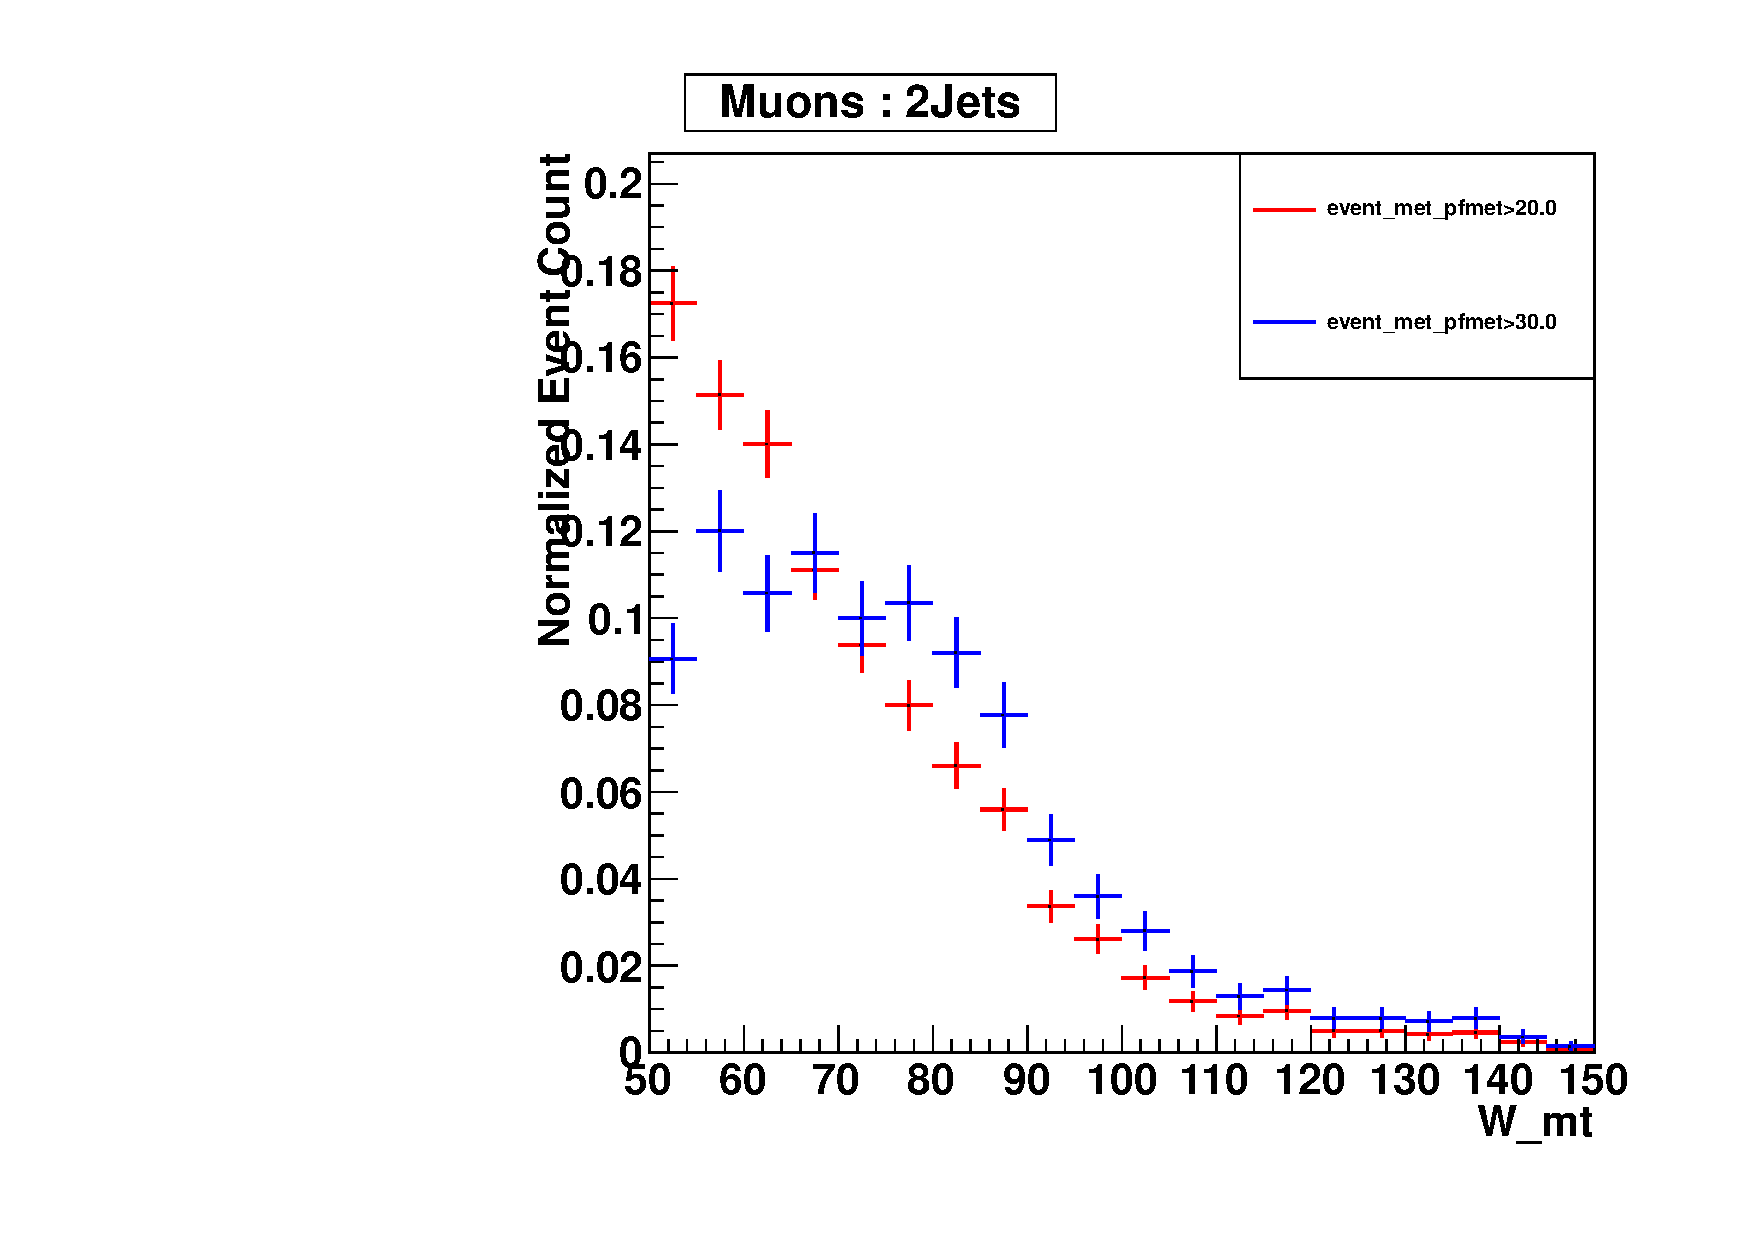
\includegraphics[width=0.48\textwidth]{figs/qcd/METShapeComp_mu2j.pdf}
\put(-0.80,0.0){(a)} 
\unitlength=0.33\linewidth
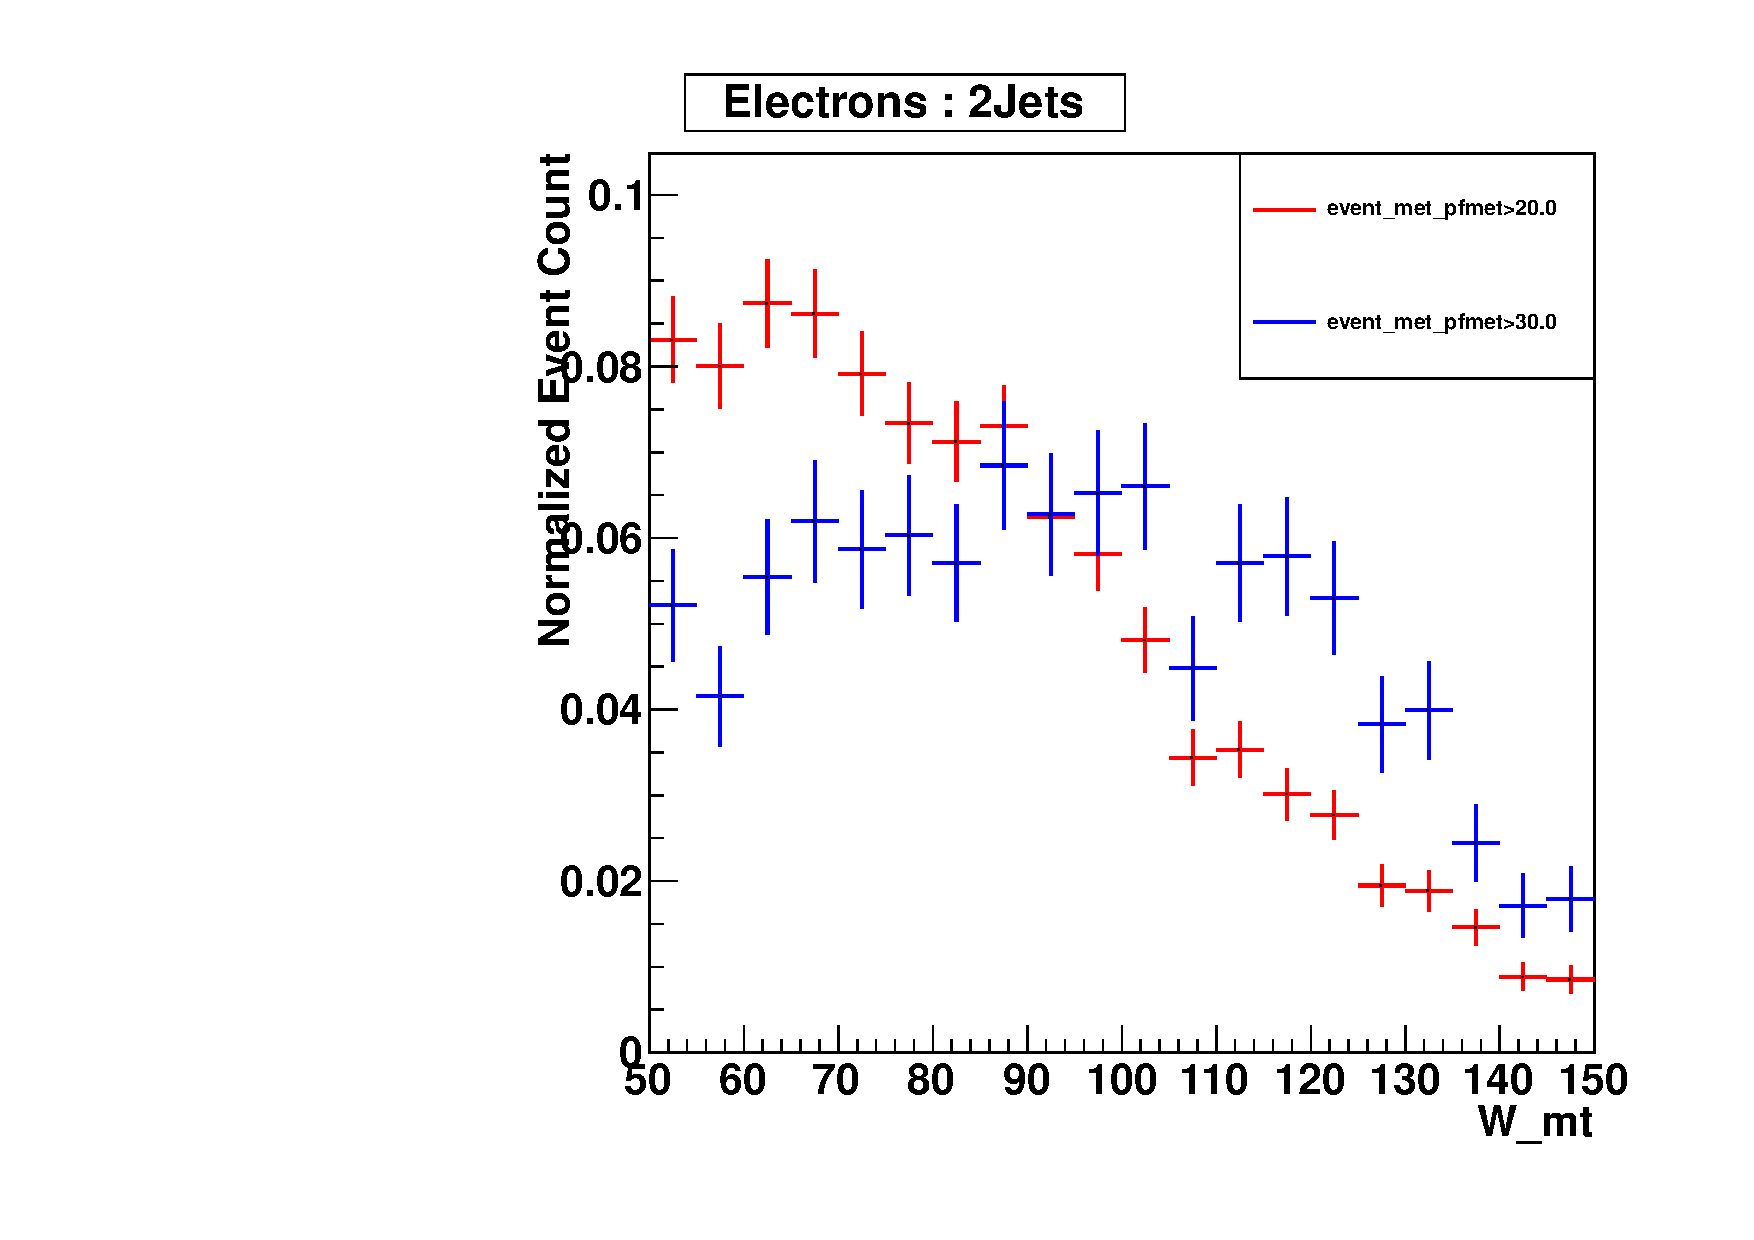
\includegraphics[width=0.48\textwidth]{figs/qcd/METShapeComp_el2j.pdf}
\put(-0.80,0.0){(b)} 
\caption{ QCD W transverse mass shapes with MET$>20$~GeV vs MET$>30$~GeV for: (a) muons, (b) electrons.} 
\label{fig:QCDMETCutsWmTShape}
}
\end{figure}
%%%%%%%
%%%%%%%
\begin{figure}[h!] {\centering
\unitlength=0.33\linewidth
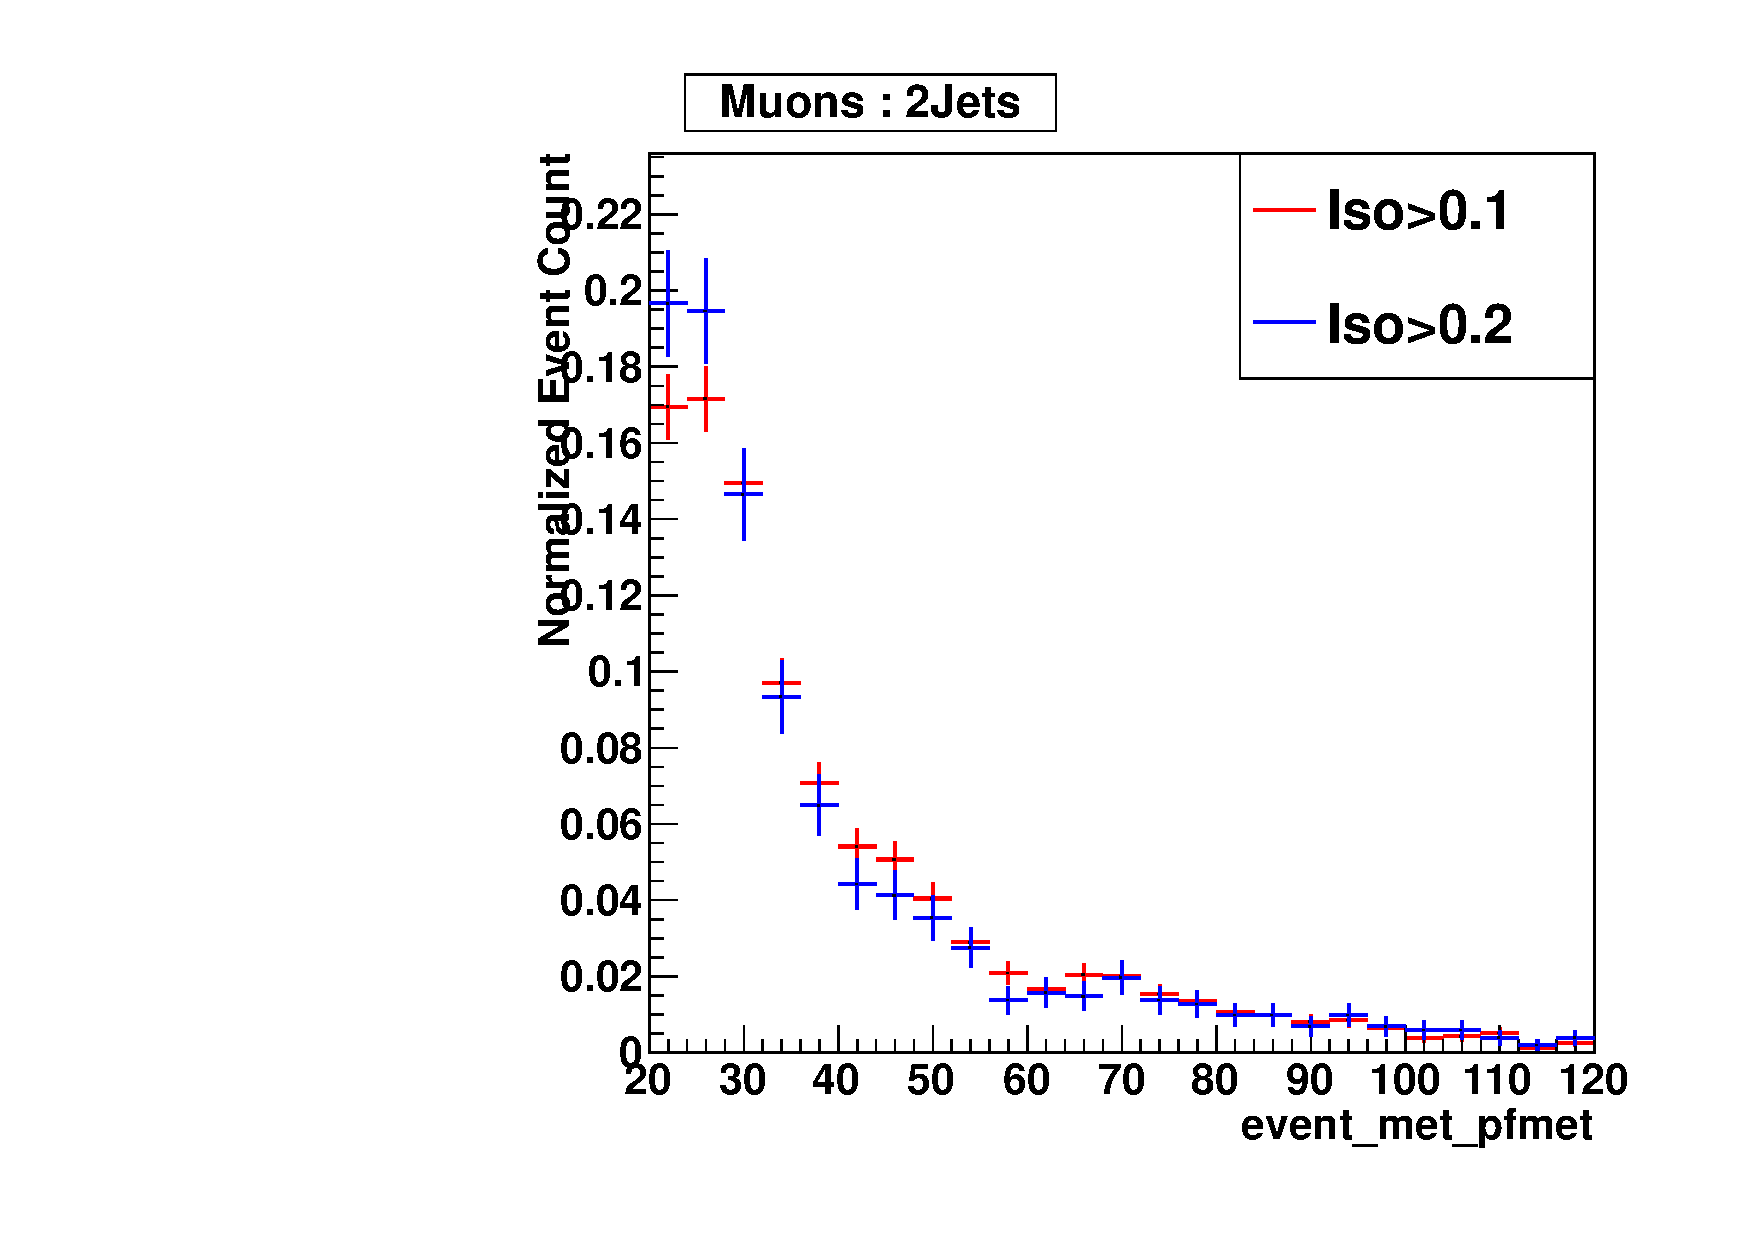
\includegraphics[width=0.48\textwidth]{figs/qcd/ISOShapeComp_MET_mu2j_g01vg02.pdf}
\put(-0.80,0.0){(a)} 
\unitlength=0.33\linewidth
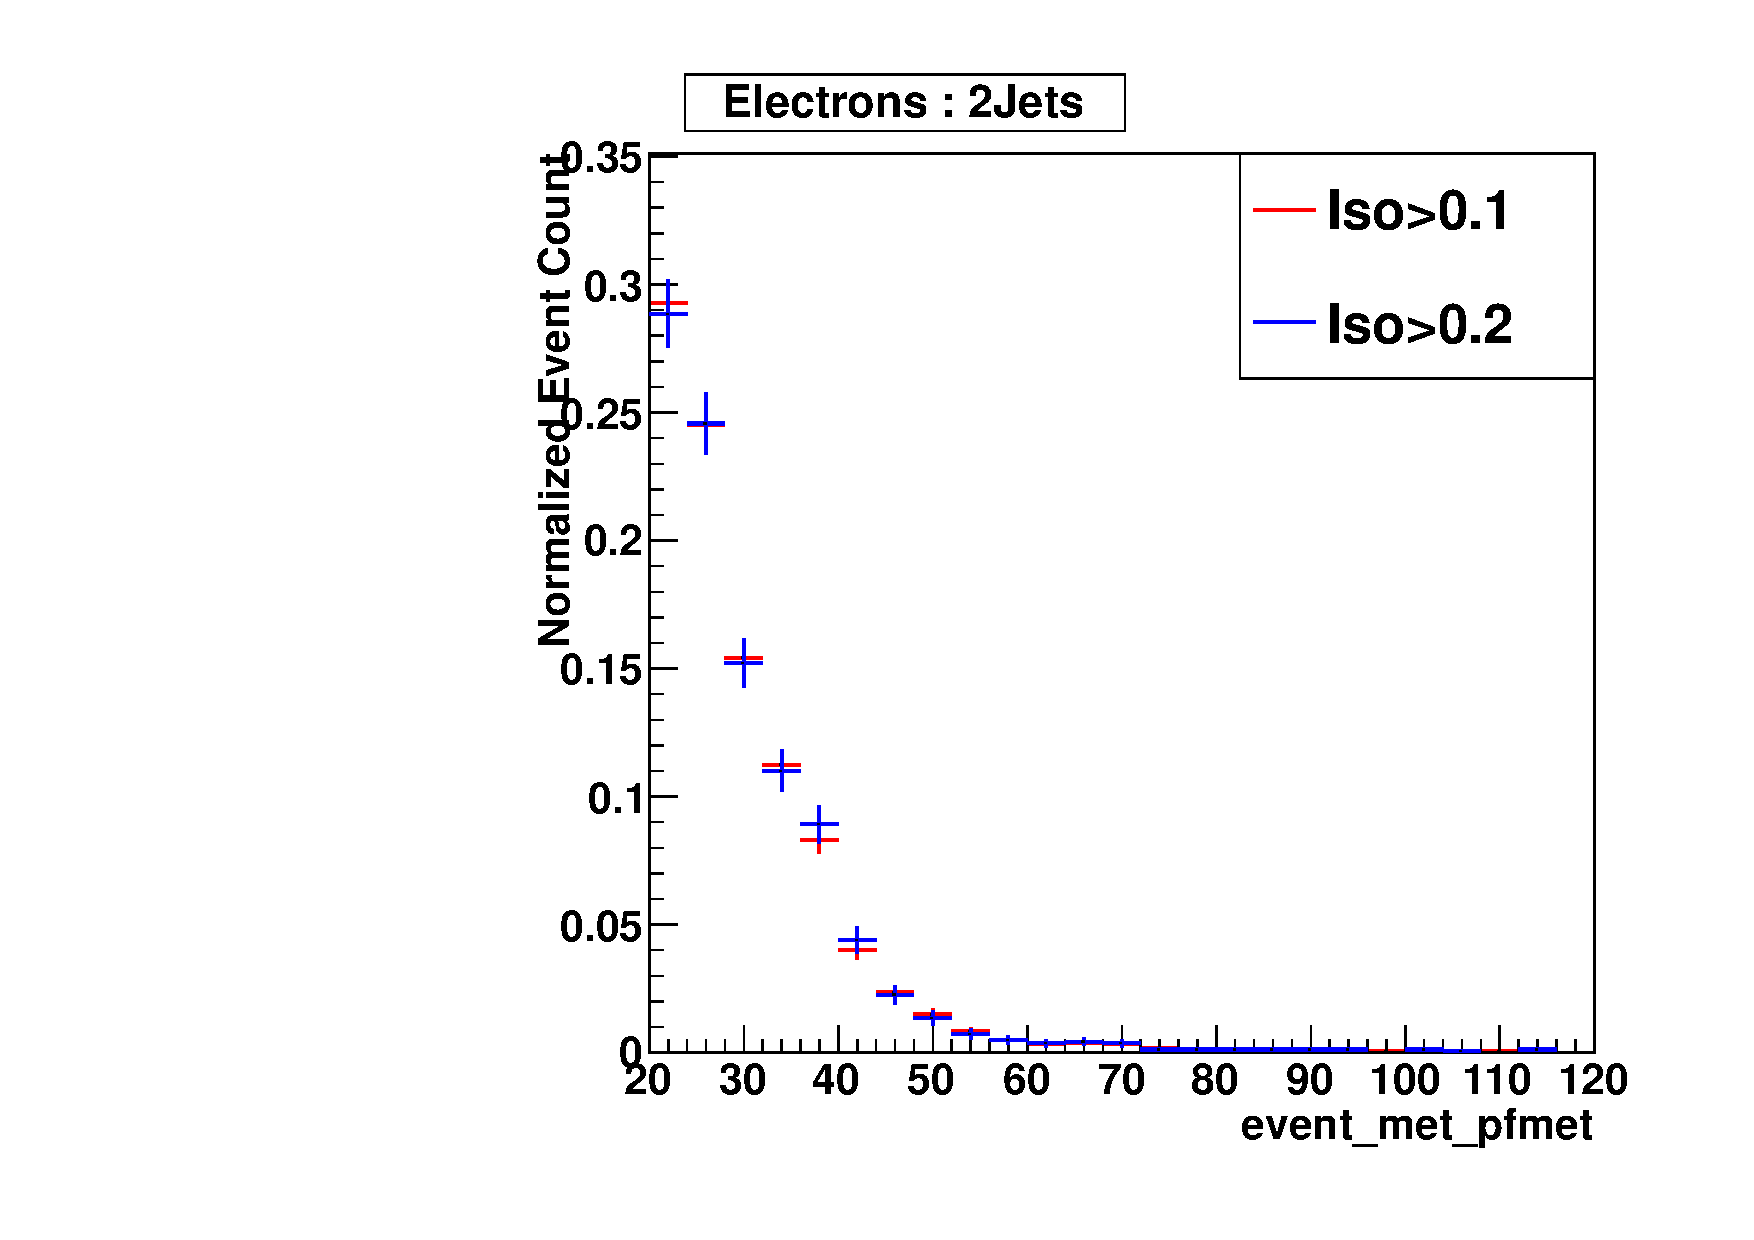
\includegraphics[width=0.48\textwidth]{figs/qcd/ISOShapeComp_MET_el2j_g01vg02.pdf}
\put(-0.80,0.0){(b)} 
\caption{ QCD MET shapes with Iso$>0.1$ vs Iso$>0.2$ for: (a) muons, (b) electrons.} 
\label{fig:QCDISOCutsMETShape}
}
\end{figure}
%%%%%%%
%%%%%%%
\begin{figure}[h!] {\centering
\unitlength=0.33\linewidth
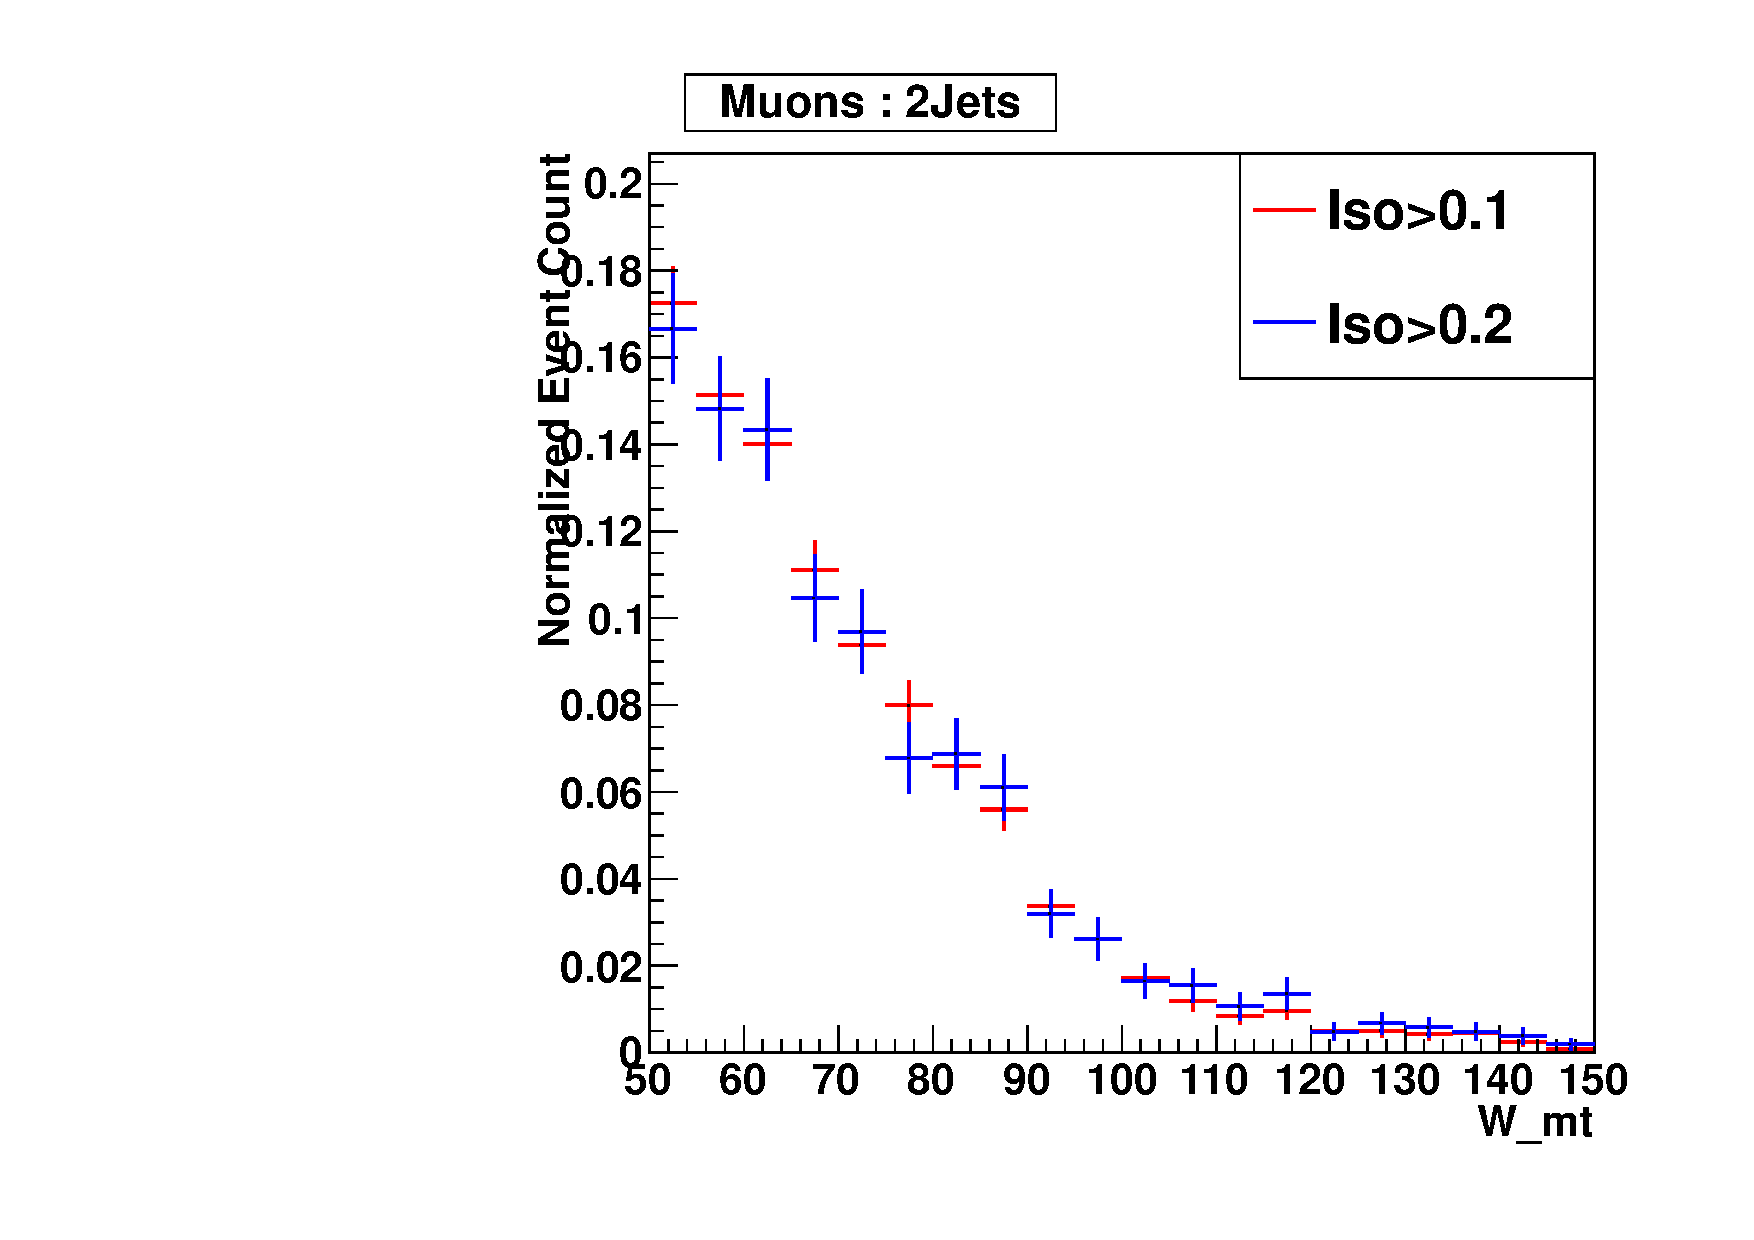
\includegraphics[width=0.48\textwidth]{figs/qcd/ISOShapeComp_WmT_mu2j_g01vg02.pdf}
\put(-0.80,0.0){(a)} 
\unitlength=0.33\linewidth
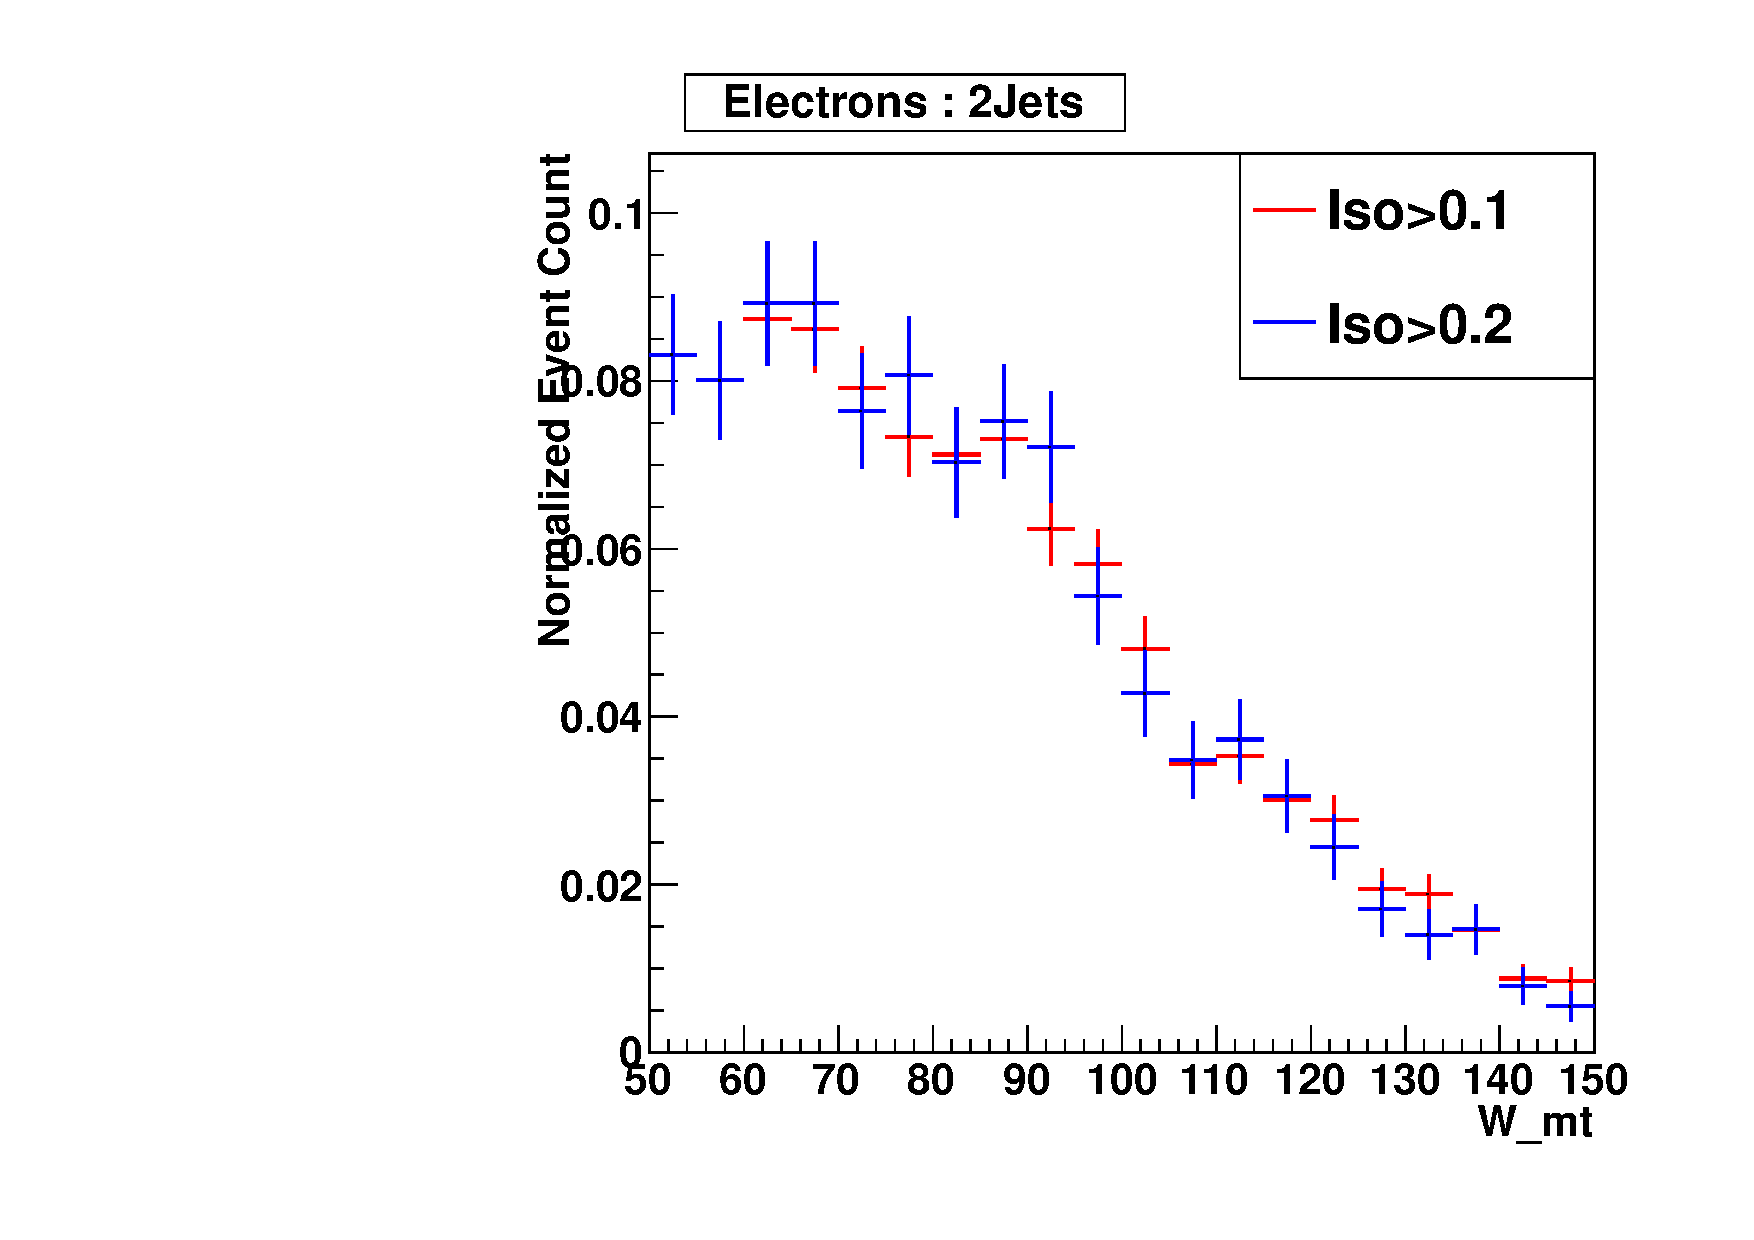
\includegraphics[width=0.48\textwidth]{figs/qcd/ISOShapeComp_WmT_el2j_g01vg02.pdf}
\put(-0.80,0.0){(b)} 
\caption{ QCD W transverse mass shapes with Iso$>0.1$ vs Iso$>0.2$ for: (a) muons, (b) electrons.} 
\label{fig:QCDISOCutsWmTShape}
}
\end{figure}

%%%%%%%%%%%%%%%%%%%%%%%%%%%%%%%%%
\subsection{Effect of pileup and inflation of QCD uncertainty}
In order to be able to get a pure QCD control sample we needed to invert 
the lepton isolation. 
However, the single lepton triggers were loose enough to allow 
sufficient statistics of QCD events only in the first  200~\invpb of 2011A data.
After that the single lepton triggers used isolation and tight ID requirements 
in the HLT.
Thus, we effectively use a sample of events based on 200~\invpb data  
and extrapolate the QCD shape to the full data sample.  
Since the pileup conditions were more severe in the bulk of the data 
we need to consider any systematic uncertainty that might occur from this extrapolation. 
The ideal way to deal with this would be to compare subsets of the
data or QCD MCs with different pileup conditions. 
However, there is not enough statistics of QCD events to get precise shape 
even in the full data and MC samples (the latter corresponds to only $O(10-100)$~\invnb.
This is one of the reasons that we inflate the QCD uncertainty to 50\% 
for electron data and 100\% (or larger) for muon data.
%%%%%%%%%%%%%%%%%%%%%%%%%%%%%%%%%%%%%%%%%%%%%%%%%%%%%%%%%%%%%%%%%%
%%%%%%%%%%%%%%%%%%%%%%%%%%%%%%%%%%%%%%%%%%%%%%%%%%%%%%%%%%%%%%%%%%
%%%%%%%%%%%%%%%%%%%%%%%%%%%%%%%%%%%%%%%%%%%%%%%%%%%%%%%%%%%%%%%%%%
%%%%%%%%%%%%%%%%%%%%%%%%%%%%%%%%%%%%%%%%%%%%%%%%%%%%%%%%%%%%%%%%%%

\clearpage
\section{W+jets shape}
\label{sec:wjetsShape}

In order to get a good description of the W+jets shape in data, the
simulation needs to describe well both the matrix elements for the
hard processes, and the subsequent development of the hard partons
into jets of hadrons.  However, no factorization theorem exists to
rigorously separate these two components.  A given (n + 1)-jet event
can be obtained in two ways: from the collinear/soft-radiation
evolution of an appropriate (n + 1)-parton final state, or from an
n-parton configuration where hard, large-angle emission during its
evolution leads to the extra jet.  A factorization scheme defines, on
an event-by-event basis, which of the two paths should be followed.
The two relevant parameters defining such a scheme are: the
factorization/renormalization scale $q^2$ and the matrix element -
parton shower matching threshold.  Optimized values of these
parameters should give the best possible approximation to the W+jets
kinematics for a given fixed-order calculation.  We know that the
physics has to be independent of the relative contributions of the two
components.

The CMS MadGraph W+jets production uses MLM matching
\cite{Hoche:2006ph} with $k_T$ jets.  The default matching threshold
is 20~GeV (i.e., if the parton $p_{T}$ is greater than 20~GeV, then it
is assumed to have originated from the hard scattering process and
contributes to the matrix element calculation; if the parton $p_{T}$
is less than 20~GeV then it is assumed to come from the parton
shower).  The factorization/renormalization scale $q^2$ corresponds to
the ``transverse mass'' of the W boson: $\sqrt{M_W^2 + p_{T, W}^2}$.

\subsection{Factorization/renormalization scale and matrix element - parton shower matching threshold}
\label{sec:wjetsShapeMatchingQ2}

To perform studies of the uncertainty due to the choice of the $q^2$
and matching scales, alternative MadGraph W+jets samples are produced
in which the corresponding scales are changed by a factor of 2.  Thus,
we have ``matching-up'', ``matching-down'', ``scale-up'', and
``scale-down'' samples, each yielding an $m_{jj}$ distribution, or
template.  %Our use of these templates is shown schematically in
%Fig.~\ref{fig:mjj2body} and described below.
%Figure~\ref{fig:wjetshapes} shows the input MC $m_{jj}$ templates that
%are we have availible.

We can use our samples to find an optimum MC template
$\mathcal{F}_{W+\text{jets}}$,
%%\[
\begin{equation}
\mathcal{F}_{W+\text{jets}} = \sum_\alpha f_\alpha \mathcal{G}_\alpha\, + (1-\sum_\alpha f_\alpha)\times\mathcal{G}_\text{nominal},
\label{eqn:wjetsShapeMatchingQ2}
\end{equation}
%%\]
where $\alpha \in
\{\text{matchingUp,matchingDown,scaleUp,scaleDown}\}$,
$\mathcal{G}_\text{nominal}$ is the template from the default MadGraph
generation and $\mathcal{G}_\alpha$ is the template from the specified
sample.  We define a 2D coordinate system in scale and matching.  The
origin corresponds to the default MadGraph sample.  To move in the
positive scaleUp direction, one sets $f_\text{scaleDown}=0$ and
increases $f_\text{scaleUp}$. To move in the negative scaleUp
direction, one sets $f_\text{scaleUp}=0$ and increases
$f_\text{scaleDown}$.  The same is true for the matching samples.  We
allow the relative contributions from these templates to float in our
fit.  This lets the data determine the best W+jets shape and the
uncertainties on these parameters is automatically propagated to the
uncertainties on the yields.

Because of the b-tagging selection cuts used we take the approach of
parameterizing the W+jets background contribution for the events with
at least one btag.  We use the default MadGraph samples, weighted
appropriately for trigger efficiency and other known effects, as a
starting place for determining the shape of the background.  We find
that given our selection we can well model the background shape of the
W+jets component using a sum of a Gaussian distribution and an
exponential shape.  The result of an unbinned maximum likelihood fit
to the MC distributions is shown if Fig.~\ref{fig:WpJFit}.  As can be
seen the agreement with the projection is good.  The electrons are fit
using only a Gaussian shape as this is sufficient.

\begin{figure}
\begin{center}
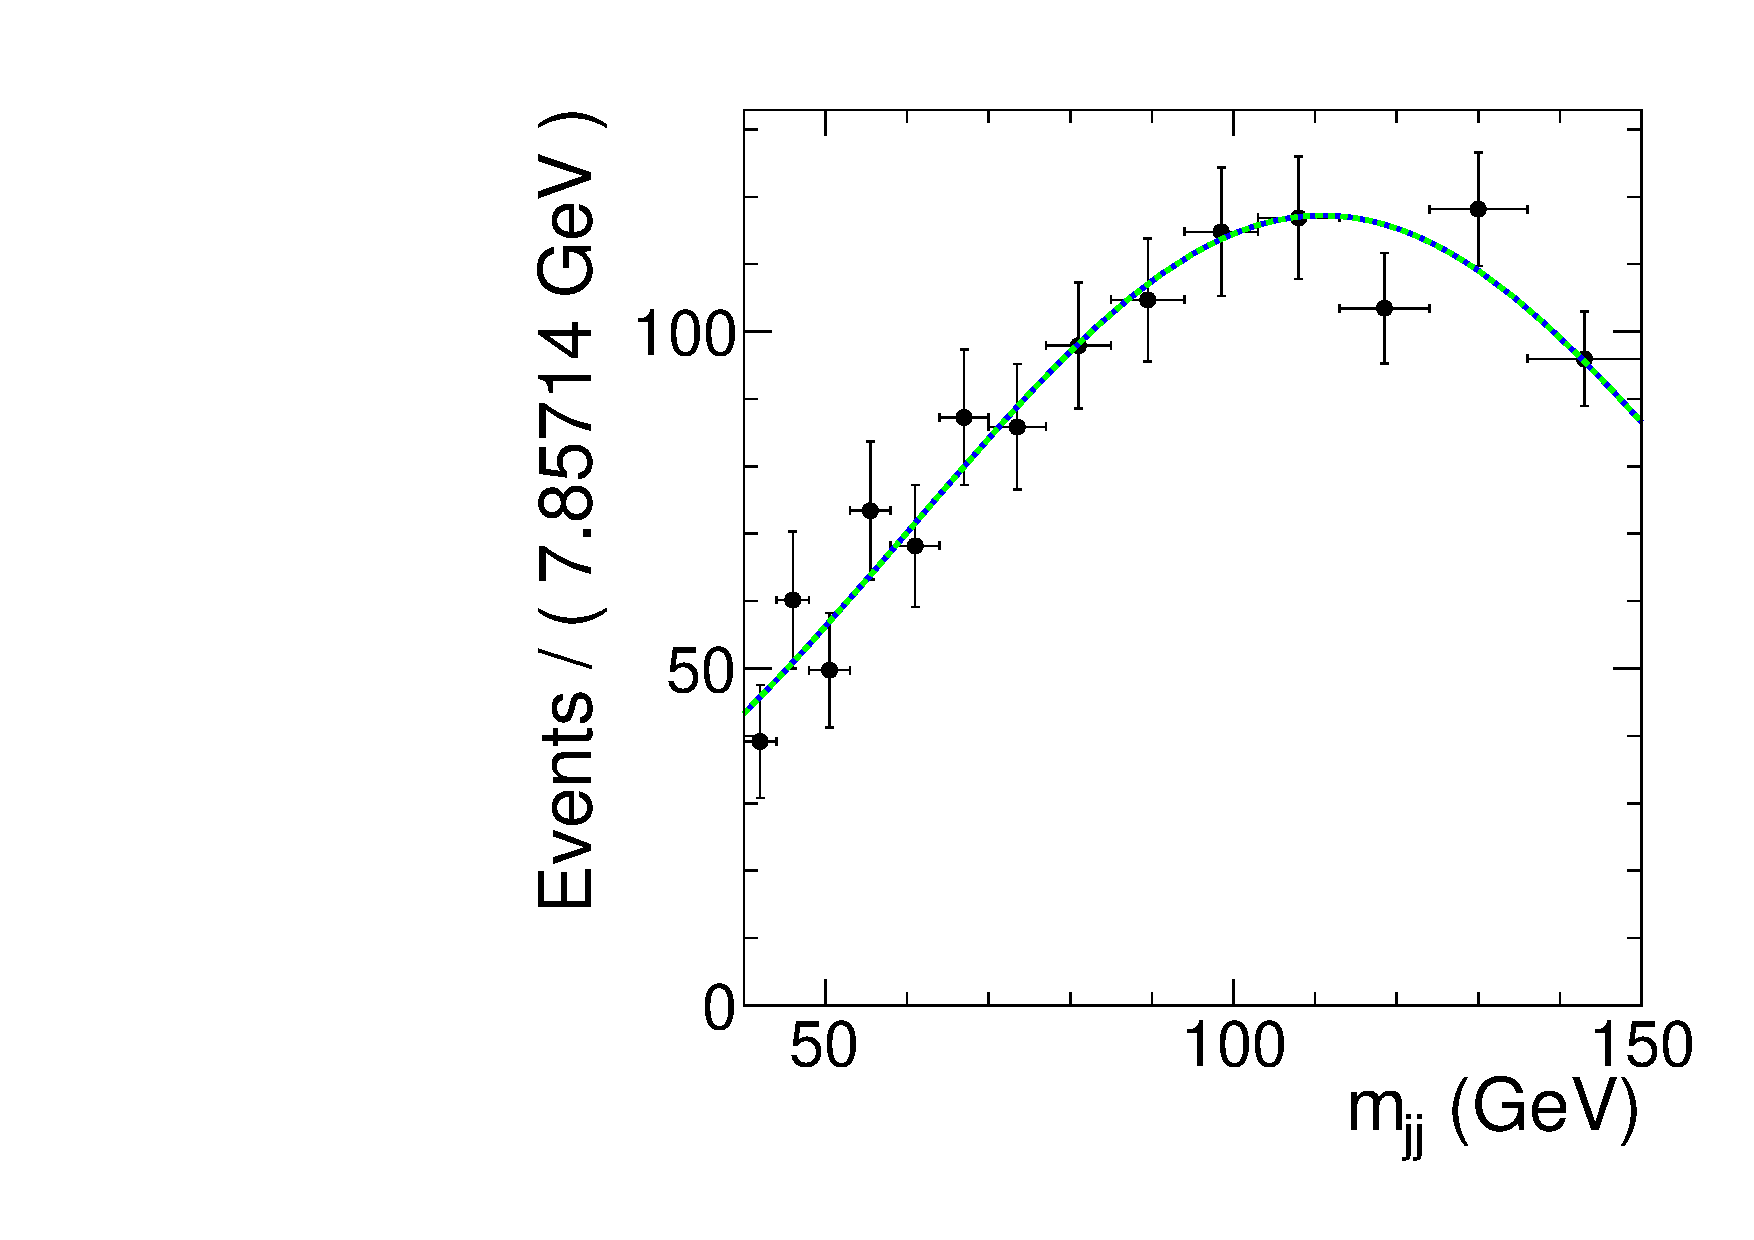
\includegraphics[width=0.45\textwidth]{figs/wpj/WpJShape_Diboson_electrons_btagged}
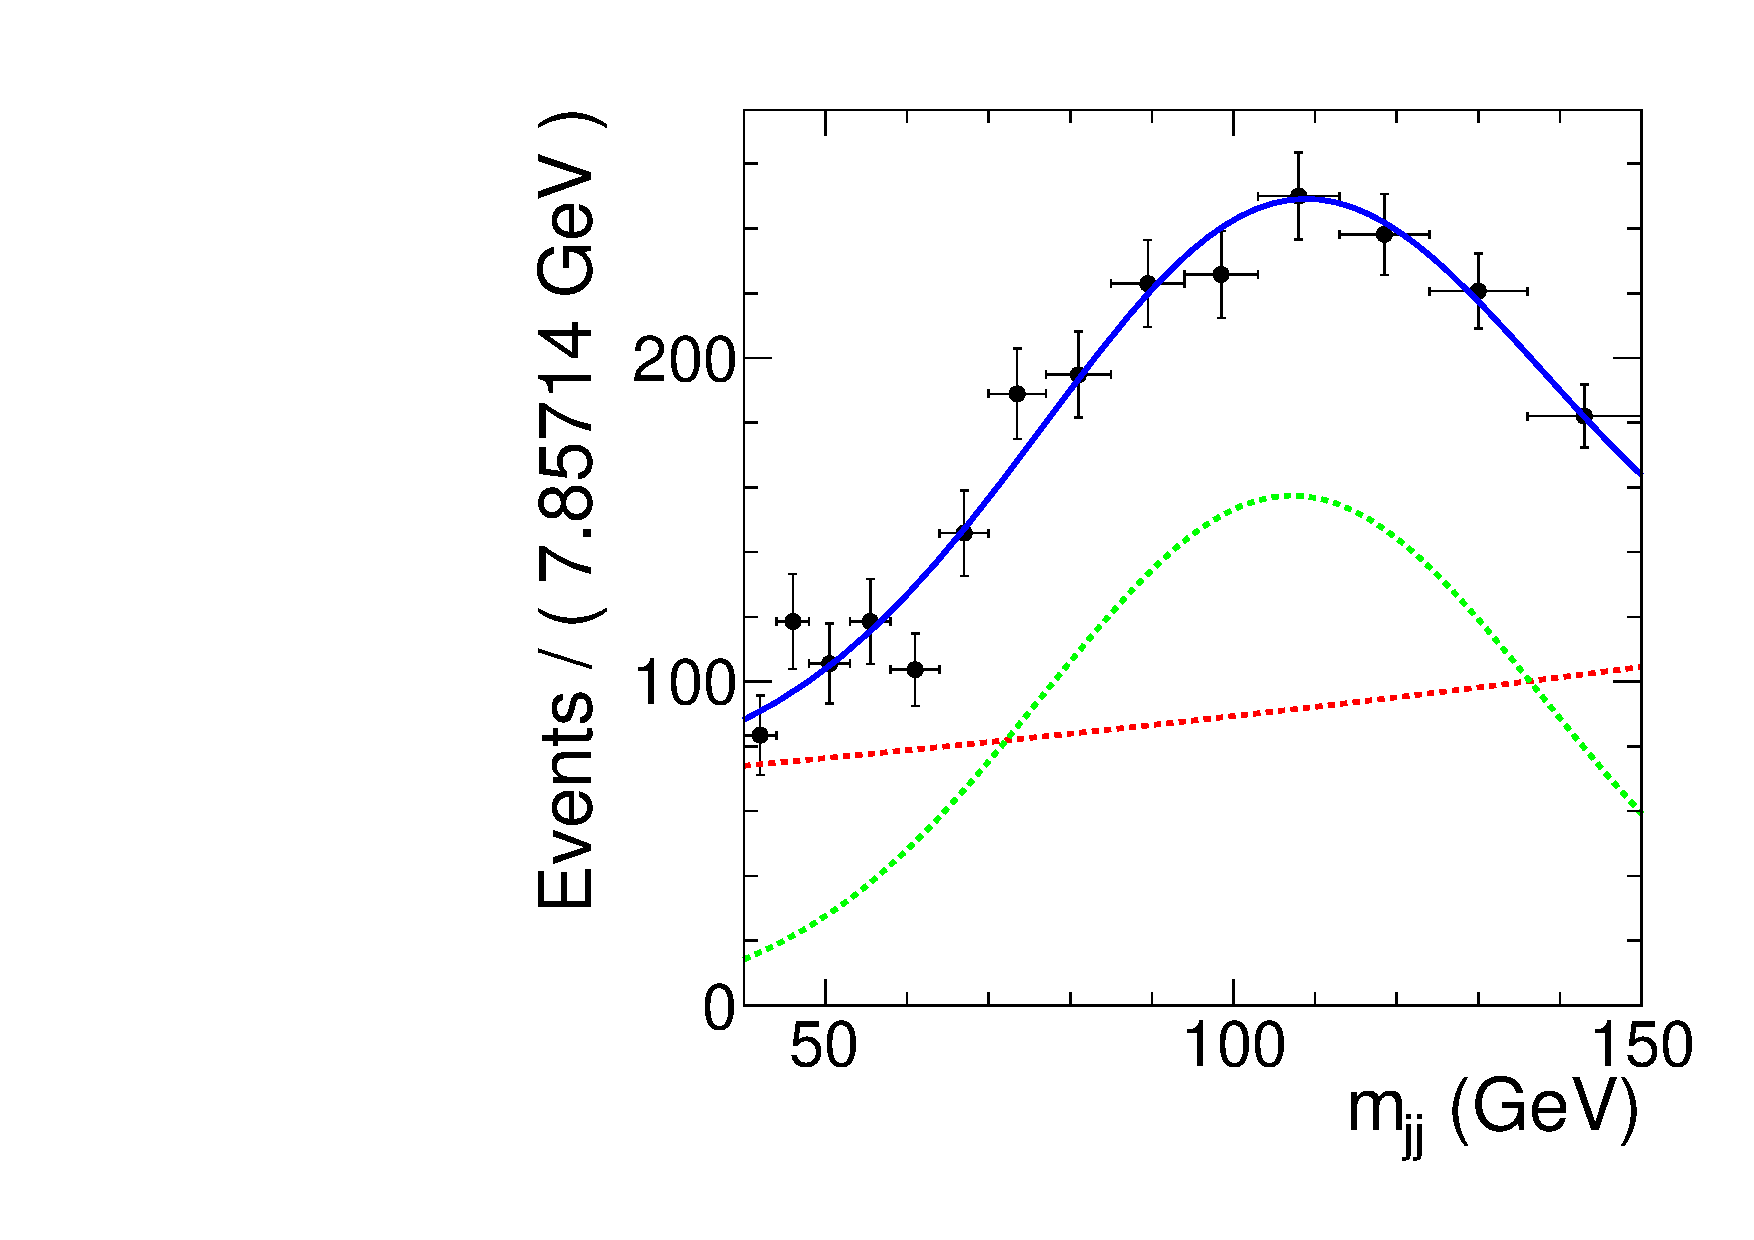
\includegraphics[width=0.45\textwidth]{figs/wpj/WpJShape_Diboson_muons_btagged}
\end{center}
\caption{\label{fig:WpJFit} W+jets shape in the b-tagged sample:
Projection of a fit to the W+jets MC with our
proposed parameterization for electrons (left) and muons (right).  The
components of the parameterization are shown as well as their sum.}
\end{figure}

The W+jets MC availible for this analysis corresponds to less than the
amount of integrated luminosity.  We take the values from the fit to
the MC as a starting place for the data fit.  We apply Gaussian
constraints on the parameters equal to the statistical error from the
MC fit.  This allows the shape of the W+jets component of the
background some limited freedom to adapt to likely differences between
data and MC.

\section{Diboson signal shape}
For non b-tagged sample we simply take the diboson shape from MC. 
For b-tagged sample, we parameterized the diboson signal shape 
in MC in order to avoid statistical jitters due to limited MC statistics.  
It consists of a dijet resonance at the W or Z mass,
respectively.  We choose a Gaussain shape to represent the
resonant contribution.  In the signal MC we also observe a
combinatoric or non-resonant contribution.  We parameterize
this as a Gaussian shape where the left and right widths are independent.

We simultaneously fit the W and Z resonances using their respective MC
samples.  Both use the same shape.  The mean and resolution of the
resonant shapes are separate for both resonances.  The two resonances
share the same non-resonant shape.  Projections of the fit are shown
in Fig.~\ref{fig:WWWZFit}.

\begin{figure} 
\begin{center} 
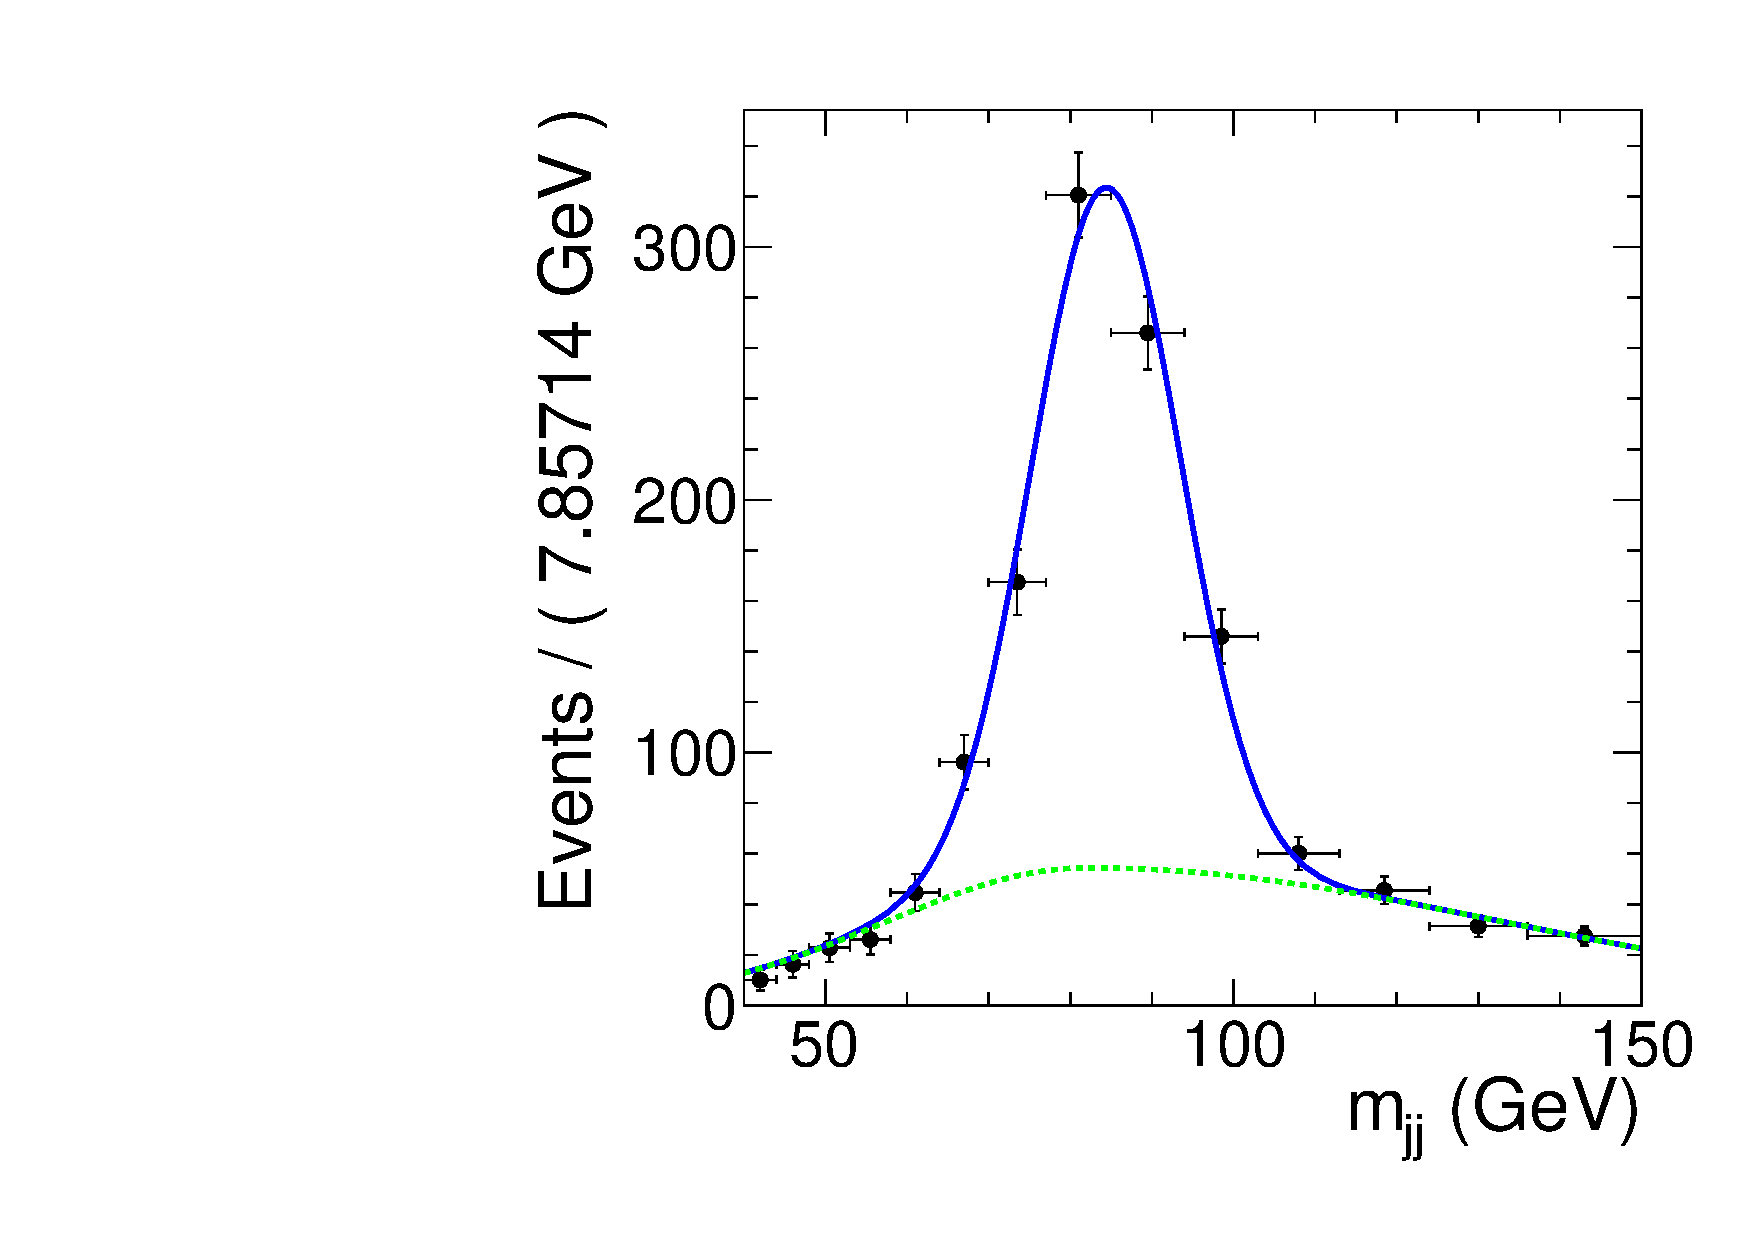
\includegraphics[width=0.45\textwidth]{figs/wpj/WWShape_Diboson_electrons_btagged}
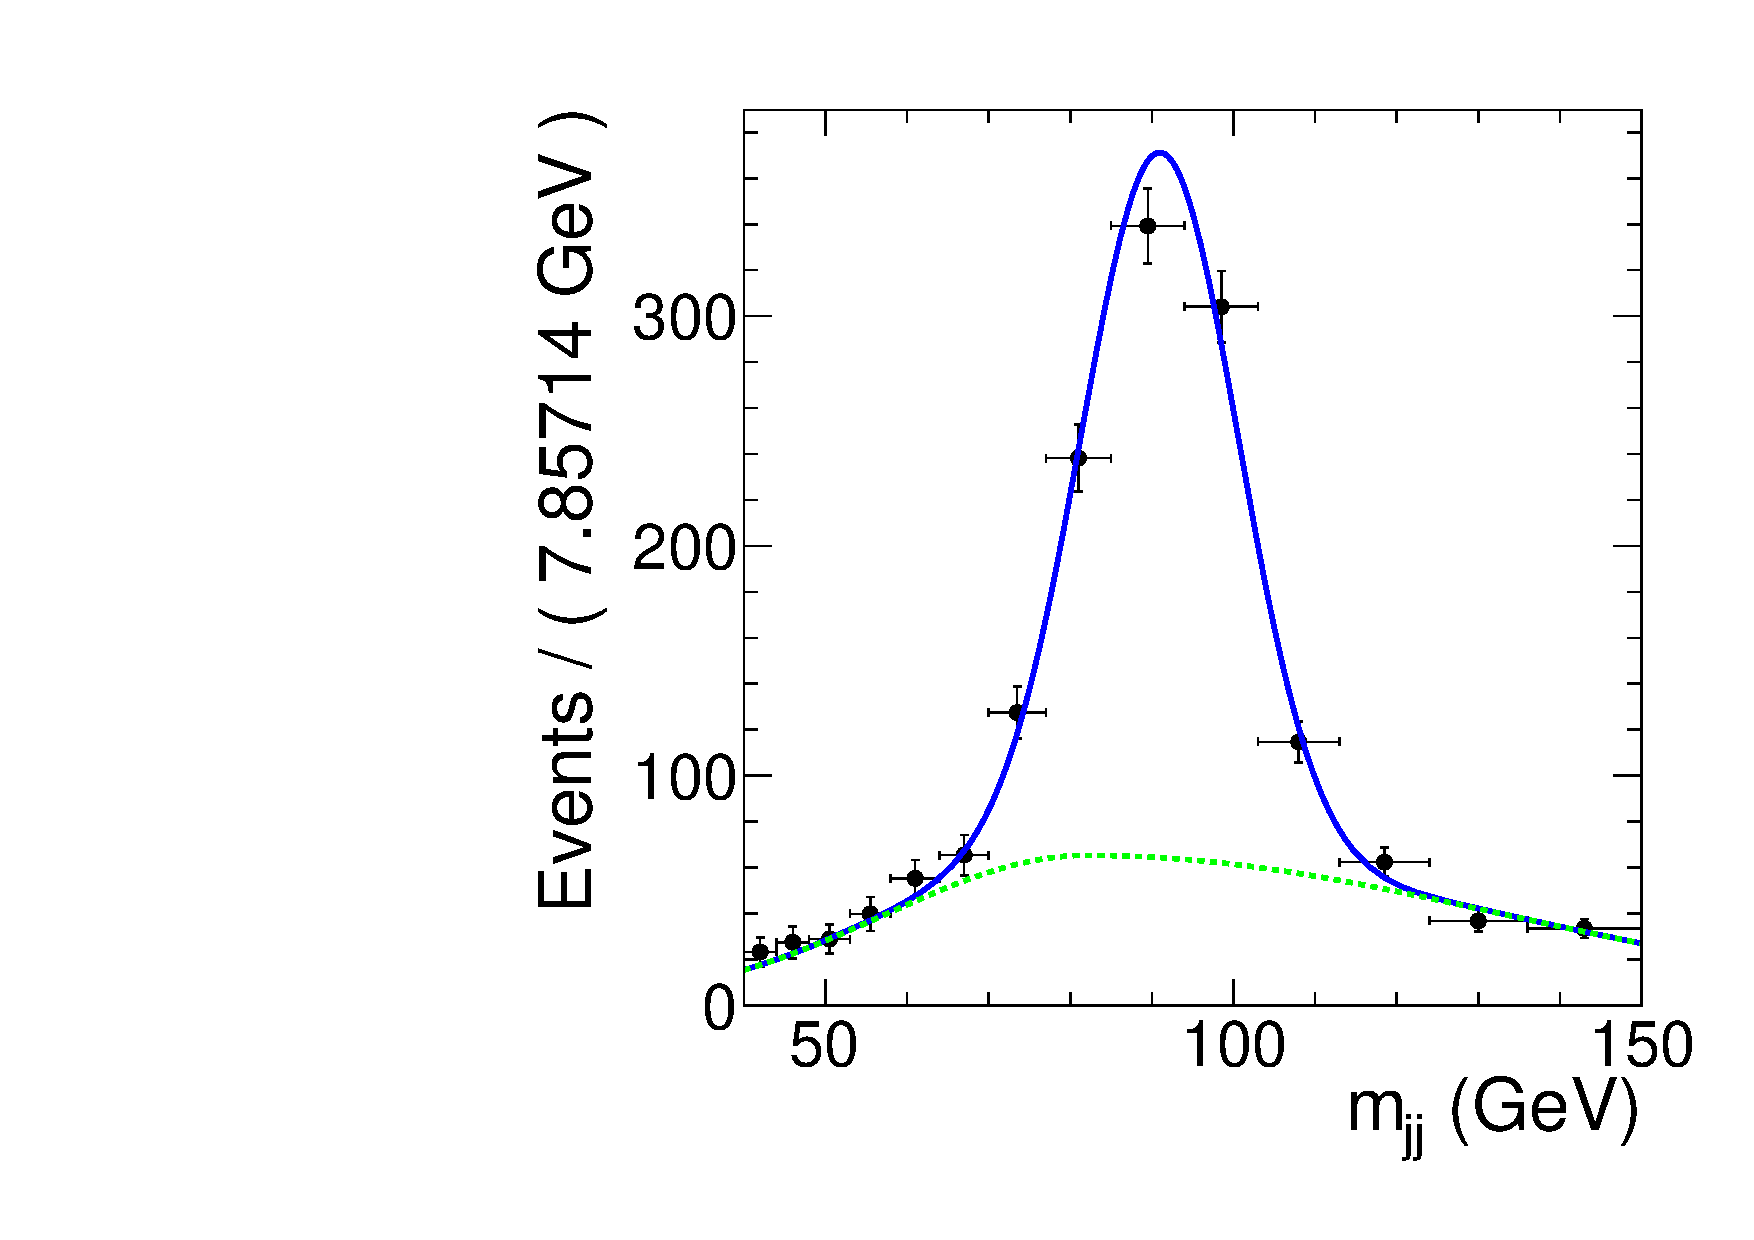
\includegraphics[width=0.45\textwidth]{figs/wpj/WZShape_Diboson_electrons_btagged}
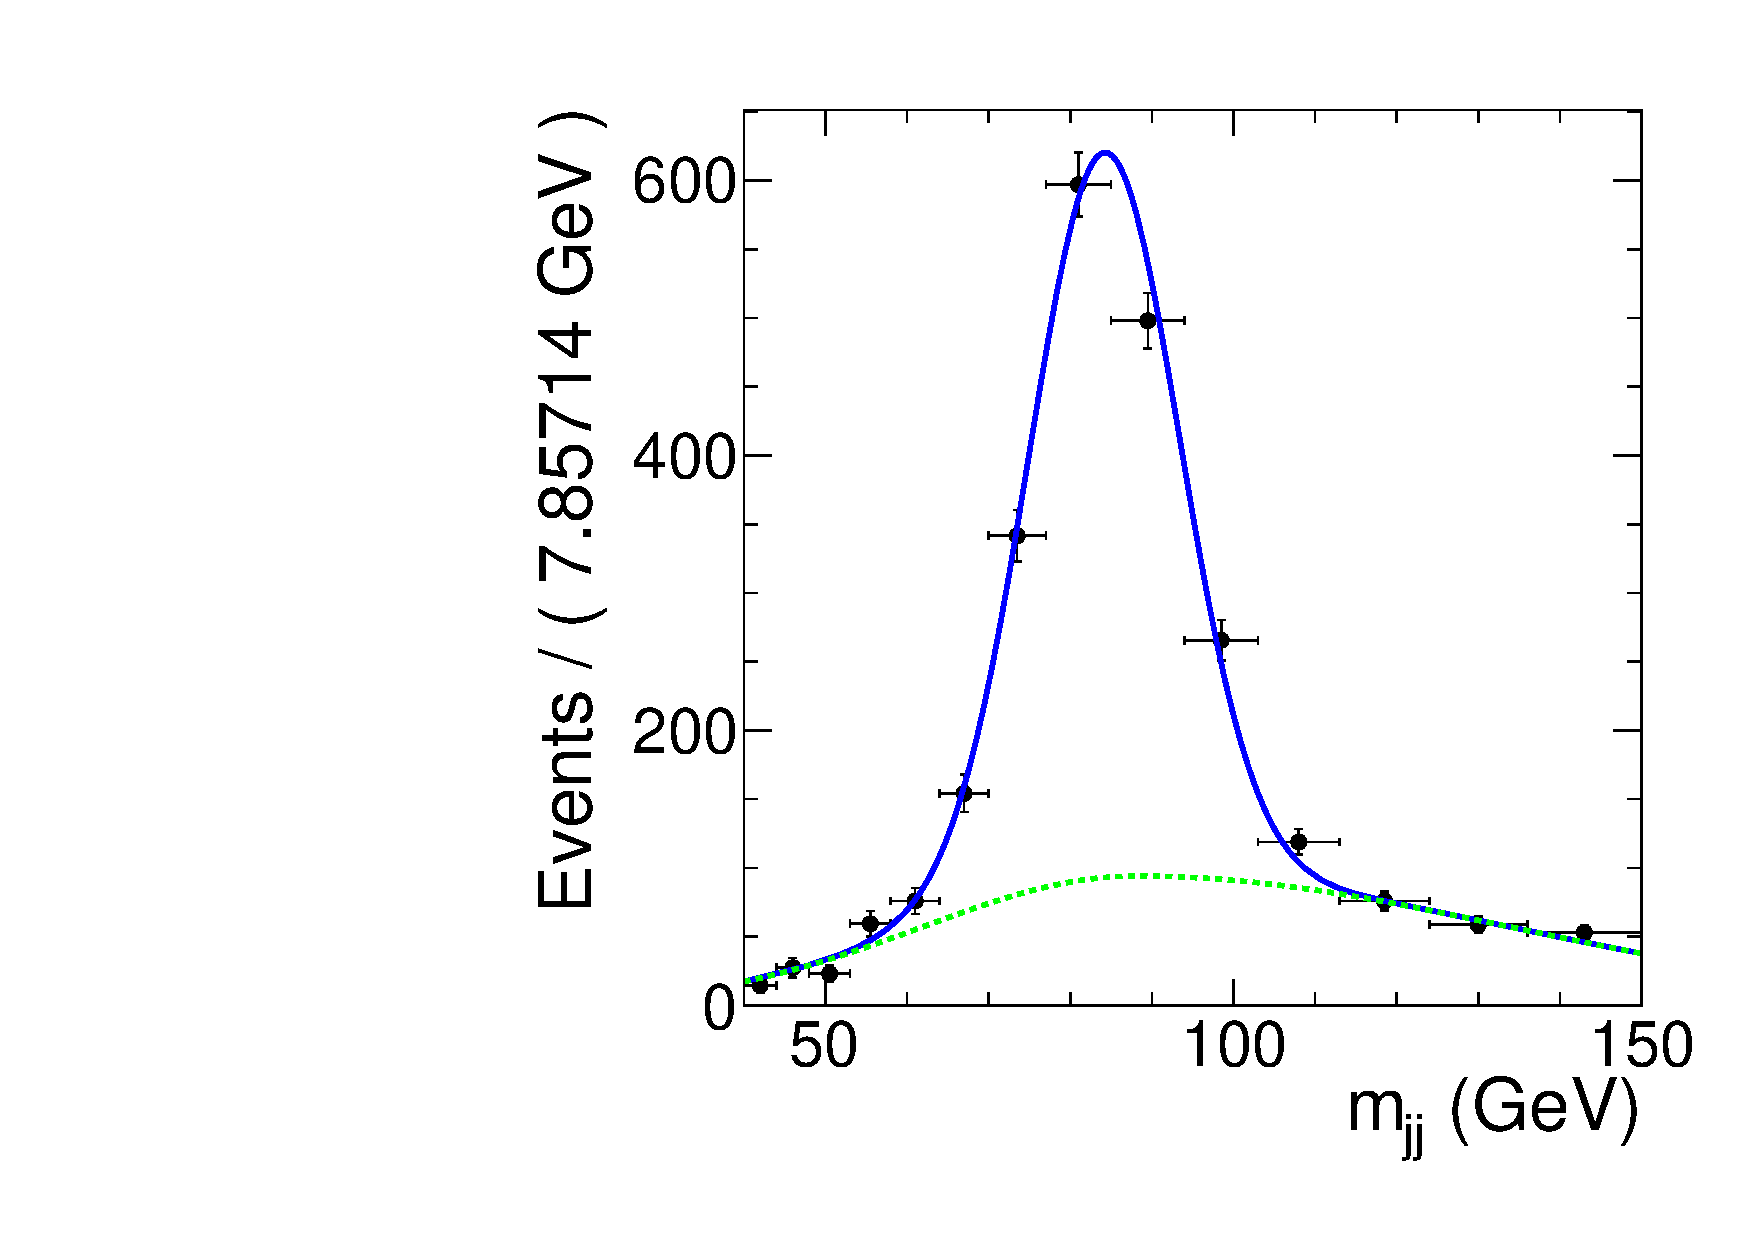
\includegraphics[width=0.45\textwidth]{figs/wpj/WWShape_Diboson_muons_btagged}
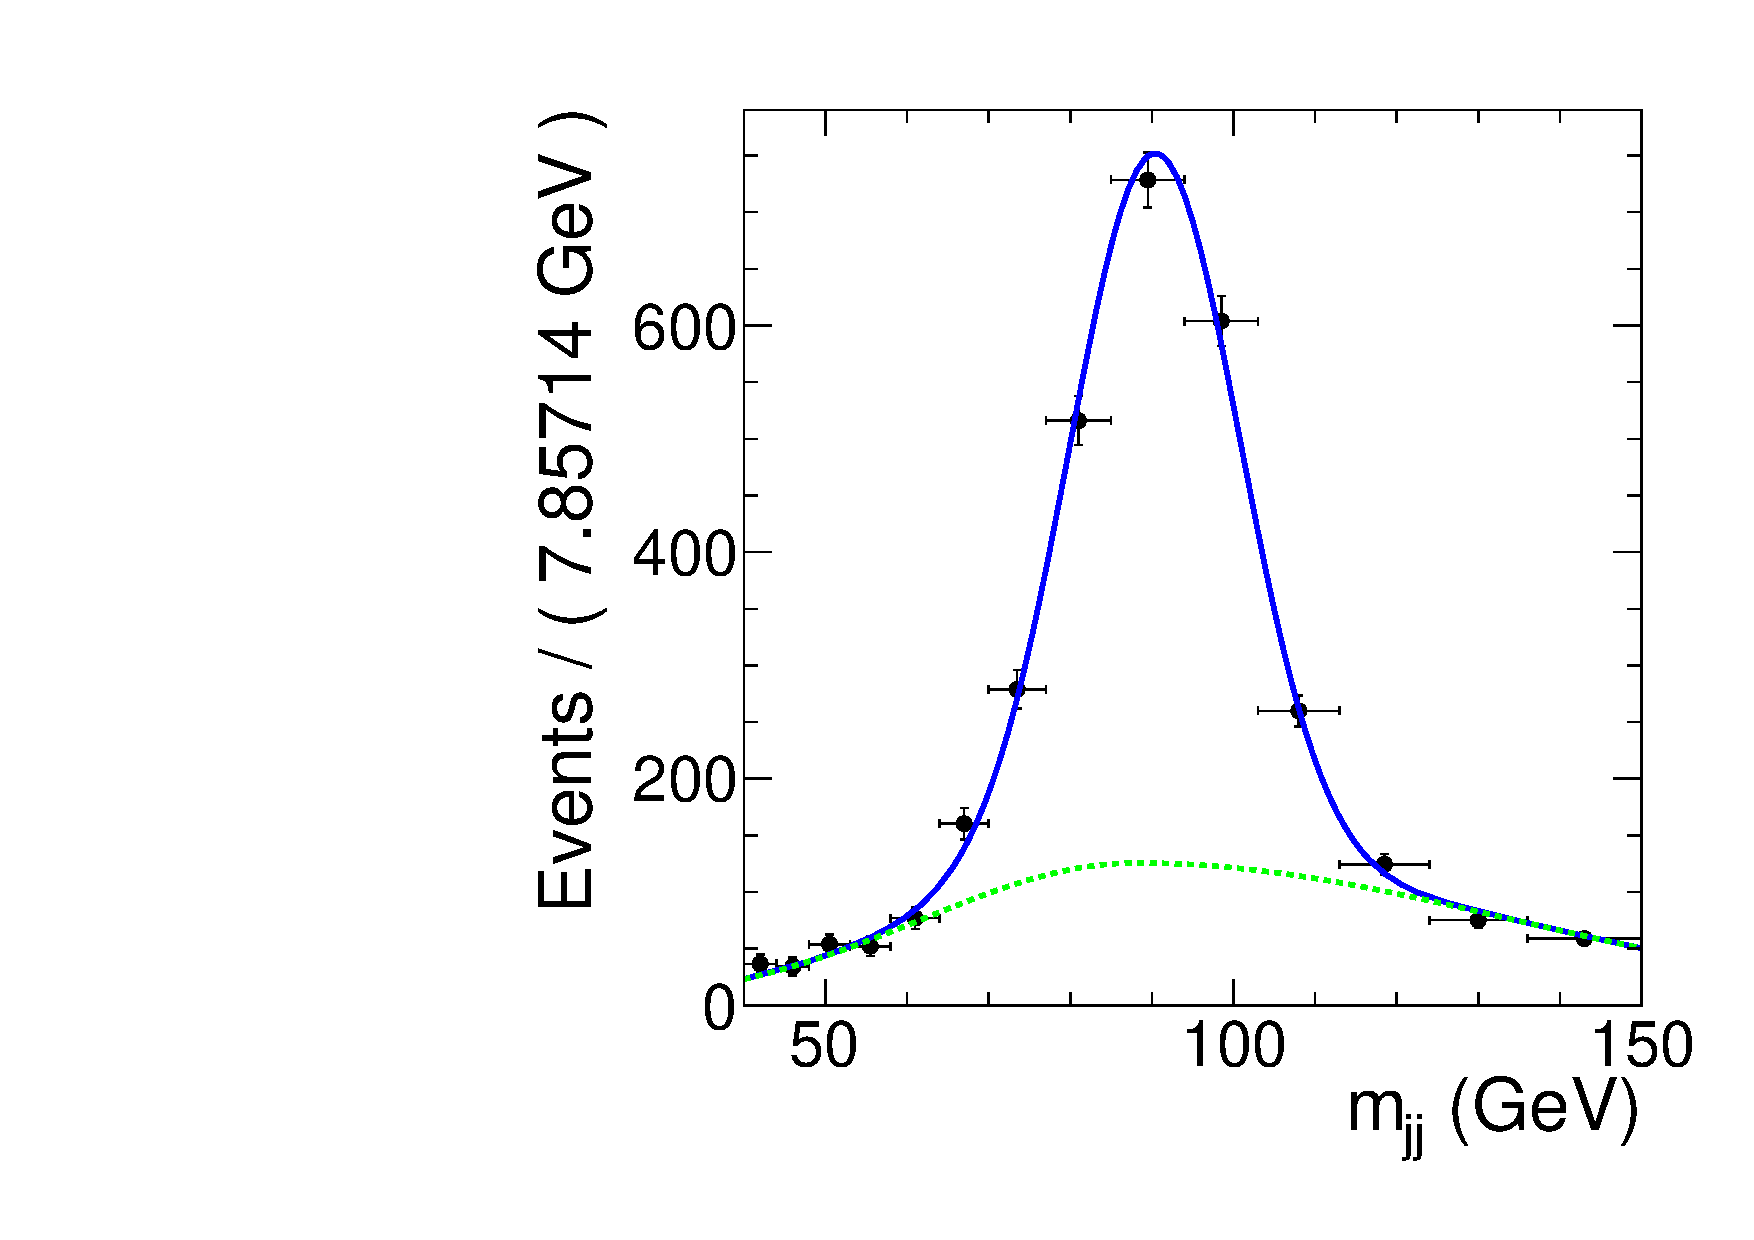
\includegraphics[width=0.45\textwidth]{figs/wpj/WZShape_Diboson_muons_btagged}
\end{center}

\caption{\label{fig:WWWZFit}Diboson shape in the b-tagged sample: Projections of the fit to the diboson MC
samples using the selected parameterization.  Left is WW; right is WZ;
top is electrons; bottom is muons.}

\end{figure}

As was done with the W+jets background shape the parameters of the
shape are Gaussian constrained to those extracted from the MC.
Because the diboson MC does represent a large sample compared to the
integrated luminosity, this represents a tight constraint on the shape
of the signal component.
